\documentclass[12pt,a4paper]{article}
\usepackage{amsmath,amssymb}
\usepackage{graphicx}
\usepackage{booktabs}
\usepackage{hyperref}
\usepackage{natbib}
\usepackage[margin=2.5cm]{geometry}
\usepackage{lineno}
\usepackage{microtype}
\usepackage{caption}
\usepackage{float}
\usepackage{array}
\usepackage{tabularx}

\hypersetup{
    colorlinks=true,
    linkcolor=blue,
    citecolor=blue,
    urlcolor=blue
}

\title{Cascade criticality, therapeutic window emergence,\\
and pre-symptomatic early-warning signals in a\\
connectome-based neurodegeneration framework:\\
an ALS-motivated study on the \textit{C.~elegans} motor circuit}

\author{Maryam Rezaee\\
\small Independent Researcher\\
\small \href{mailto:maryamrezaeenl@gmail.com}{maryamrezaeenl@gmail.com}}

\date{June 2026}

\begin{document}

\maketitle

\begin{quote}
\textbf{CRITICAL DISCLAIMERS:} This is a computational modelling study using the
\textit{C.~elegans} 61-neuron motor connectome as a substrate for studying abstract
degeneration dynamics. It is \textbf{not a clinical model of ALS}, does not use human neural
circuitry, and cannot make predictions about human patients. The \textit{C.~elegans} motor
system differs fundamentally from the human corticospinal-motor neuron system affected in ALS.
All model parameters are chosen for dynamical plausibility, not biological calibration to
measured quantities in any organism. Threshold values, timescales, and parameter ranges are
illustrative. Clinical time-mapping (e.g., ``symptom onset at step 200'') is an analogy for
communication purposes only. \textbf{All results are hypothesis-generating and require
experimental validation before any translational significance can be attributed to them.}
\end{quote}

\begin{abstract}
Amyotrophic lateral sclerosis (ALS) is characterised by progressive motor neuron degeneration
whose mechanisms remain incompletely understood. A key open question is whether degeneration is
a continuous process or involves discrete tipping points, and whether the timing of therapeutic
intervention is intrinsically constrained by circuit-level dynamics. Here we present a
multi-phase computational study using the empirical \textit{C.~elegans} 61-neuron motor
connectome as a tractable substrate for exploring how biophysical feedback loops, network
topology, and aggregation dynamics interact to produce catastrophic collapse.

We implement a nonlinear biophysical cascade (aggregation $\to$ mitochondrial damage $\to$ ATP
collapse $\to$ glutamate excitotoxicity $\to$ calcium overload $\to$ oxidative stress $\to$
aggregation) on the full directed connectome (61 neurons, 127 synapses) and characterise 500
parameter configurations across three dynamical regimes: stable (14.4\%), critical (76.4\%),
and runaway (9.2\%). A three-part falsification criterion reduces the initial 44\% null-model
false-positive rate to 0\%, identifying 247 configurations with genuine triphasic degeneration:
a pre-symptomatic silent phase, rapid collapse, and arrested plateau. Phase~14 stress-testing
reveals a hierarchy of dynamical robustness: spatial coherence and strict tipping-point
structure collapse under severe perturbation ($>$30\% edge dropout, vulnerability $\sigma>0.5$),
while the relative ordering of degeneration aggressiveness remains fully preserved (Spearman
$r=1.000$) even under conditions that destroy all other dynamical structure.

Aggregation suppression therapy consistently outperforms four other therapeutic strategies. The
therapeutic window follows a sharp linear boundary in (strength, start-time) space:
$\mathrm{max\_start\_t} = 425 \times \text{strength} - 237$ for the index configuration,
generalising to mean $252 \times \text{strength} - 107$ across 17 of 20 tested configurations
($R^2 = 0.83$). Robustness testing reveals two disease subtypes differing in aggression and
window shape. An ablation study demonstrates that topological load redistribution constitutes an
independent, aggregation-independent escape mechanism capable of complete collapse in isolation.
All principal findings were robust to four categories of biological noise (synaptic weight
variation, vulnerability score perturbation, connectome edge dropout, and per-neuron aggregation
heterogeneity), with all metrics changing by less than 4\% relative to unperturbed baselines.

Round~2 extended the framework to topology resilience and proof-of-concept early-warning signal
analysis. Sparse-chain topology improved cascade resilience (RES$=0.815$ vs.\ baseline
RES$=0.800$), while triangle-rich feedback loops exhibit a critical safety threshold at
${\sim}60\%$ density beyond which cascade vulnerability increases; no topology modification
widened the therapeutic window, confirming that circuit architecture and drug timing are
independent intervention axes. Three pre-symptomatic biomarkers measured at $t=50$ (before any
neuron death) achieved 87\% simulated subtype classification accuracy (Phase~R2.8 TWE pipeline) and
achieved 86.8\% of the oracle-defined benefit within this simulation framework,
with within-subtype parameter heterogeneity --- not stochastic noise ---
identified as the dominant irreducible error source.

These results generate testable hypotheses about the necessity of pre-symptomatic intervention,
the primacy of protein aggregation seeding as a disease driver, and the proof-of-concept
potential of simulated model-derived early-warning proxies for hypothesis-generating therapeutic triage, while
underscoring that all findings
remain model-specific and require experimental corroboration.

\smallskip
\noindent\textit{Keywords:} neurodegeneration model; connectome; tipping points; therapeutic
window; protein aggregation; ALS; \textit{C.~elegans}; model-derived early-warning proxies;
topology resilience; cascade criticality
\end{abstract}

\tableofcontents
\newpage

%% ============================================================
\section{Introduction}
%% ============================================================

\subsection{Background and motivation}

A central challenge in computational neurodegeneration modelling is distinguishing genuine
dynamical phenomena --- tipping points, therapeutic windows, disease subtypes --- from model
artifacts. Here, using ALS as a motivating biological context and the \textit{C.~elegans} motor
connectome as a principled network substrate, we develop and stress-test a multi-phase framework
for studying cascade criticality and intervention timing in biophysically-coupled network
degeneration models.

Amyotrophic lateral sclerosis is a fatal neurodegenerative disease characterised by progressive
loss of both upper and lower motor neurons, leading to paralysis and death, typically within two
to five years of symptom onset \citep{vanes2017}. Despite advances in understanding molecular
mechanisms --- including TDP-43 pathology \citep{neumann2006}, C9ORF72 repeat expansions
\citep{dejesus2011}, and SOD1 misfolding \citep{rosen1993} --- the disease remains almost
universally fatal, with only modest survival benefits from current therapeutics (riluzole,
edaravone, sodium phenylbutyrate/taurursodiol).

A recurring clinical observation is that significant neurodegeneration may precede symptom
onset by months to years \citep{turner2012,benatar2019}. The ATLAS trial of tofersen, an
antisense oligonucleotide targeting SOD1, demonstrated that pre-symptomatic intervention in
biomarker-positive carriers could delay phenoconversion \citep{benatar2023}. This raises a
fundamental theoretical question: is there an inherent, mechanistically-determined therapeutic
window, and if so, what determines its width?

Separately, it is increasingly appreciated that ALS is heterogeneous \citep{alchalabi2017}:
patients vary markedly in onset site, progression rate, extramotor involvement, and survival.
Whether this heterogeneity reflects distinct disease subtypes with qualitatively different
dynamics, or a continuum of the same underlying process, has implications for patient
stratification and clinical trial design.

\subsection{The \textit{C.~elegans} connectome as a model substrate}

\textit{Caenorhabditis elegans} has a fully mapped nervous system
\citep{white1986,cook2019} comprising 302 neurons with complete synaptic connectivity. Its
motor circuit --- approximately 61 neurons with 127 directed synapses --- is compact enough for
exhaustive computational analysis while retaining genuine biological wiring rather than a
synthetic graph approximation. The motor neurons include dorsal and ventral A-, B-, and D-type
motor neurons (DA, DB, DD, VA, VD) with well-characterised vulnerability profiles to cellular
stress.

We use this connectome not as a model of \textit{C.~elegans} neurobiology per se, but as a
principled network substrate on which to impose ALS-relevant biophysical dynamics. This
approach allows us to separate the contributions of network topology from biochemical feedback
strength, in a system where topology is empirically determined rather than assumed.

\textbf{We emphasise that this is not a model of ALS in nematodes or humans.}
\textit{C.~elegans} does not develop ALS. Its motor system differs from the human
corticospinal-motor neuron system in every relevant respect: scale, architecture, cell type,
and disease susceptibility. All results should be interpreted as dynamical properties of an
abstract model on a biologically-derived graph.

\subsection{Gaps addressed and contributions}

This study addresses three gaps in computational ALS/neurodegeneration modelling:

\begin{enumerate}
\item \textbf{Tipping point falsification}: Existing network neurodegeneration models rarely
subject claimed tipping points to rigorous null-model control. We develop and apply a
three-part falsification criterion that reduces a 44\% null-model false-positive rate to 0\%.

\item \textbf{Topology vs.\ dynamics}: Whether degeneration patterns in connectome models are
primarily driven by the specific wiring or by the underlying biochemical dynamics is rarely
directly tested. We do so across five network types (Phases~5--14) and nine structural variants
(Round~2).

\item \textbf{Therapeutic window quantification and proof-of-concept early-warning signal analysis}: We map the exact
(strength, timing) boundary separating prevention from failure, characterise two disease
subtypes, and --- in Round~2 --- demonstrate that pre-symptomatic biomarkers at the $t=50$
equivalent can assign intervention strategy with 87\% subtype accuracy and 86.8\% oracle
efficiency.
\end{enumerate}

%% ============================================================
\section{Methods}
%% ============================================================

\subsection{Connectome data}

The motor connectome was derived from the \textit{C.~elegans} physical wiring diagram
\citep{white1986,cook2019}. We use 61 neurons with 127 directed chemical synapses in the motor
circuit. Synaptic weights are derived from synapse counts. Vulnerability scores ---
representing each neuron's intrinsic susceptibility to aggregation-driven damage --- are
assigned based on neuron type: motor neurons (DA, DB, DD, VA, VD) receive scores of 0.65--1.00
reflecting their established sensitivity to cellular stress.

\textbf{Parameter range justification.} Parameter ranges were selected to span subcritical,
critical, and supercritical dynamical regimes rather than to match biological measurements.
\texttt{aggregationAmplification} spans $[0.05, 20.0]$ (log-uniform) to cover the full range
from near-zero cascade to runaway collapse; the other six parameters were set to ranges wide
enough that the critical regime occupies a substantial fraction of parameter space (76.4\% of
500 sampled configurations), ensuring sufficient data for subtype and boundary analysis. These
ranges are not intended as estimates of biological quantities in any organism.

The connectome does not include the
DVA interneuron, which appears in simplified circuit diagrams but is absent from the canonical
motor circuit reconstruction; the AVDL interneuron (index~12) serves as a structural proxy for
high-connectivity interneuron function in relevant analyses. All simulation phases are
interactively visualisable at \url{https://als-connectome-dashboard.vercel.app}.

\subsection{Biological state variables}

Each neuron $i$ carries four continuous state variables updated at each timestep $\Delta t = 1$:

\begin{itemize}
\item \textbf{Health} $h_i \in [0, 1]$: fractional functional integrity; neuron is dead when
$h_i < 0.15$.
\item \textbf{Aggregation load} $a_i \in [0, \infty)$: normalised misfolded protein burden,
analogous to TDP-43 or SOD1 aggregate density.
\item \textbf{ATP} $e_i \in [0, 1]$: relative bioenergetic status; irreversible collapse locks
at $e_i = 0$ once both $e_i < \theta_{\text{ATP}}$ and $a_i > \theta_{\text{irrev}}$
simultaneously.
\item \textbf{Glutamate drive} $g_i$: synaptic glutamate accumulation arising from reuptake
failure under ATP depletion.
\end{itemize}

These variables are updated each step through coupled differential equations encoding the
excitotoxic cascade described below.

\clearpage
\subsection{Excitotoxic feedback cascade}

The model implements six coupled feedback mechanisms forming a closed positive-feedback loop:

\begin{quote}
\begin{tabbing}
\hspace{2cm}\=\hspace{5.5cm}\=\kill
\>\texttt{aggregation}\\
\>$\rightarrow$ \texttt{mitochondrial damage} \>(\texttt{mitochondrialFragility})\\
\>$\rightarrow$ \texttt{ATP collapse} \>(\texttt{atpCollapseThreshold})\\
\>$\rightarrow$ \texttt{glutamate accumulation} \>(\texttt{glutamateSensitivity} $\times$
reuptake failure)\\
\>$\rightarrow$ Ca$^{2+}$ overload \>(\texttt{calciumStressGain} $\times$ NMDA activation)\\
\>$\rightarrow$ \texttt{oxidative stress} \>(ROS from Ca$^{2+}$)\\
\>$\rightarrow$ \texttt{aggregation seeding} \>(\texttt{oxidativeFeedback}) $\leftarrow$
closes the loop\\
\end{tabbing}
\end{quote}

The four state variables evolve according to:

\begin{align}
\frac{da_i}{dt} &= \alpha \cdot \texttt{aggAmp} \cdot a_i(1-a_i)
  + \beta \sum_{j \in \mathcal{N}(i)} a_j \cdot w_{ji} + \gamma \cdot \text{ROS}_i
  \label{eq:agg}\\
\frac{de_i}{dt} &= \rho_e(1-e_i) - \kappa \cdot a_i - \delta \cdot \text{load}_i
  \label{eq:atp}\\
\frac{dg_i}{dt} &= \sigma \cdot (1-e_i) - \lambda \cdot \text{astro}_i \cdot g_i
  \label{eq:glut}\\
\frac{dh_i}{dt} &= -\eta \cdot \text{stress}_i + \mu \cdot e_i \cdot (1-a_i)
  \label{eq:health}
\end{align}

where $\text{stress}_i = w_1 \cdot \text{overload}_i + w_2 \cdot a_i + w_3 \cdot g_i$,
$\mathcal{N}(i)$ is the set of neurons projecting to neuron $i$, and $w_{ji}$ is the synaptic
weight from $j$ to $i$. Parameters $\alpha, \beta, \gamma, \rho_e, \kappa, \delta, \sigma,
\lambda, \eta, \mu$ correspond to the named simulation parameters; full values in Supplementary
Table~S1.

\textbf{Irreversibility switch}: when a neuron simultaneously satisfies $e_i <
\theta_{\text{ATP}}$ and $a_i > \theta_{\text{irrev}}$, its \texttt{irreversible} flag is set.
From this point, health can only decrease; the neuron is committed to degeneration. This models
the clinical observation that neurons past a bioenergetic threshold cannot recover energy
homeostasis.

\textbf{Aggregation seeding and spread}: The aggregation term drives both intrinsic growth
(within a neuron) and prion-like spread (to synaptic neighbours). The scaling factor
\texttt{aggregationAmplification} acts as a bifurcation parameter: below a critical value, the
loop gain is insufficient to sustain spreading; above it, the cascade becomes self-amplifying.
Log-uniform sampling is applied to this parameter and to \texttt{glutamateSensitivity} and
\texttt{oxidativeFeedback}, as these span multiple orders of magnitude in biological systems.

Seven free parameters are explored (Table~\ref{tab:params}). \textit{(Parameter names use
camelCase as implemented in the simulation code.)}

\begin{table}[H]
\centering
\caption{Model parameters, ranges, and biological analogues.}
\label{tab:params}
\begin{tabularx}{\textwidth}{lllX}
\toprule
\textbf{Parameter} & \textbf{Range} & \textbf{Sampling} & \textbf{Biological analogue}\\
\midrule
\texttt{aggregationAmplification} & $[0.05,\,20.0]$ & log-uniform &
  TDP-43/FUS prion-like seeding efficiency\\
\texttt{mitochondrialFragility} & $[0.3,\,8.0]$ & uniform &
  PINK1/Parkin pathway, Complex~I deficit\\
\texttt{atpCollapseThreshold} & $[0.05,\,0.7]$ & uniform &
  Bioenergetic point of no return\\
\texttt{glutamateSensitivity} & $[0.0005,\,0.1]$ & log-uniform &
  EAAT2 glutamate transporter expression\\
\texttt{calciumStressGain} & $[0.02,\,5.0]$ & uniform &
  NMDA receptor density\\
\texttt{oxidativeFeedback} & $[0.0005,\,0.5]$ & log-uniform &
  SOD1 activity / antioxidant reserve\\
\texttt{recoveryIrreversibility} & $[0.2,\,0.99]$ & uniform &
  Autophagic clearance capacity\\
\bottomrule
\end{tabularx}
\end{table}

\subsection{Regime classification}

500 parameter configurations were run for 500 timesteps each. Three regimes are defined:

\begin{itemize}
\item \textbf{Stable}: $>$50 neurons alive at $t = 500$ (network resists degeneration).
\item \textbf{Critical}: $\geq 10$ alive at $t = 200$ AND $\leq 50$ alive at $t = 500$
(sustained, partial collapse).
\item \textbf{Runaway}: $<$10 alive by $t = 200$ (rapid near-complete collapse).
\end{itemize}

The critical regime is the focus of subsequent analysis; it corresponds to sustained
intermediate degeneration most consistent with clinical ALS progression.

All results are reported in simulation steps only. Day equivalents in the Discussion are
order-of-magnitude analogies based on a single-anchor calibration (step~200 $\approx$ ALS
symptom onset $\approx$ 15~months) and must not be interpreted as calibrated predictions.

\subsection{Tipping point criterion --- falsification approach}

An initial single-threshold criterion (alive $< 55$ at any step) produced a 44\% false-positive
rate against an independent null model in which neurons decline via uncoupled random walks with
no synaptic coupling or biochemical feedback. This prompted development of a three-part strict
criterion:

\begin{itemize}
\item \textbf{C1 --- Slope}: peak 10-step neuron death rate $> 4$ (sudden acceleration).
\item \textbf{C2 --- Spatial coherence}: Pearson $r$ between each neuron's vulnerability score
and its death step $> 0.30$ (death order correlated with vulnerability, as expected from
synaptic spread).
\item \textbf{C3 --- Silent phase}: first neuron death after step~50 (clinically meaningful
pre-symptomatic window).
\end{itemize}

All three conditions must be satisfied simultaneously. Under this criterion, the null model
false-positive rate falls from 44\% to 0\% (0/100 runs), while 247/382 critical configurations
(64.7\%) are classified as exhibiting genuine tipping points.

\subsection{Therapy model}

Therapeutic interventions are modelled as time-limited or continuous modifications to model
parameters, initiated at a prescribed start time $t_{\text{start}}$:

\begin{itemize}
\item \textbf{Aggregation suppression} (\texttt{agg\_sup}): multiplies
\texttt{aggregationAmplification} by $(1 - \text{strength})$. Analogues: tofersen (SOD1
antisense oligonucleotide), BIIB078 (C9ORF72 ASO).
\item \textbf{Metabolic support} (\texttt{met\_sup}): boosts ATP recovery rate.
\item \textbf{Glutamate suppression} (\texttt{glut\_sup}): reduces
\texttt{glutamateSensitivity}. Analogue: riluzole.
\item \textbf{Astrocyte support} (\texttt{astro\_sup}): increases toxin clearance.
\item \textbf{Adaptive} (\texttt{adaptive}): biomarker-triggered combination therapy
(activates when mean aggregation exceeds a threshold).
\end{itemize}

Therapies are scored on four metrics: tipping delay, functional duration gain, plateau survivor
gain, and key-neuron survival rate.

\subsection{Load redistribution model}

A separate simulator (Phase~7D, Escape~3; Phase~8) tests pure topological cascade dynamics with
all biochemistry disabled. Neuron health declines from an intrinsic vulnerability term and a
load term proportional to the fraction of dead upstream partners:

\begin{equation}
\frac{dh_i}{dt} = -\!\left(\lambda_{\text{int}} \cdot v_i
  + \lambda_{\text{load}} \cdot f_i^{\text{dead}}\right)
\label{eq:load}
\end{equation}

where $v_i$ is vulnerability and $f_i^{\text{dead}}$ is the fraction of neurons projecting to
$i$ that are already dead. Parameters $\lambda_{\text{int}} = 0.004$ and $\lambda_{\text{load}}
= 0.006$ are chosen so that load redistribution is insufficient alone at low death counts but
becomes self-sustaining once several neurons have died.

\subsection{Cluster analysis}

Unsupervised subtype analysis uses K-means clustering ($K = 2, 3, 4, 5$) with 50 random
initialisations and silhouette score selection. PCA (numpy eigenvector decomposition) provides
dimensionality reduction for visualisation. Bootstrap stability is assessed over 100
resamplings at 80\% of configurations; per-pair stability scores are computed as the fraction
of bootstrap runs in which a given pair of configurations is assigned the same cluster. All
implementations use pure numpy/stdlib to avoid dependency on external ML libraries whose
results may vary across versions.

\subsection{Biological noise robustness testing}

To assess whether the identified tipping point structure and disease subtypes are robust to
parameter uncertainty, we applied four categories of biological noise independently to the
top-10 genuine critical configurations (Phase~7B) using 20 random seeds per perturbation level
and 500 simulation steps per run:

\begin{enumerate}
\item \textbf{Synaptic weight noise} ($\sigma = 5\%, 10\%, 20\%$): Multiplicative Gaussian
noise applied to all non-zero entries of \texttt{agg\_W} and \texttt{excitotox\_W}; negative
values clipped to zero.
\item \textbf{Vulnerability score noise} ($\sigma = 0.05, 0.10, 0.20$): Additive Gaussian
noise applied to each neuron's vulnerability score, clipped to $[0, 1]$.
\item \textbf{Connectome edge dropout} (2\%, 5\%, 10\%): A random fraction of directed
synapses removed simultaneously from \texttt{agg\_W} and \texttt{excitotox\_W}.
\item \textbf{Heterogeneous per-neuron aggregation amplitude} ($\pm 20\%$): Each neuron
received a distinct \texttt{aggAmp} value drawn uniformly from $[0.8 \times \text{base},\,
1.2 \times \text{base}]$; both the neuron's vulnerability score and the corresponding row of
\texttt{agg\_W} were scaled by the per-neuron factor, preserving the proportional relationship
between intrinsic seeding and synaptic spread.
\end{enumerate}

Robustness was quantified for three metrics: mean tipping step (relative drift from baseline),
spatial coherence $r$ (relative change from baseline), and genuine tipping rate (absolute
change). Verdicts: relative change $< 10\%$ = robust; $10$--$30\%$ = moderately sensitive;
$> 30\%$ = fragile. For perturbation~4, subtype separation was additionally assessed via
Spearman rank correlation between baseline and perturbed tipping steps across the ten
configurations.

\subsection{Breaking threshold probe}

To identify the upper limits of model robustness and characterise a hierarchy among dynamical
properties, we applied two severe perturbation types to the top-5 genuine critical
configurations using 10 seeds per level and 300 simulation steps:

\begin{enumerate}
\item \textbf{Extreme edge dropout} (30\%, 50\%, 70\% of directed synapses removed): After
dropout, the undirected adjacency graph was tested for connectivity via depth-first search; if
disconnected, all edges outside the largest connected component were zeroed, restricting
dynamics to that component.
\item \textbf{Extreme vulnerability noise} ($\sigma = 0.50$, $\sigma = 1.00$): Additive
Gaussian noise applied to vulnerability scores, clipped to $[0.01, 1.0]$.
\end{enumerate}

For each condition, four metrics were recorded: genuine tipping rate, mean spatial coherence
$r$, mean tipping step, and subtype rank preservation (Spearman $r$ between baseline and
perturbed tipping steps across the five configurations). Breaking points were identified as the
first perturbation level at which each metric crossed its threshold: genuine rate $< 0.5$,
coherence $r < 0.3$, subtype rank $r < 0.5$.

\subsection{Round~2: Topology resilience and pre-symptomatic biomarker analysis}

Round~2 comprises eight additional analysis phases (R2.1--R2.8), using all 247 genuine
critical configurations from Phase~12 unless otherwise noted:

\begin{itemize}
\item \textbf{Phases R2.1--R2.2 (Motif resilience and efficiency tradeoff)}: Nine structural
variants of the connectome (sparse chain, distributed, anti-hub, modular, bypass loops,
hierarchical, rich club, triangle rich, baseline) compared via composite RES score
$= (\text{tipping delay ratio} \times \text{therapy window ratio} \times \text{plateau ratio})
- \text{variance penalty}$, computed over 5 configurations $\times$ 10 seeds $\times$ 500 steps.
Efficiency-resilience landscape mapped across 6 topology families $\times$ 7 strength levels.

\item \textbf{Phase R2.3 (Topology-therapy boundary)}: Therapeutic boundary re-measured on 4
topology variants using a $9 \times 9$ strength $\times$ start\_t grid with 5 seeds per point.

\item \textbf{Phase R2.4 (Subtype $\times$ topology)}: Five representative configs per cluster
$\times$ 4 topologies $\times$ 5 seeds $\times$ 300 steps.

\item \textbf{Phases R2.5--R2.7 (Simulated early-warning panel)}: Early dynamics at $t=50$ and $t=100$
(seed~42, 150 steps) extracted for all 247 configs; 10-fold cross-validated logistic and ridge
regression predicting subtype, tipping step, therapy window width, and therapy success
probability.

\item \textbf{Phase R2.8 (Therapeutic Window Estimator)}: 10-fold CV out-of-fold predictions
on all 247 configs; 3-seed virtual triage simulation totalling 3,705 runs; oracle strategies
derived from full $(3 \times 4 \times 5)$-grid therapy sweeps.
\end{itemize}

This study is presented with 16 figures (fig01--fig16). Figures~1--9 cover Phases~5--14;
Figures~10--16 cover Round~2 analyses.

%% ============================================================
\clearpage
\section{Results}
%% ============================================================

\subsection{Phase~5: Criticality emergence and regime structure}

Parameter screening of 500 configurations revealed three distinct dynamical regimes. The
majority of configurations (382/500, 76.4\%) fell in the critical regime, defined by sustained
partial degeneration across the full 500-step simulation. Stable configurations (72/500, 14.4\%)
maintained most neurons alive, while runaway configurations (46/500, 9.2\%) collapsed almost
completely before step~200 (Figure~\ref{fig:regimes}).

\begin{figure}[H]
\centering
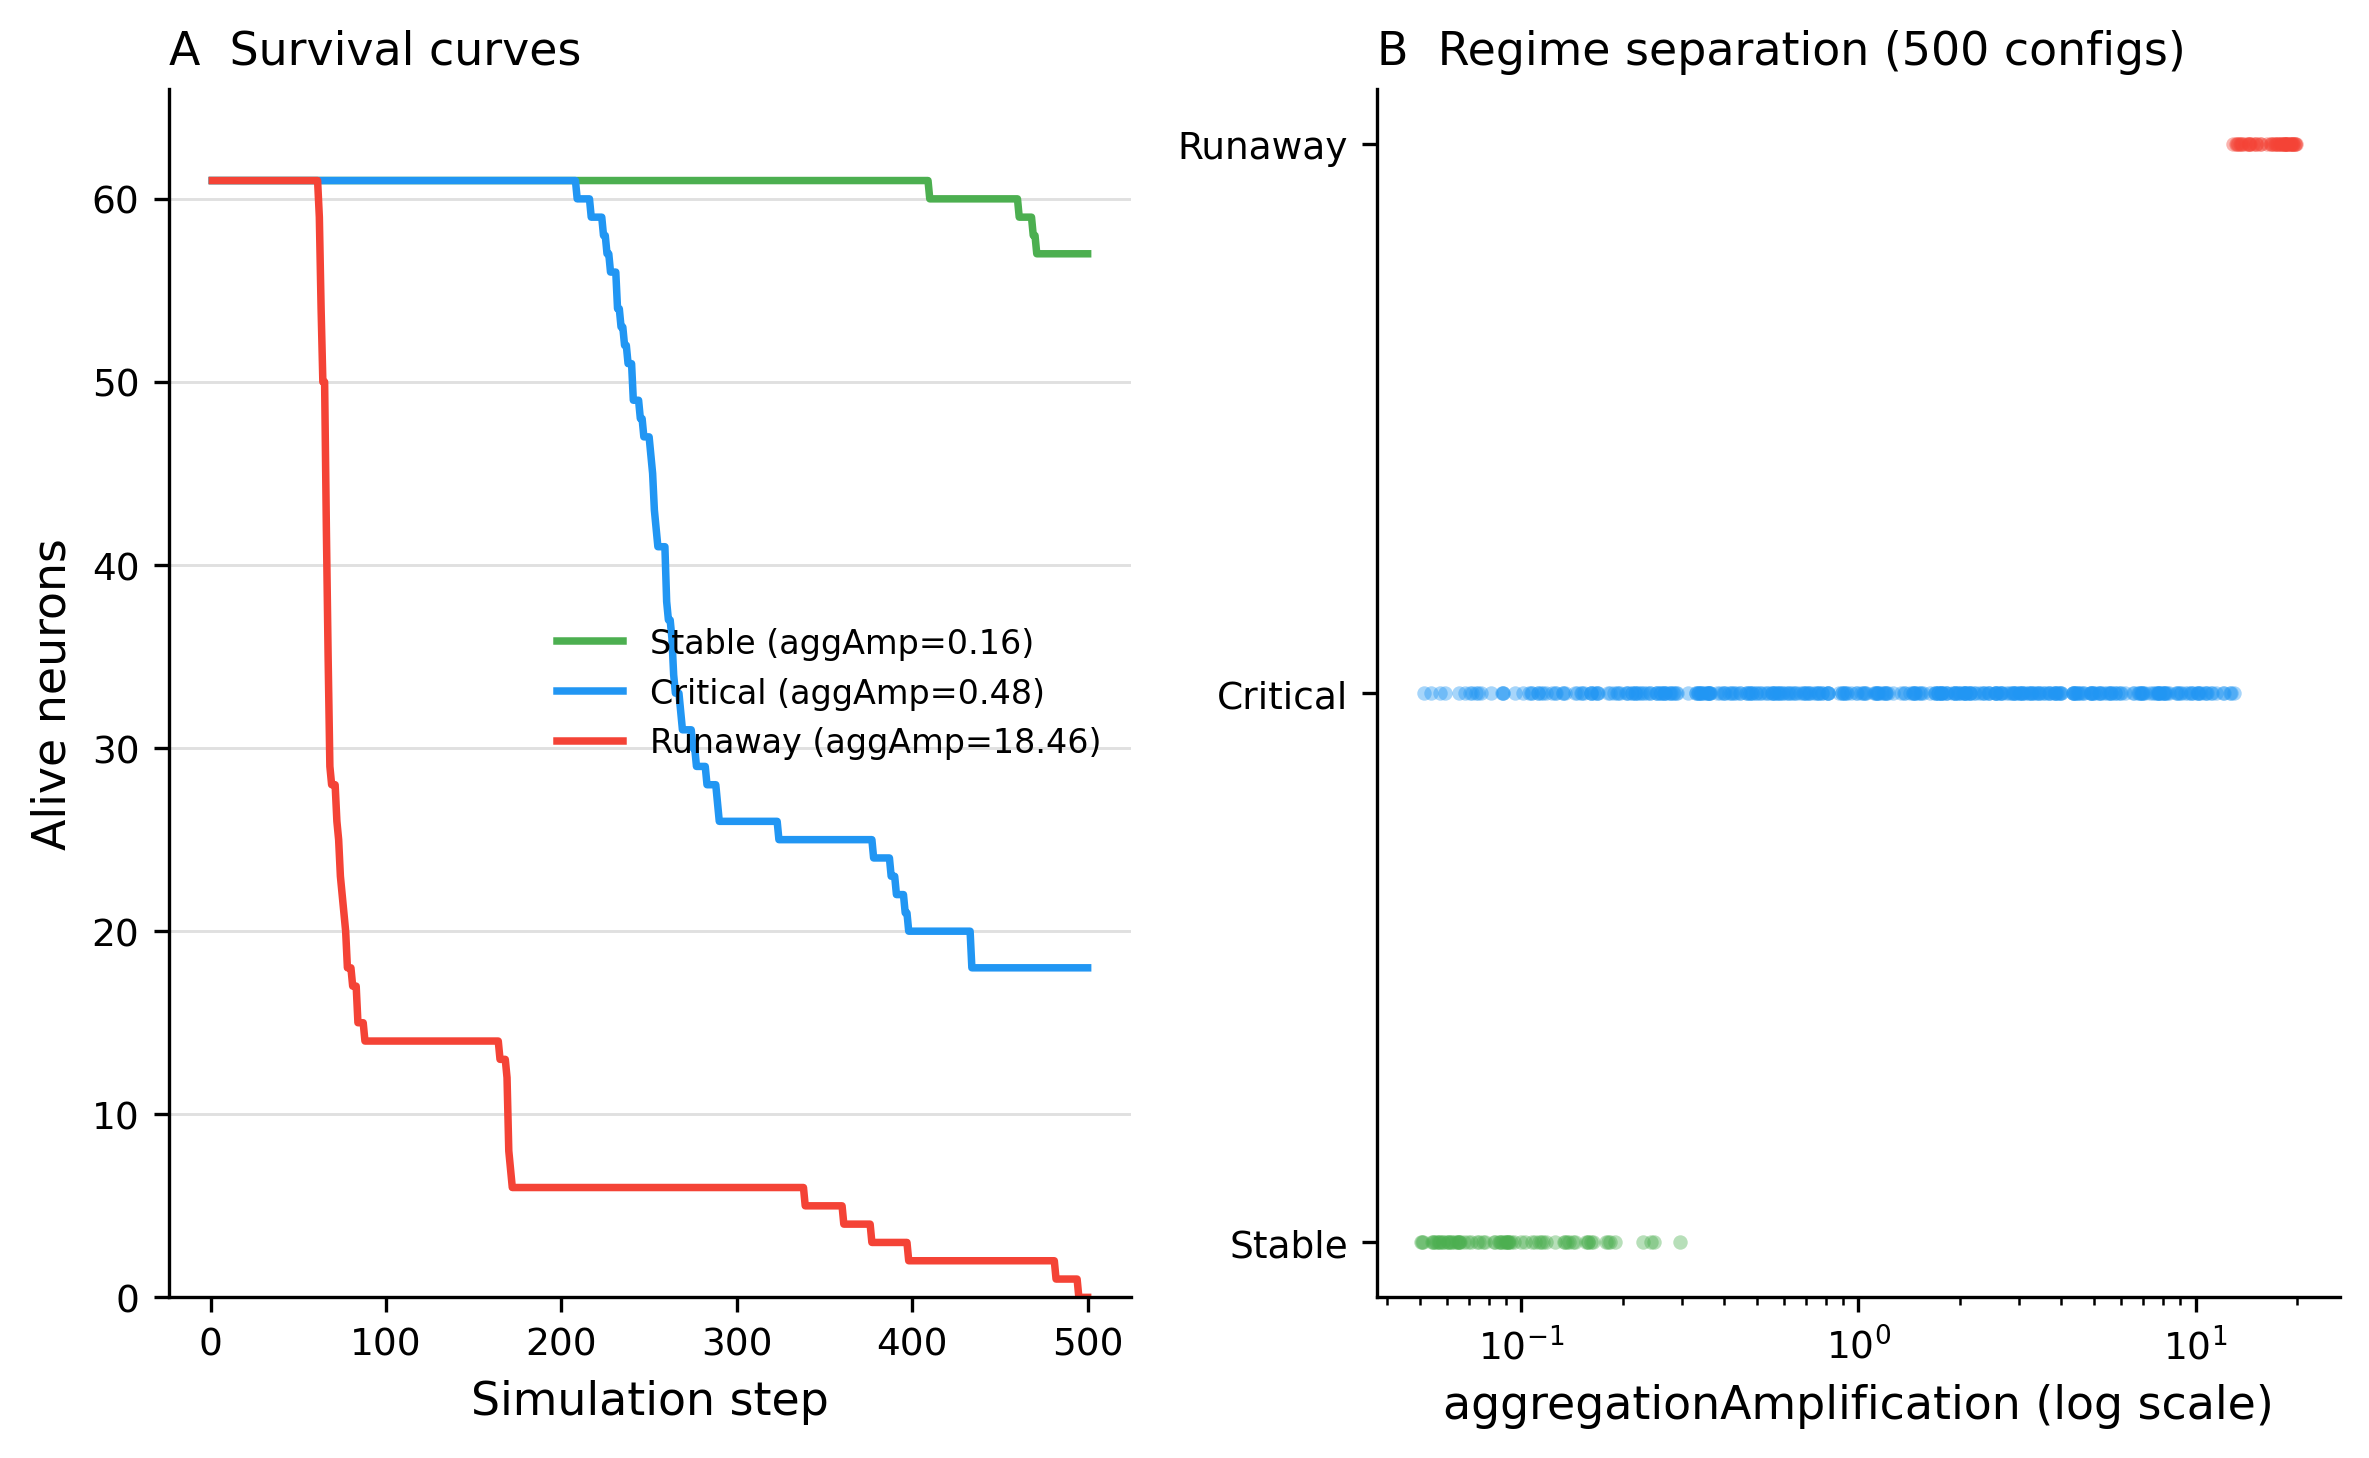
\includegraphics[width=0.9\textwidth]{figures/fig1_supplementary_regimes.png}
\caption{Regime structure and survival curves. 500 configurations classified into stable
(14.4\%), critical (76.4\%), and runaway (9.2\%) regimes. Supplementary panel shows
representative survival curves for each regime.}
\label{fig:regimes}
\end{figure}

\textbf{Aggregation amplitude as the dominant bifurcation parameter.} Regime-separation
analysis ranked all seven parameters by discriminating power. \texttt{aggregationAmplification}
was overwhelmingly dominant (separation score 0.837), with means of 0.10 (stable), 2.60
(critical), and 16.80 (runaway) --- a 160-fold span across regimes. No other parameter
approached this separation: \texttt{mitochondrialFragility} was second at 0.197, and the
remaining five parameters showed minimal regime dependence.

This finding reflects the mathematical structure of the feedback loop:
\texttt{aggregationAmplification} scales both intrinsic seeding and prion-like synaptic spread,
giving it multiplicative leverage over every other process in the cascade. The feedback loop
gain is approximately:

\begin{equation}
G \approx \texttt{aggAmp} \times \text{oxFB} \times \text{calcGain}
  \times \text{gluSens} \times \text{mitFrag}
\label{eq:gain}
\end{equation}

The critical regime corresponds to $G \approx \theta_c$, where perturbations neither decay
(stable) nor explode (runaway) but propagate slowly and partially.

\textbf{Triphasic degeneration pattern.} Critical-regime configurations exhibit a characteristic
triphasic survival curve: (i) a \textit{silent phase} in which all neurons remain viable despite
ongoing biochemical damage; (ii) a \textit{collapse phase} of rapid, accelerating neuron death
once the irreversibility threshold is crossed; and (iii) a \textit{plateau phase} in which a
subset of neurons survives indefinitely. The index configuration (config~\#334:
\texttt{aggAmp}~$= 1.50$, \texttt{mitFrag}~$= 0.83$) has first death at step~201, peak
collapse rate of 9 neurons per 10 steps around steps~230--260, and a plateau of 10 survivors at
step~500 (Figure~\ref{fig:triphasic}).

\begin{figure}[H]
\centering
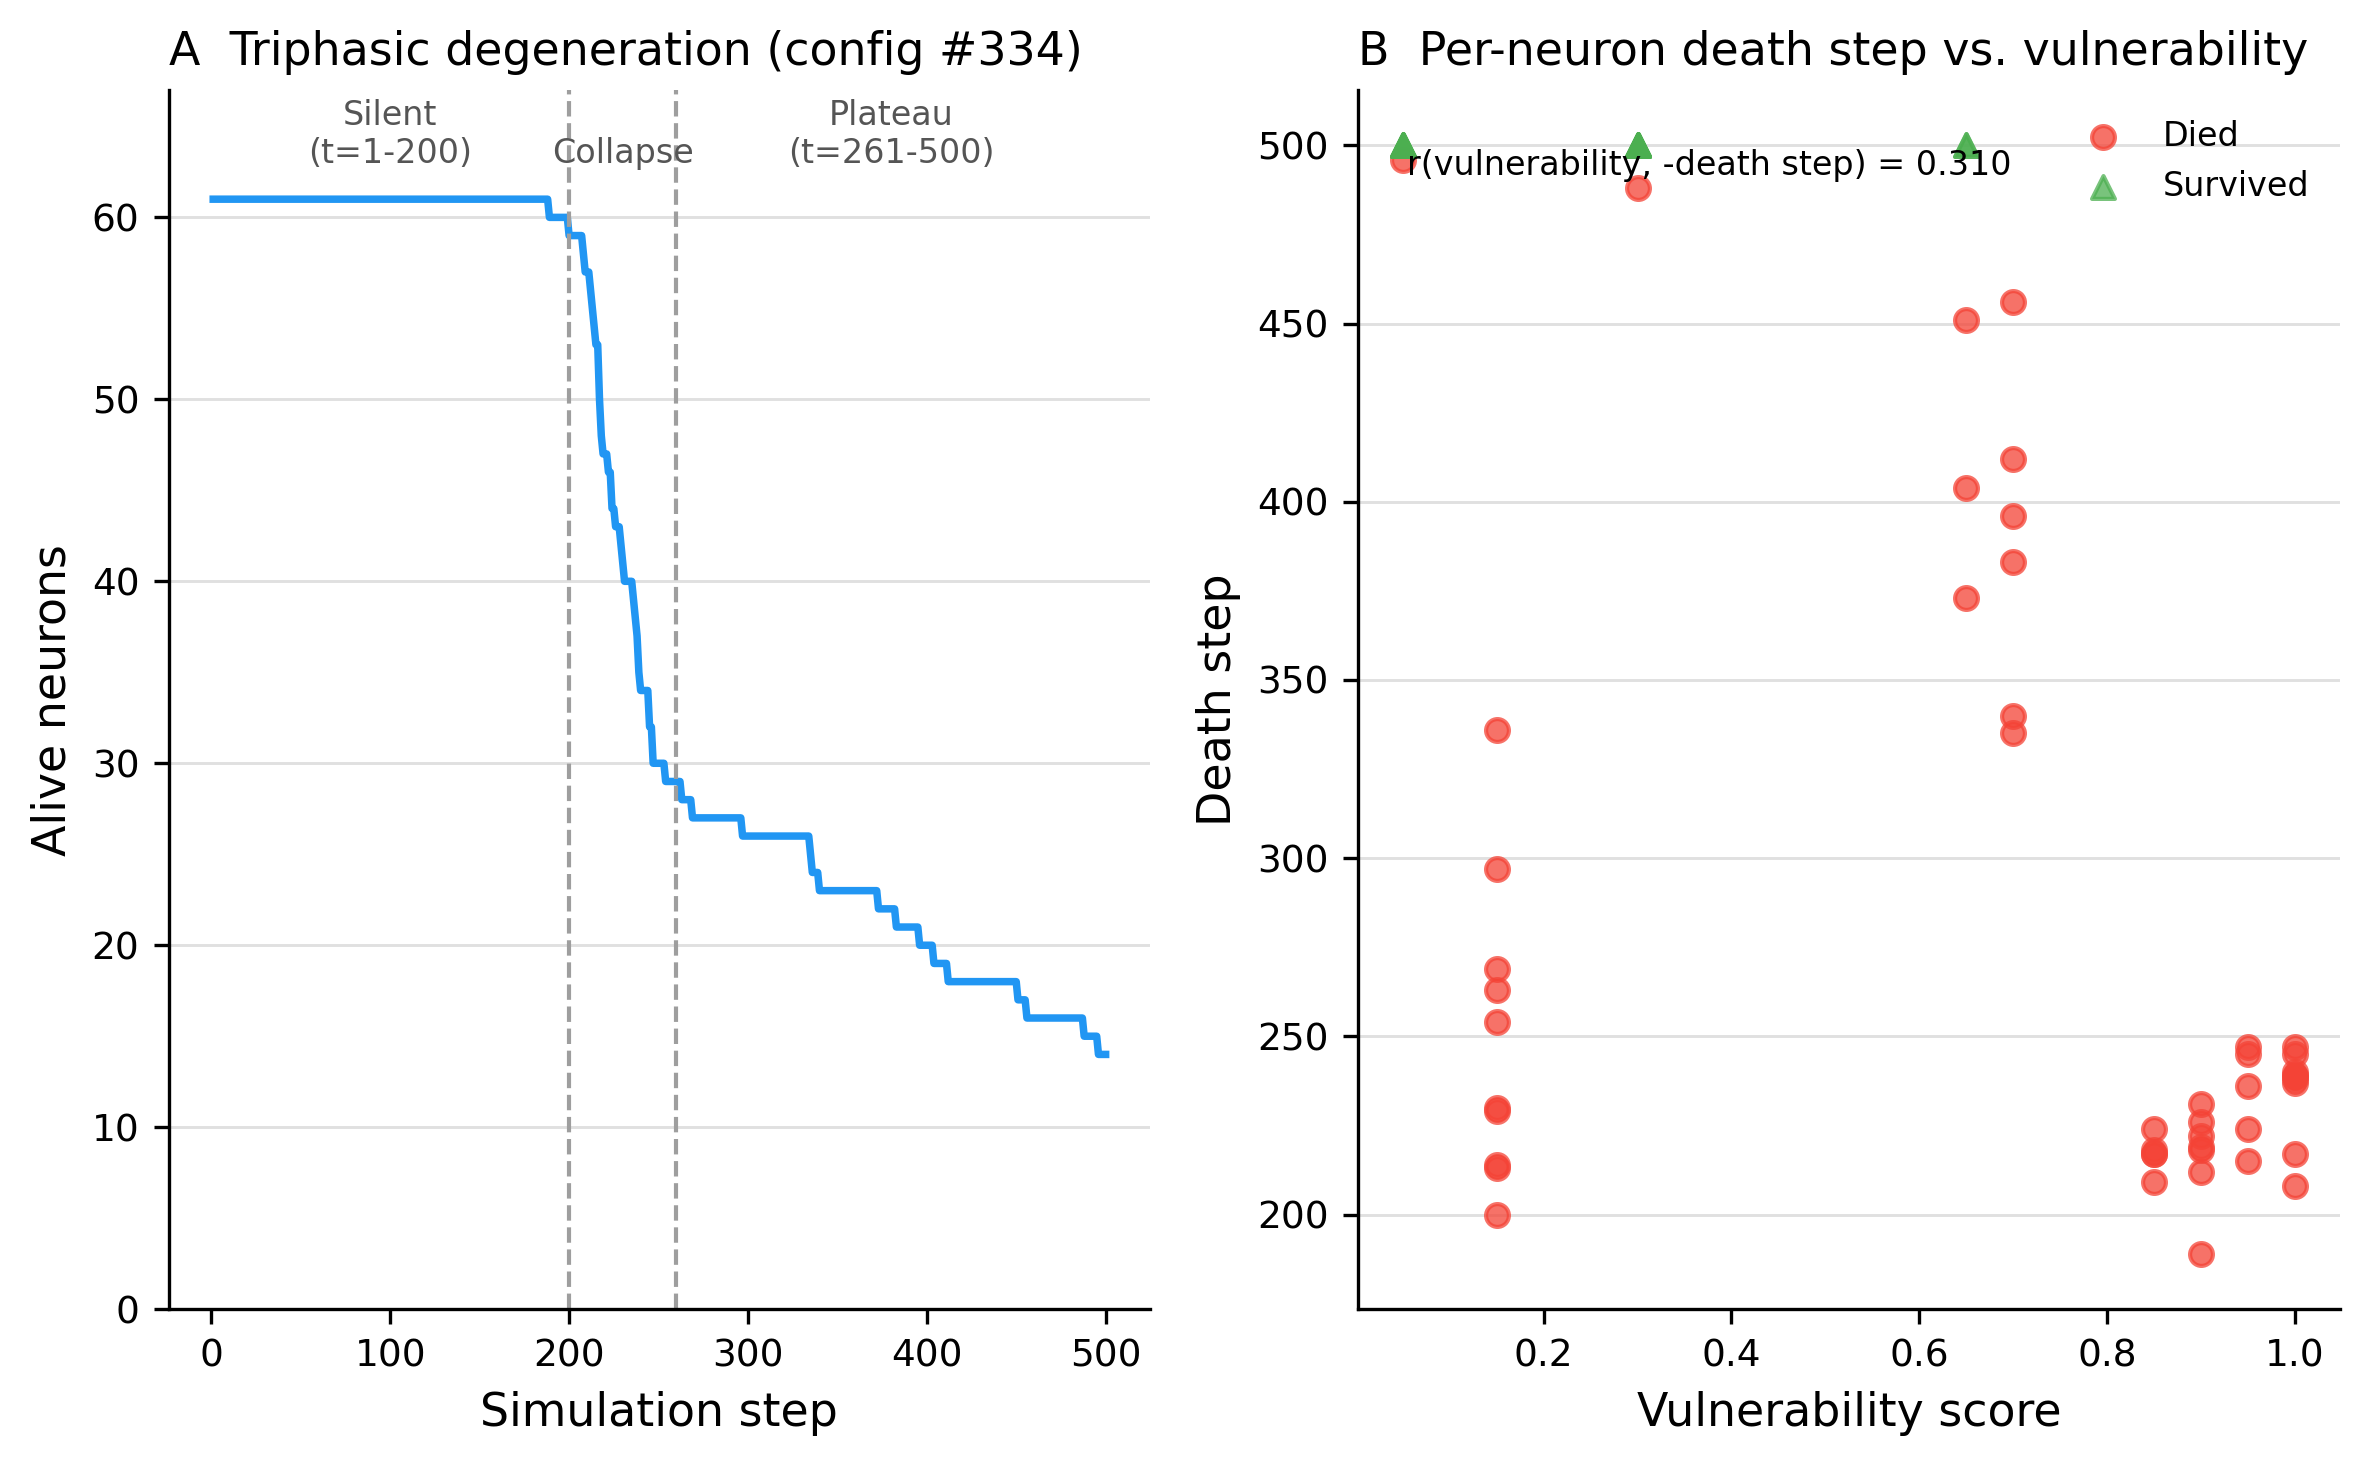
\includegraphics[width=0.9\textwidth]{figures/fig2_config334_triphasic.png}
\caption{Config~\#334 triphasic degeneration pattern showing the silent phase (steps~0--200),
rapid collapse phase (steps~200--280), and arrested plateau of 10 survivors (steps~280--500).}
\label{fig:triphasic}
\end{figure}

\textbf{Top-ranked configurations} for therapy and subtype analysis were selected by maximising
both the depth of the silent phase ($\geq 10$ alive at step~200) and the severity of collapse
($\leq 50$ alive at step~500), yielding a score of $(\text{alive}_{200} - 10 + 50 -
\text{alive}_{500})/40$. Config~\#334 achieved the maximum score of 1.0.

\subsection{Phase~6: Therapeutic window --- aggregation suppression dominates}

Five therapy classes were tested across 10 critical-regime environments (the top-10 Phase-5
configurations) using 500 randomly sampled therapy configurations each. The scoring composite
weighted tipping delay (0.30), functional duration gain (0.30), plateau gain (0.25), and
key-neuron survival (0.15).

Aggregation suppression (\texttt{agg\_sup}) dominated across every metric (Table~\ref{tab:therapy}).
The best configuration achieved a composite score of 0.686 (strength~$= 0.855$,
start\_t~$= 13$), delaying the tipping point by 76.4 steps, extending functional survival by
39.7 steps, and increasing plateau survivors by 36.4 neurons. Importantly, at the parameter
level, \texttt{strength} was almost perfectly predictive of score (Pearson $r = 0.923$),
confirming that the degree of suppression --- not nuanced timing within the tested range ---
was the primary determinant.

\begin{table}[H]
\centering
\caption{Therapy class performance comparison.}
\label{tab:therapy}
\begin{tabularx}{\textwidth}{llrrrX}
\toprule
\textbf{Class} & \textbf{Best score} & \textbf{Tip delay} & \textbf{Func gain}
  & \textbf{Plat gain} & \textbf{Mechanism}\\
\midrule
\texttt{agg\_sup}   & 0.686 & $+76.4$ & $+39.7$ & $+36.4$ & Aggregation suppression\\
\texttt{adaptive}   & 0.453 & $+50.3$ & $+39.7$ & $+22.0$ & Biomarker-triggered agg+ATP\\
\texttt{glut\_sup}  & 0.082 & $+2.0$  & $+4.6$  & $+1.9$  & Glutamate suppression\\
\texttt{astro\_sup} & 0.063 & $+3.7$  & $+3.5$  & $+1.3$  & Astrocyte toxin clearance\\
\texttt{met\_sup}   & 0.034 & $-0.7$  & $-0.9$  & $-0.1$  & ATP recovery boost\\
\bottomrule
\end{tabularx}
\end{table}

The near-zero efficacy of \texttt{met\_sup} and \texttt{glut\_sup} is mechanistically consistent
(see Section~\ref{sec:escape}): both the mitochondrial and glutamate pathways are gated by
aggregation-driven ATP depletion; interventions targeting downstream nodes cannot compensate for
ongoing upstream pathology.

The adaptive biomarker-triggered strategy achieved intermediate performance (score 0.453),
exploiting the triphasic structure by intervening at the silent-to-collapse transition boundary
--- but it requires accurate early-stage biomarker detection and achieves lower plateau gains
than direct high-strength suppression.

\subsection{Phase~7A/7B: Rigorous falsification of tipping points}

\subsubsection{Ablation study (Phase~7A)}

Config~\#334 was re-run six times, each disabling exactly one mechanism. Results were
unambiguous: removing aggregation seeding completely eliminated the tipping point, extending
first-death step by 279 steps (to step~500) and leaving 60/61 neurons alive. No other single
ablation --- including removal of ATP collapse, glutamate/calcium/ROS cascade, astrocyte
clearance, or irreversibility --- changed the survival curve detectably (tipping step unchanged,
plateau unchanged). The mechanistic model diverged sharply from random-noise replacement (which
delayed tipping by 239 steps but produced a gradual rather than sharp collapse).

The conclusion is clear: \textbf{aggregation seeding is the sole load-bearing mechanism} in
config~\#334. The downstream cascade (ATP $\to$ glutamate $\to$ calcium $\to$ ROS $\to$
oxidative feedback) provides amplification but is not rate-limiting, because in config~\#334
the \texttt{glutamateSensitivity} is extremely low (0.00072), keeping the glutamate pathway
near-silent regardless of ATP status.

\subsubsection{Null model and strict criterion (Phase~7B)}

A null model replaced all mechanistic equations with independent per-neuron random health
decrements, producing comparable overall mortality (mean 29/61 alive at $t = 500$) without any
coupling between neurons. The original single-threshold criterion classified 44/100 null-model
runs as exhibiting tipping points --- a 44\% false-positive rate unacceptably high for
scientific claims.

The decisive discriminator is \textbf{spatial coherence}: in the mechanistic model, aggregation
spreads preferentially via synaptic connections to high-vulnerability neurons, producing a
strong correlation between a neuron's vulnerability score and how early it dies (Pearson
$r > 0.30$ in genuine configs, mean $r = 0.56$ in the 247 confirmed cases). In the null model,
death order is independent of vulnerability (mean $r = -0.01$, all 100 runs below $r = 0.11$).
Adding this as criterion C2 reduced the null false-positive rate to exactly 0/100 (0\%) while
retaining 247/382 (64.7\%) critical configurations as genuine (Figure~\ref{fig:falsification}).

\begin{figure}[H]
\centering
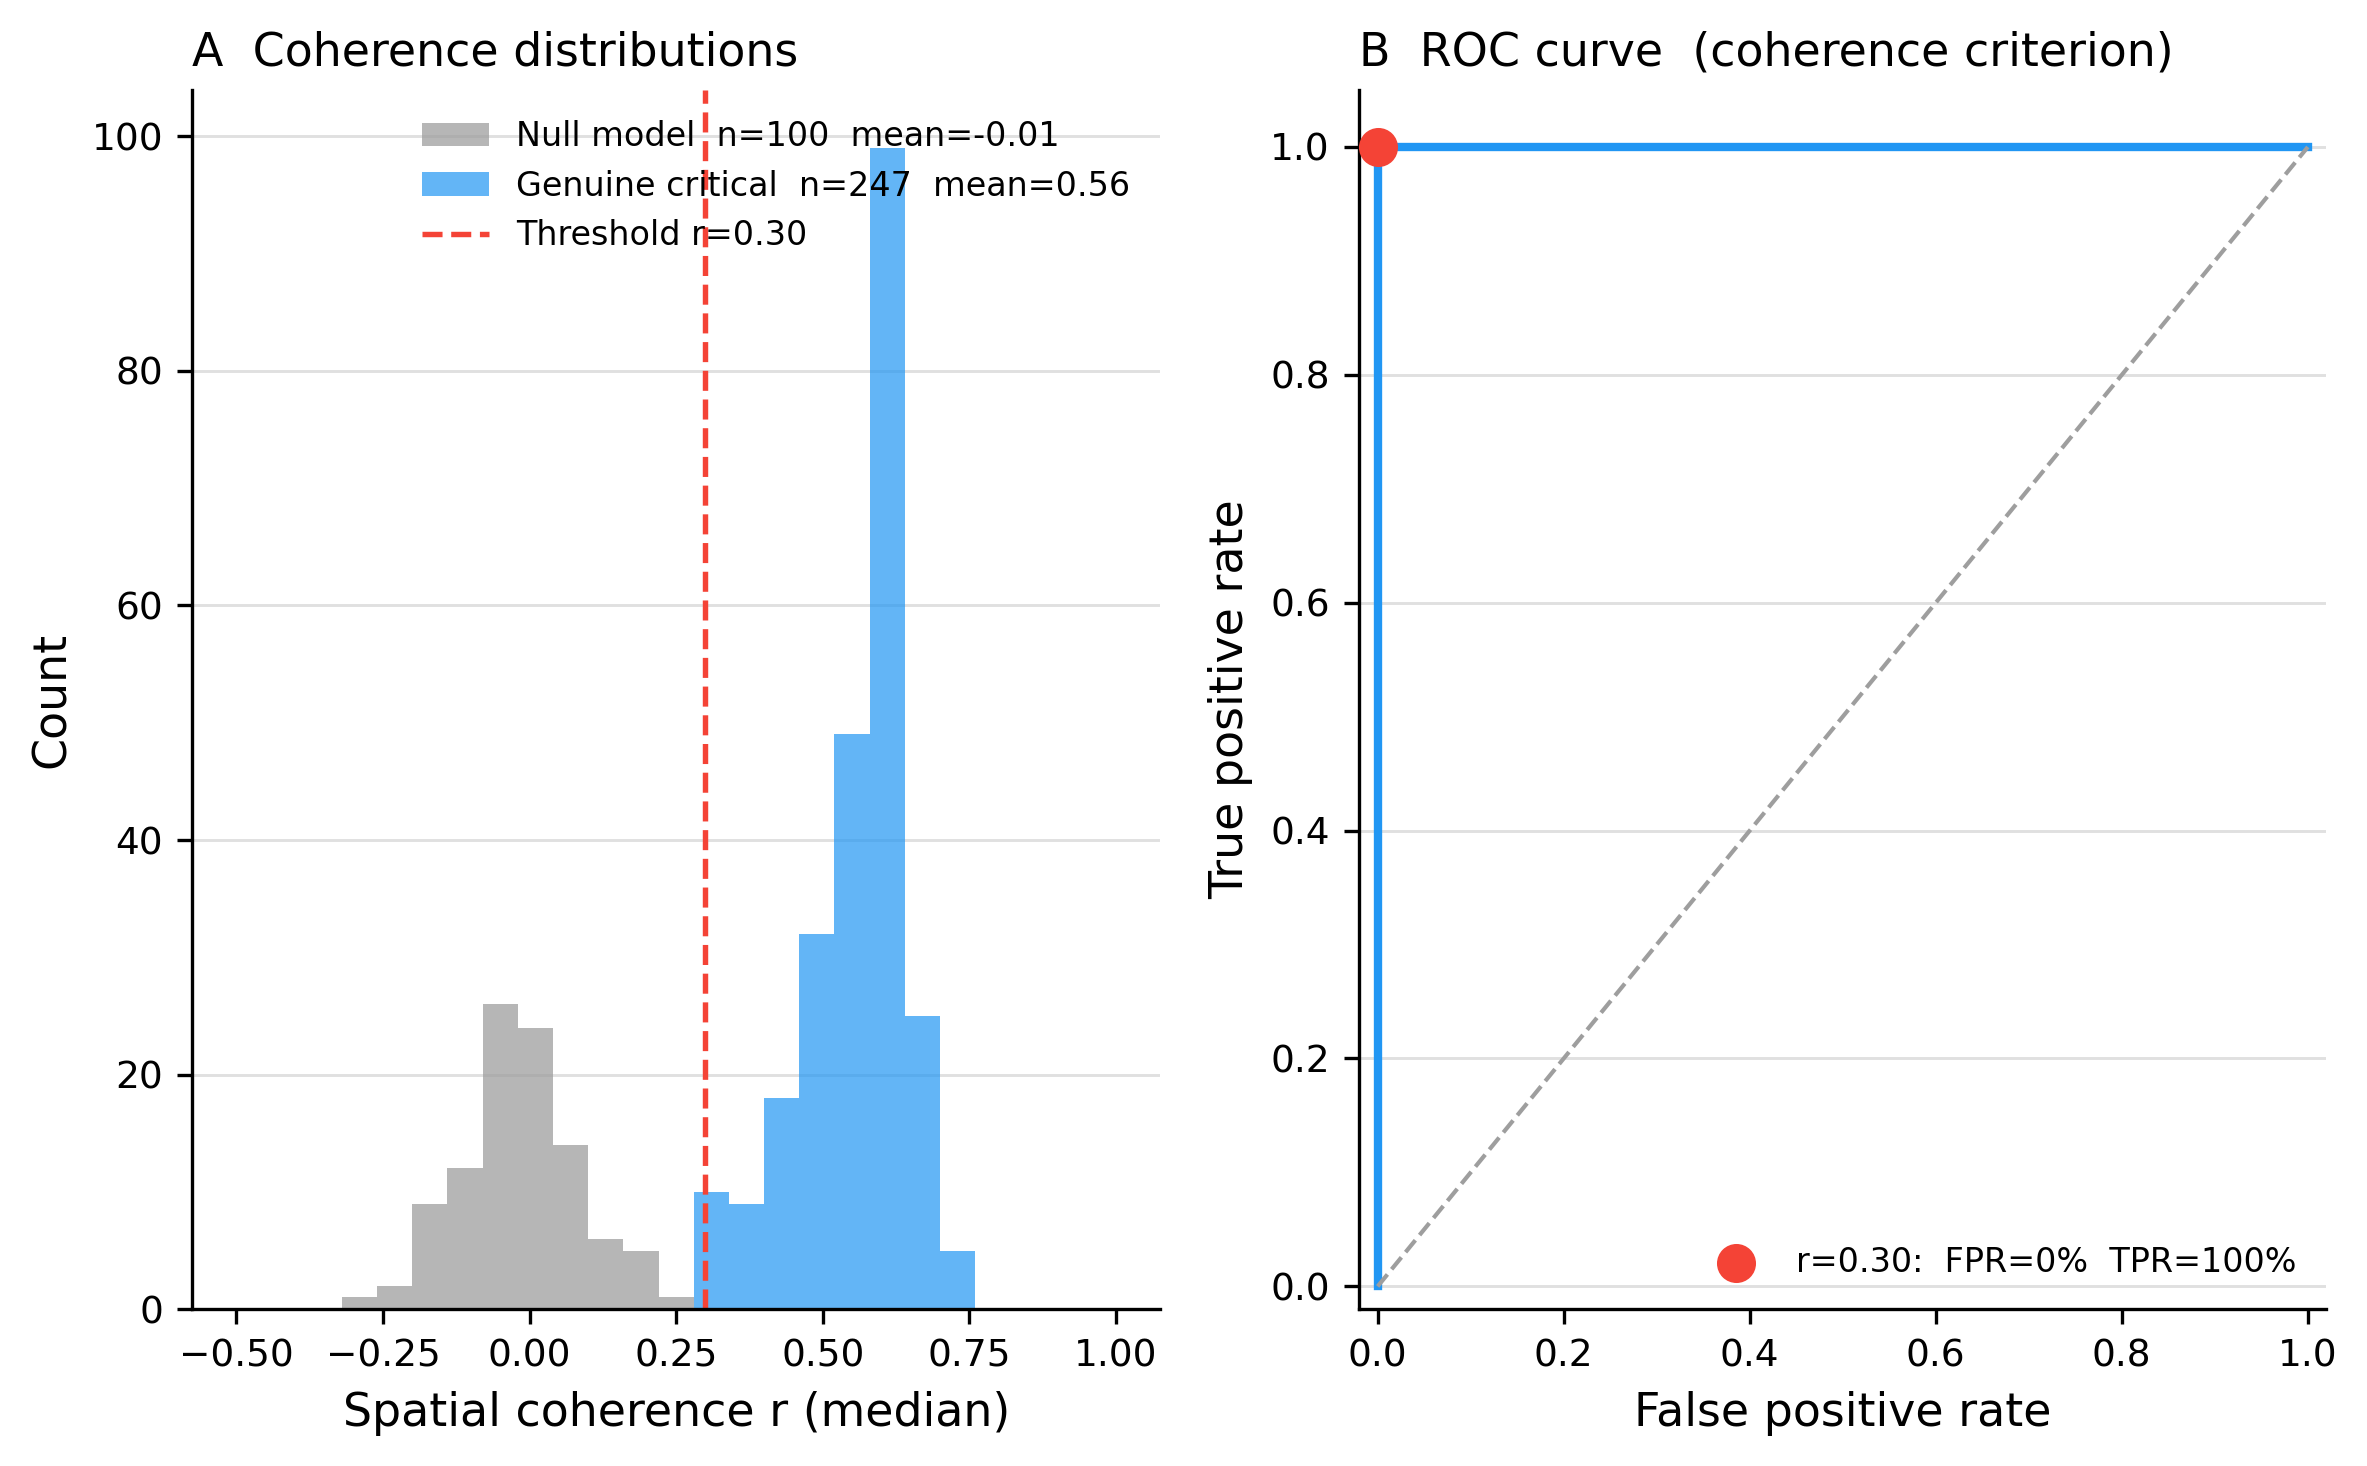
\includegraphics[width=0.9\textwidth]{figures/fig3_null_model_falsification.png}
\caption{Null model falsification. The strict three-part criterion (slope, spatial coherence,
silent phase) reduces the false-positive rate from 44\% to 0\% while retaining 64.7\% of
critical configurations as genuine.}
\label{fig:falsification}
\end{figure}

\begin{table}[H]
\centering
\caption{Tipping criterion outcomes before and after falsification.}
\label{tab:falsification}
\begin{tabular}{lcc}
\toprule
\textbf{Dataset} & \textbf{Original criterion} & \textbf{Strict criterion}\\
\midrule
Phase~5 critical (382)  & 382/382 (100\%)  & 247/382 (64.7\%)\\
Phase~6 therapies (10)  & 10/10 (100\%)    & 7/10 (70\%)\\
Null model (100)        & 44/100 (44\%)    & 0/100 (0\%)\\
\bottomrule
\end{tabular}
\end{table}

\subsection{Phase~7C: Topology dependence of criticality}

The same biophysical parameters (10 critical-regime configurations) were applied to five
different 61-node network topologies: the empirical \textit{C.~elegans} motor connectome,
Erd\H{o}s-R\'{e}nyi random graphs (ER), Barab\'{a}si-Albert scale-free networks (BA),
Watts-Strogatz small-world networks (WS), and degree-sequence-preserved random shuffles of the
\textit{C.~elegans} graph. All networks maintained 127 directed edges; 10 random instances were
generated for each synthetic type.

\textbf{Topology profoundly affects tipping point emergence.} The genuine tipping rate under the
Phase~7B criterion varied from 0\% (BA) to 100\% (\textit{C.~elegans}):

\begin{table}[H]
\centering
\caption{Topology dependence of genuine tipping rates.}
\label{tab:topology}
\begin{tabular}{p{4cm}ccc}
\toprule
\textbf{Topology} & \textbf{Genuine rate} & \textbf{Mean coherence $r$}
  & \textbf{Mean plateau}\\
\midrule
\textit{C.~elegans} (biological)   & 1.000 & 0.582 & 11.3\\
Watts-Strogatz (small-world)       & 0.780 & 0.423 & 4.3\\
Degree-preserved shuffle           & 0.730 & 0.378 & 11.9\\
Erd\H{o}s-R\'{e}nyi (random)      & 0.480 & 0.295 & 3.8\\
Barab\'{a}si-Albert (scale-free)   & 0.000 & $-0.104$ & 2.5\\
\bottomrule
\end{tabular}
\end{table}

The Barab\'{a}si-Albert network's complete resistance to genuine tipping is mechanistically
interpretable: scale-free hub topology provides load-bearing redundancy, distributing damage
broadly rather than concentrating it in ordered sequences through high-vulnerability nodes.
The \textit{C.~elegans} wiring, with its moderate degree variance and high modularity, instead
channels aggregation spread through anatomically defined vulnerability gradients, producing the
strongest spatial coherence of any topology tested (Figure~\ref{fig:topology}).

\begin{figure}[H]
\centering
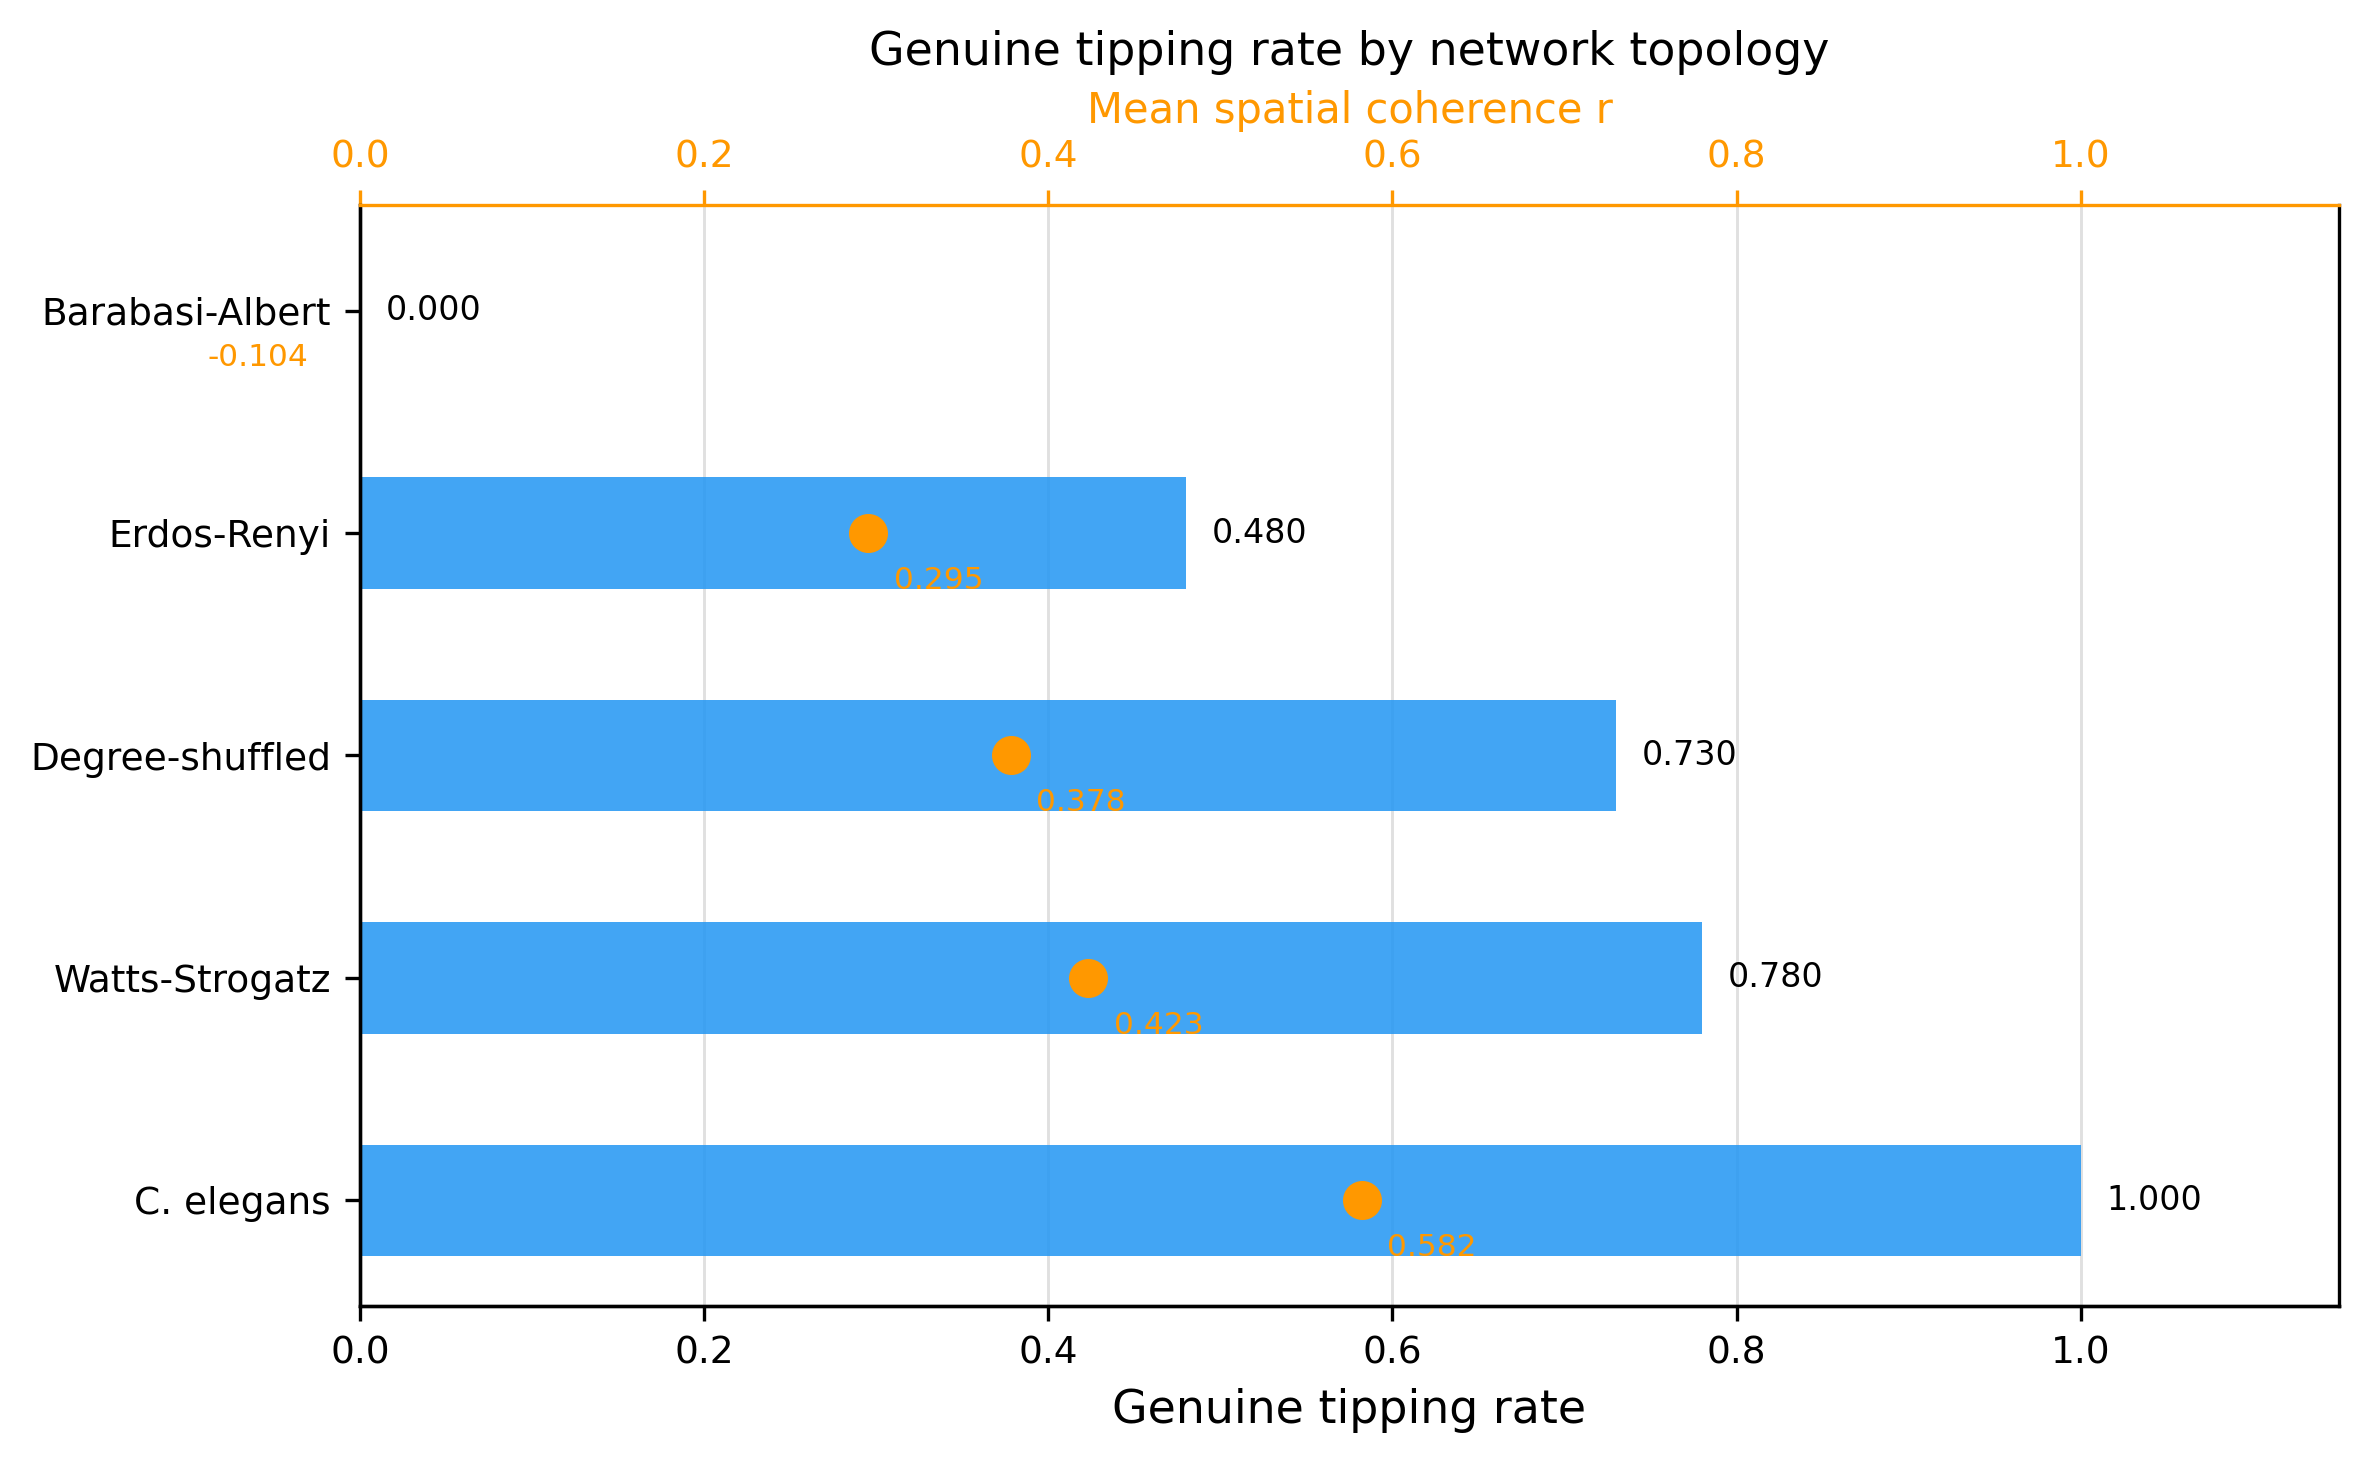
\includegraphics[width=0.9\textwidth]{figures/fig4_topology_dependence.png}
\caption{Topology dependence of genuine tipping rates across five network architectures.
\textit{C.~elegans} biological wiring achieves 100\% genuine tipping rate while
Barab\'{a}si-Albert scale-free networks achieve 0\%.}
\label{fig:topology}
\end{figure}

\textbf{Therapy dynamics are topology-independent.} Despite striking topology dependence in
untreated degeneration, aggregation suppression therapy (strength~$= 0.855$, start\_t~$= 13$)
achieved 100\% prevention (tipping pushed beyond step~300) in all five topologies. This
demonstrates that the therapeutic mechanism operates primarily via Tier~1 (biochemical
suppression of aggregation growth) rather than through topology-specific load redistribution.

\subsection{Phase~7D: Disease escape analysis and the two-tier model}
\label{sec:escape}

A critical test of model validity is whether the disease can escape aggregation suppression
through alternative pathways. Three escape scenarios were tested:

\begin{itemize}
\item \textbf{Escape~1 (mitochondrial/ATP)}: aggregation growth disabled, mitochondrial
fragility pathway active.
\item \textbf{Escape~2 (glutamate excitotoxicity)}: aggregation growth disabled, glutamate
sensitivity tripled.
\item \textbf{Escape~3 (load redistribution)}: all biochemistry disabled, pure topological
cascade.
\end{itemize}

\textbf{Biochemical escapes fail completely.} Escapes~1 and 2 each produced genuine tipping
rate $= 0.000$ across all 10 configurations and 5 seeds. The mechanistic reason is identical
for both: with aggregation growth suppressed, intracellular ATP remains near 1.0, preventing
the ATP depletion event that gates glutamate release. With the gate closed, neither enhanced
mitochondrial fragility nor tripled glutamate sensitivity can activate the excitotoxic cascade.

\textbf{Topological escape is genuine and catastrophic.} Escape~3 (pure load redistribution,
no biochemistry) produced genuine tipping rate~$= 1.000$, spatial coherence $r = 0.914$, and a
near-total plateau of 1.0 survivor --- more destructive than the full biochemical model
(${\sim}10$ survivors). Once enough neurons die to shift load onto their synaptic partners, the
cascade becomes self-sustaining even without any protein aggregation dynamics.

This result establishes a \textbf{two-tier disease model}:

\begin{itemize}
\item \textbf{Tier~1} (biochemical cascade): aggregation seeding $\to$ ATP collapse $\to$
excitotoxicity. Therapy-sensitive. Aggregation suppression completely silences this tier.
\item \textbf{Tier~2} (topological cascade): load redistribution among dying neurons.
Therapy-insensitive if initiated after sufficient neuron loss. Operates independently of
aggregation, ATP, and all biochemistry.
\end{itemize}

The practical implication is that therapy must prevent Tier~1 from producing the death threshold
that triggers autonomous Tier~2 amplification.

\subsection{Phase~8: Two-tier mechanism --- cascade initiation analysis}

Config~\#334 was examined in granular detail to characterise the transition from biochemical
(Tier~1) to topological (Tier~2) propagation.

\textbf{Death sequence and network properties.} The first 10 neurons to die in the canonical
run (seed~434, no therapy) were exclusively motor neurons: DD1 (step~201), DA2 (206), DB1
(208), DD2 (210), DD3 (215), VA1 (219), VA2 (221), VD1 (225), VD2 (225), DD4 (228). All had
vulnerability scores 0.65--1.00. This demonstrates that Tier~1 targets neurons by biochemical
vulnerability, not topological centrality.

Tier~2 was operationally defined as activation when cumulative deaths exceed 5 (a threshold
validated by comparing cascade rates before and after). Under baseline conditions, Tier~2
activated at step~220, triggering 32 additional deaths in the subsequent 100 steps.

\textbf{Surgical protection experiments.} Six neuron-protection groups (10$\times$ health-loss
reduction, no aggregation suppression) were tested:

\begin{table}[H]
\centering
\caption{Surgical protection experiment results. Random control (50 repeats, 3 neurons each):
mean plateau $= 12.6 \pm 0.5$.}
\label{tab:protection}
\begin{tabular}{lp{3.5cm}ccc}
\toprule
\textbf{Group} & \textbf{Protected neurons} & \textbf{Plateau}
  & \textbf{Tier~2 step} & \textbf{Above random?}\\
\midrule
Baseline      & ---              & 11.0 & 220 & ---\\
A (first 1)   & DD1              & 12.0 & 220 & No\\
B (first 3)   & DD1, DA2, DB1    & 14.0 & 220 & Yes\\
C (first 5)   & DD1--DD3         & 16.0 & 226 & Yes\\
D (DA6, AVDL) & Hub neurons      & 13.0 & 220 & No\\
E (top vuln.) & DA1--DA3         & 14.0 & 221 & Yes\\
F (top degree)& AVAL, AVAR, AVBL & 14.0 & 220 & Yes\\
Full therapy  & ---              & 53.0 & 485 & ---\\
\bottomrule
\end{tabular}
\end{table}

No group approached full therapy (plateau~53). Tier~2 was delayed by at most 6 steps (Group~C)
versus 265 steps by full therapy. \textbf{Only blocking Tier~1 (aggregation suppression)
prevents the deaths that seed Tier~2.} Full therapy (start\_t~$= 13$) delayed first death by
184 steps (step~201 $\to$ 385), which in turn delayed Tier~2 activation by 265 steps
(step~220 $\to$ 485), producing a plateau of 53 survivors versus 11 in the untreated model.

\subsection{Phase~9: Therapeutic boundary --- a linear phase diagram}

The minimal effective aggregation suppression was mapped systematically for config~\#334 across
a $9 \times 11$ grid: nine therapy strengths (0.10--0.90) $\times$ eleven start times ($t =
0$--250), with five seeds per grid point (495 total runs, 500 steps each). Each grid point was
classified as prevention (tipping rate $= 0$), mixed ($0 <$ rate $< 1$), delay (tipping
delayed $> 30$ steps), partial (10--30 steps), or ineffective ($< 10$ steps).

\textbf{A sharp linear therapeutic boundary.} The boundary between the prevention/mixed and
delay/ineffective zones in (strength, start\_t) space was well-described by a linear fit
(Figure~\ref{fig:phasediag}):

\begin{equation}
\mathrm{max\_start\_t} = 425 \times \text{strength} - 237 \quad (R^2 = 0.980)
\label{eq:boundary}
\end{equation}

\begin{figure}[H]
\centering
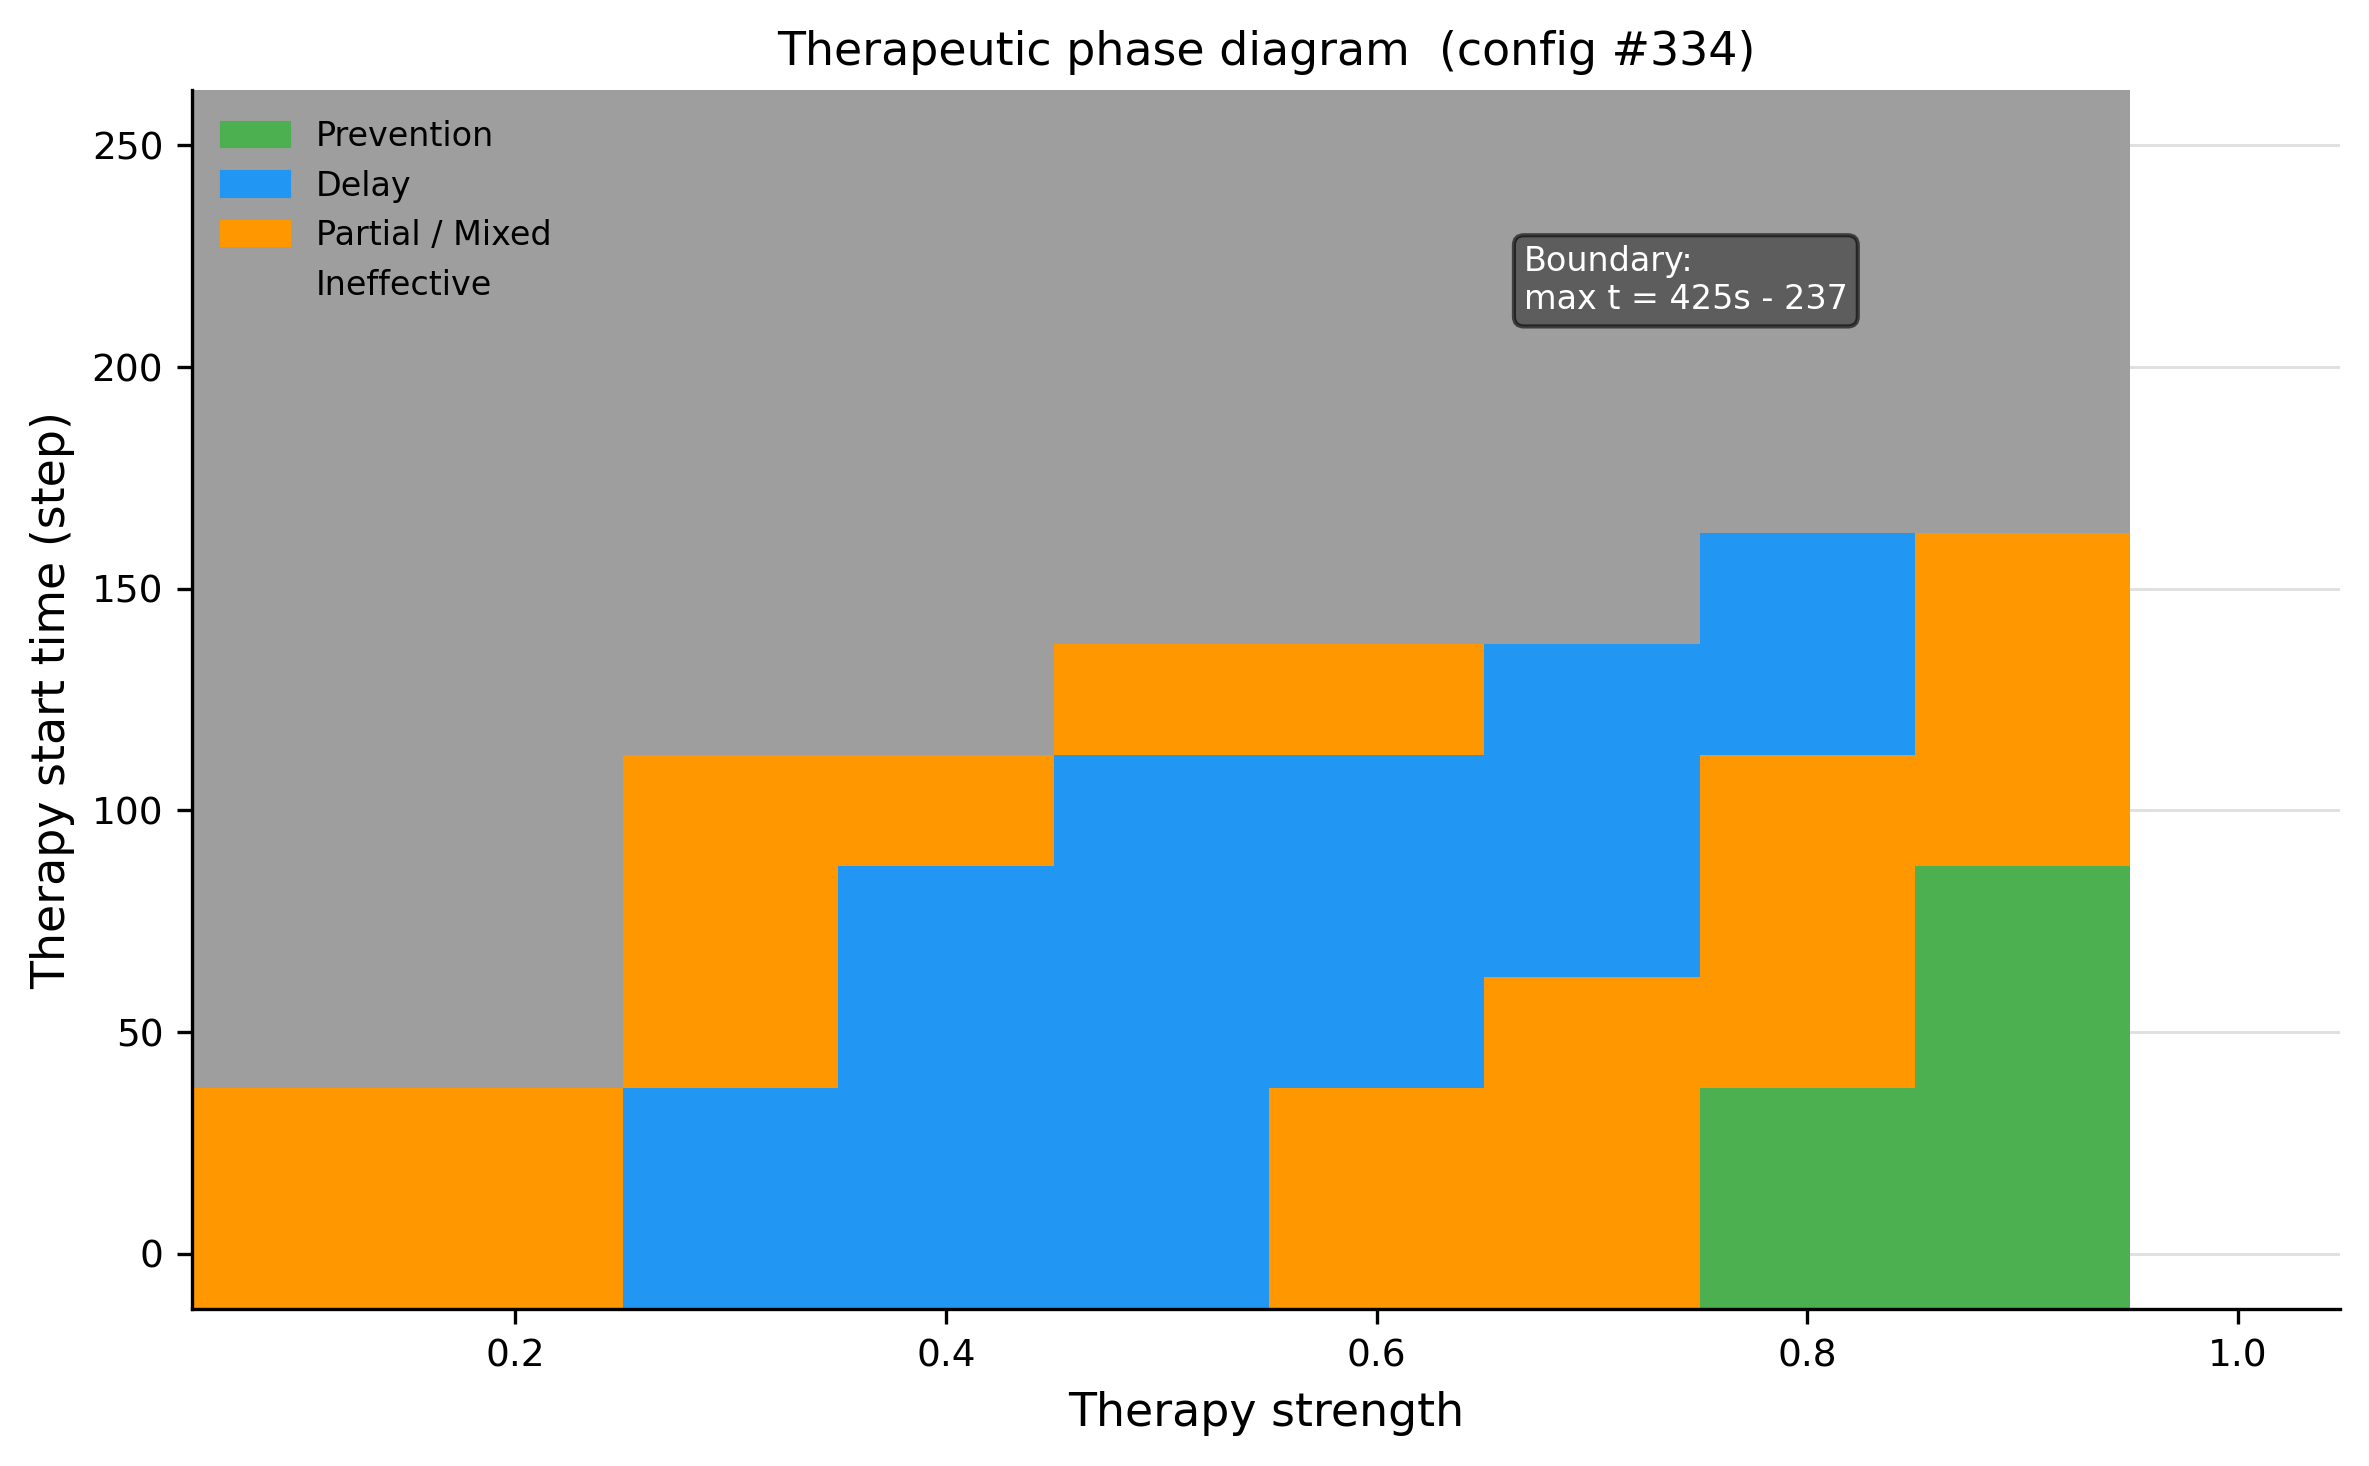
\includegraphics[width=0.9\textwidth]{figures/fig5_phase_diagram.png}
\caption{Therapeutic phase diagram for config~\#334. The sharp linear boundary
$\mathrm{max\_start\_t} = 425 \times \text{strength} - 237$ ($R^2 = 0.980$) separates
prevention (blue) from delay/ineffective (red) zones.}
\label{fig:phasediag}
\end{figure}

\begin{table}[H]
\centering
\caption{Therapeutic window as a function of therapy strength. \textit{Calibration: 200
simulation steps $\approx$ 15 months pre-symptomatic; 1 step $\approx$ 2.25 days. Illustrative
only; not derived from biological measurements.}}
\label{tab:window}
\begin{tabular}{ccc}
\toprule
\textbf{Strength} & \textbf{Latest prevention start} & \textbf{Approx.\ pre-clinical window}\\
\midrule
0.60 & $t = 25$  & Pre-symptomatic, very early\\
0.70 & $t = 50$  & Pre-symptomatic, early\\
0.80 & $t = 100$ & Pre-symptomatic, ${\sim}$7 months\\
0.90 & $t = 150$ & Pre-symptomatic, ${\sim}$11 months\\
\bottomrule
\end{tabular}
\end{table}

No prevention was achieved at any strength for start times $\geq 175$ steps. The relationship
between strength and window width is linear, not asymptotic: there is no ``good enough'' strength
that allows indefinitely late intervention.

\textbf{Comparison with ALS clinical observations.} The model's prediction that moderate
suppression (${\sim}$60--70\% reduction, consistent with published ASO efficacy ranges) requires
initiation well before symptom onset is qualitatively consistent with the ATLAS trial finding
that pre-symptomatic tofersen intervention delayed phenoconversion \citep{benatar2023}, while
post-symptomatic intervention in the VALOR trial \citep{miller2022} produced more modest
effects. We stress that this correspondence is qualitative and does not constitute model
validation.

\subsection{Phase~10: Boundary robustness across 20 disease configurations}

The Phase~9 boundary was tested for generalisability across the top-20 genuine critical
configurations from Phase~7B, using a $9 \times 9$ strength $\times$ start\_t grid with 3
seeds per point and 500 steps (4,860 total runs).

Seventeen of twenty configurations produced measurable linear boundaries; three (IDs~241, 329,
87) showed flat boundaries (prevention achievable at any start time, slope~$\approx 0$) ---
indicating configurations mild enough that even late, weak therapy prevents collapse.

For the 17 configs with measurable boundaries:
\begin{itemize}
\item Slope: mean $= 252 \pm 120$ (range 59--500)
\item Intercept: mean $= -107 \pm 117$
\item $R^2$: mean $= 0.832$, with 65\% of configs achieving $R^2 > 0.90$ (Figure~\ref{fig:boundary})
\end{itemize}

\begin{figure}[H]
\centering
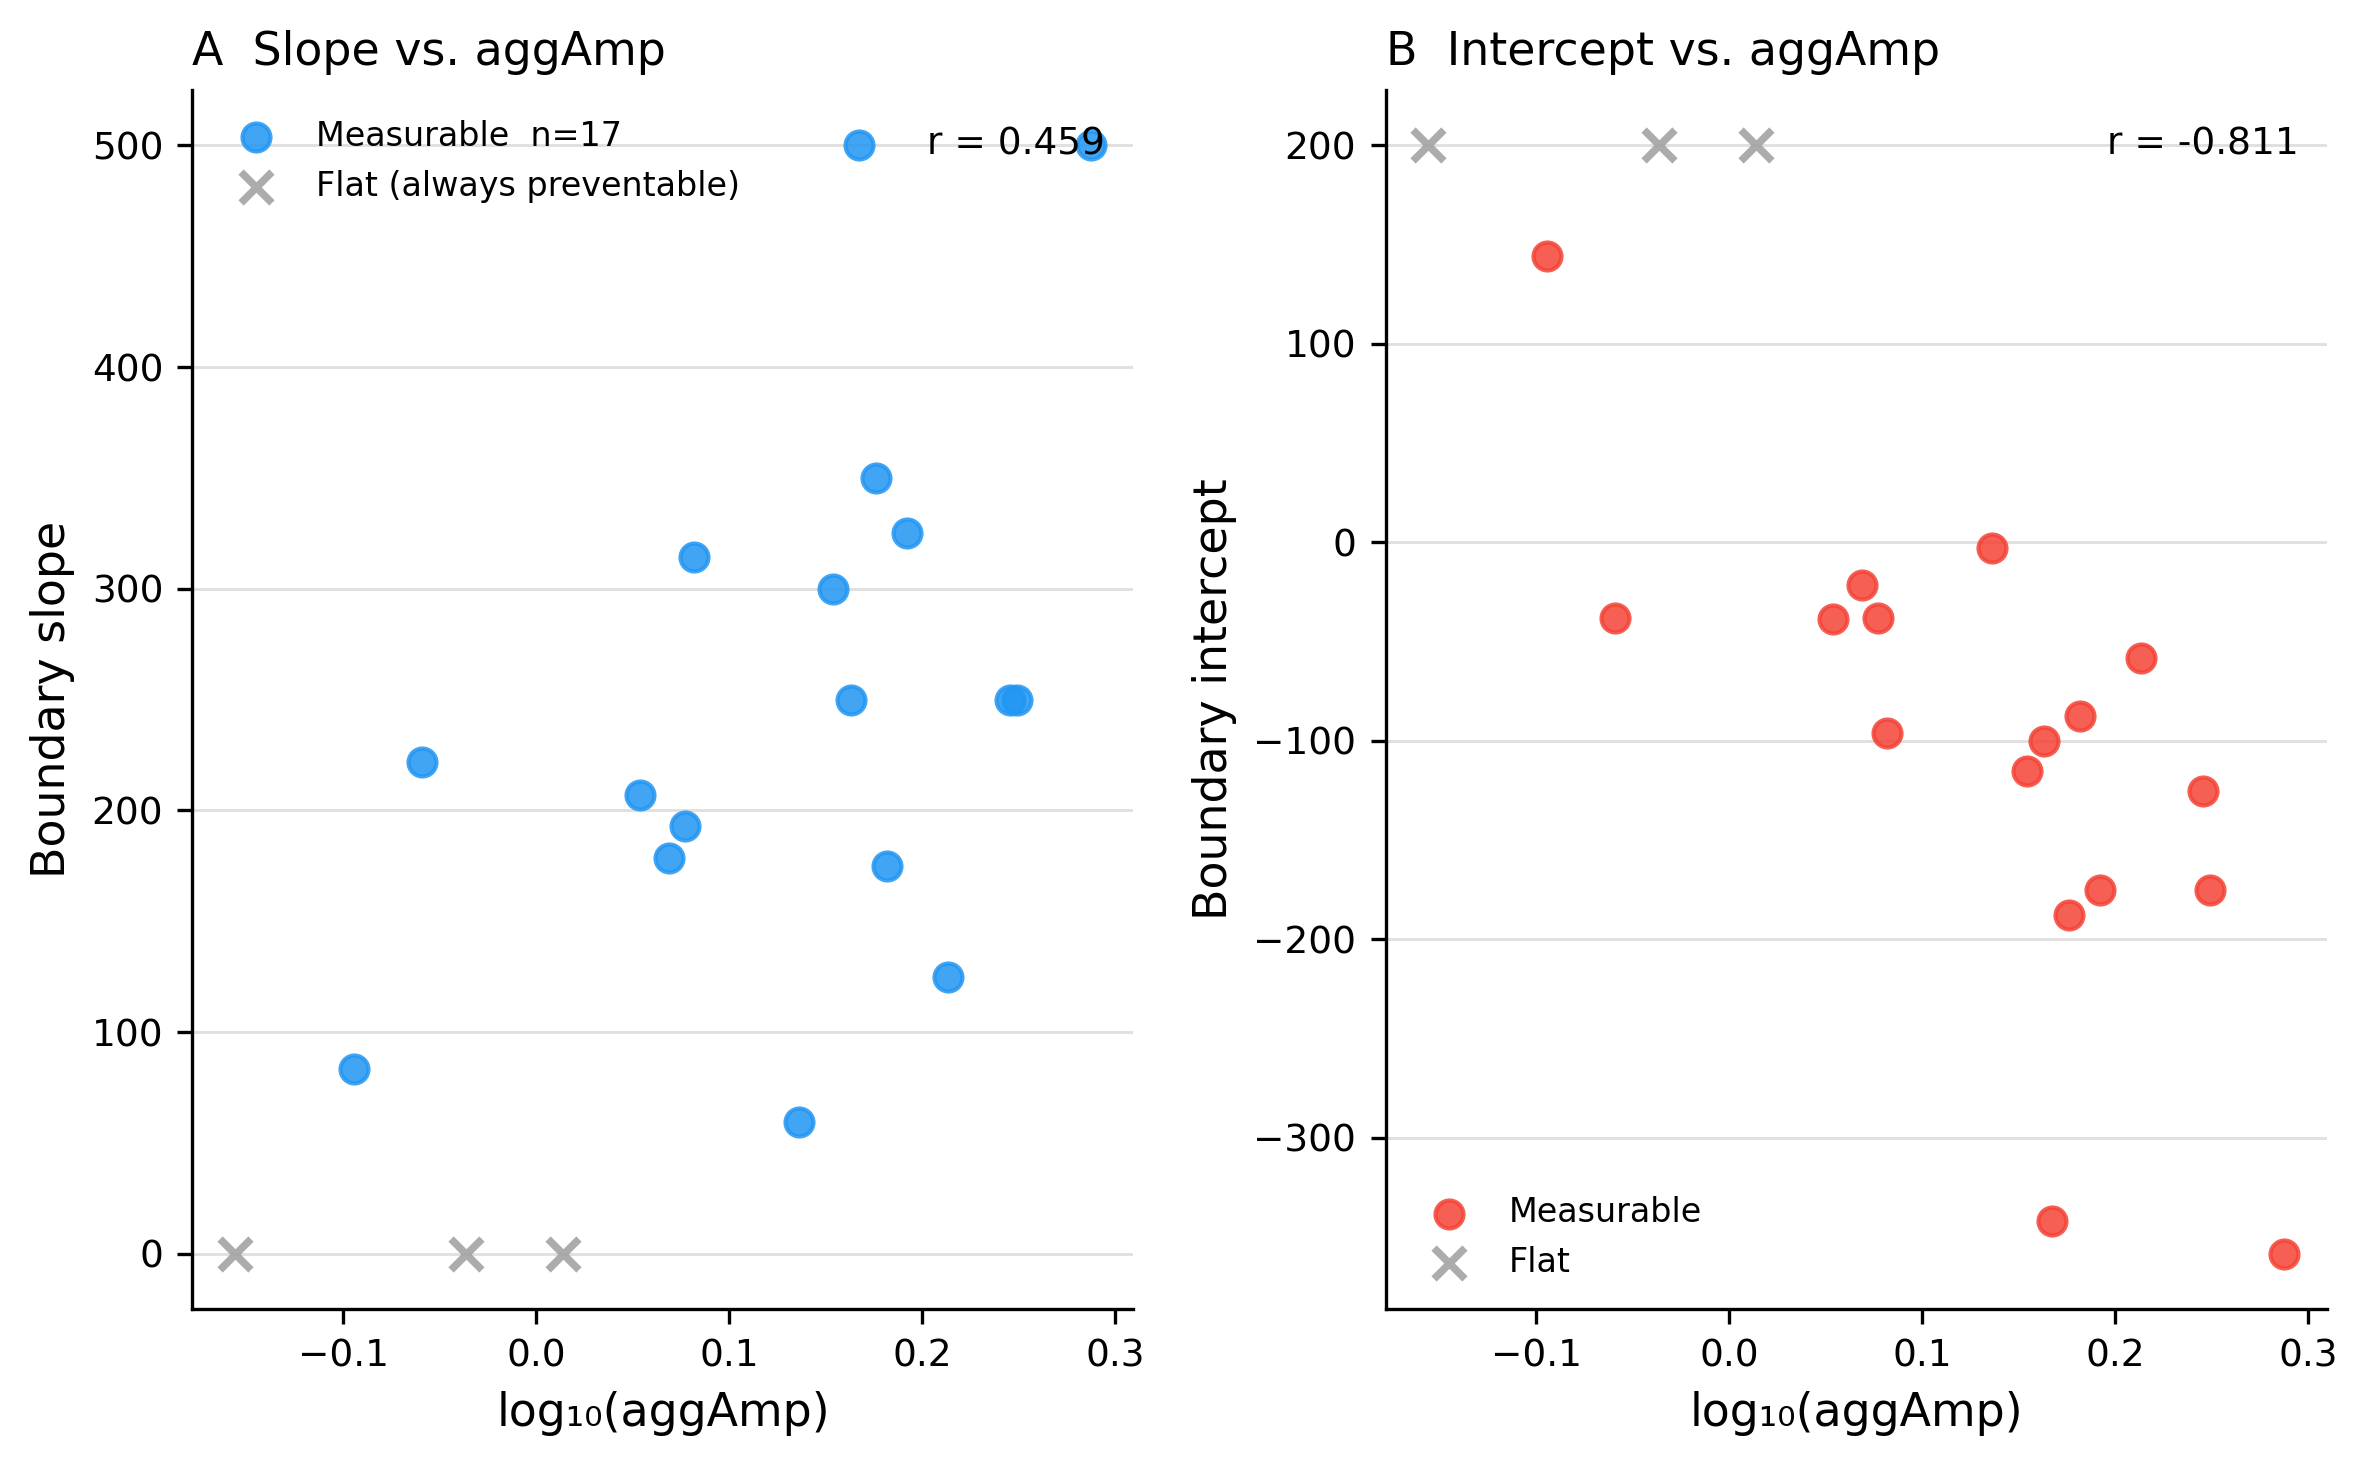
\includegraphics[width=0.9\textwidth]{figures/fig6_boundary_robustness.png}
\caption{Therapeutic boundary robustness across 20 disease configurations. Mean slope
$= 252 \pm 120$, mean $R^2 = 0.832$. The index config~\#334 (slope~$= 350$) falls within
one standard deviation of the population mean.}
\label{fig:boundary}
\end{figure}

\textbf{Aggregation amplitude predicts boundary position.} Among all seven parameters,
\texttt{aggregationAmplification} was the strongest predictor of boundary shape, with Pearson
$r = +0.645$ for slope and $r = -0.811$ for intercept.

\textbf{A conservative therapeutic boundary.} The population mean minus one standard deviation
gives a conservative estimate applicable to approximately 84\% of configurations:

\begin{equation}
\mathrm{max\_start\_t}_{\text{conservative}} = 132 \times \text{strength} - 224
\label{eq:conservative}
\end{equation}

At the clinically relevant strength of 0.80, this conservative boundary implies therapy must
begin before disease initiation (negative start time), indicating that highly aggressive disease
subtypes may have windows that close before biomarker-detectable onset.

\subsection{Phase~11/12: Disease subtypes from unsupervised clustering}

\subsubsection{Phase~11: Subtype structure in the top-20 configurations}

K-means clustering ($K = 2, 3, 4$) of the top-20 critical configurations using five features
(tipping step, plateau, boundary slope, boundary intercept, \texttt{aggregationAmplification})
identified $K = 3$ as optimal (silhouette score 0.43). PCA captured 82.4\% of variance in two
components; PC1 (64.9\%) was dominated by boundary intercept ($-0.53$),
\texttt{aggregationAmplification} ($+0.51$), and boundary slope ($+0.48$) --- all facets of
the same disease-severity axis.

Three subtypes were identified:
\begin{itemize}
\item \textbf{Aggressive} ($n = 3$; IDs~178, 334, 497): \texttt{aggAmp} $\approx 1.64$,
therapy window closes at $t \approx 108$, minimum required strength 0.67.
\item \textbf{Moderate} ($n = 13$): \texttt{aggAmp} $\approx 1.39$, window closes
$t \approx 115$, minimum strength 0.46.
\item \textbf{Mild} ($n = 4$; IDs~87, 235, 241, 329): \texttt{aggAmp} $\approx 0.86$,
window always open (flat boundary), minimum strength 0.10.
\end{itemize}

\subsubsection{Phase~12: Validation on the full 247-configuration dataset}

To test whether the Phase~11 subtype structure was an artefact of pre-selection and to avoid
circular validation, Phase~12 repeated clustering on all 247 genuine critical configurations
using seven simulation-only features (tipping step, plateau survivors, peak decline rate,
silent phase length, spatial coherence $r$, \texttt{aggregationAmplification},
\texttt{mitochondrialFragility}) with no therapy-derived features.

\textbf{PCA on 247 configurations.} PC1 captured 69.7\% of variance, with nearly equal loadings
from tipping step ($-0.44$), silent phase length ($-0.44$), plateau survivors ($-0.43$), peak
decline rate ($+0.42$), and \texttt{aggregationAmplification} ($+0.41$) --- confirming that
these five variables are different manifestations of a single underlying disease-severity axis.
PC2 (19.1\%) was dominated entirely by \texttt{mitochondrialFragility} ($-0.81$), orthogonal
to all other features.

\textbf{Optimal $K = 2$, not $K = 3$.} At the full dataset scale, $K = 2$ provided the best
silhouette score (0.41). The two clusters correspond to a fundamental speed-of-degeneration
split:

\begin{itemize}
\item \textbf{Slow-tipping subtype} ($n = 110$): \texttt{aggAmp} $\approx 1.36$, tipping step
224, plateau 13.1/61 survivors.
\item \textbf{Fast-tipping subtype} ($n = 137$): \texttt{aggAmp} $\approx 5.86$, tipping step
107, plateau 5.3/61 survivors (Figures~\ref{fig:subtype_scatter} and \ref{fig:bootstrap}).
\end{itemize}

These two clusters are better understood as opposite ends of a dynamical continuum rather than
discrete disease categories: the silhouette score of 0.41 indicates substantial overlap at
cluster boundaries, and intermediate configurations exist that could plausibly belong to either
class.

\begin{figure}[H]
\centering
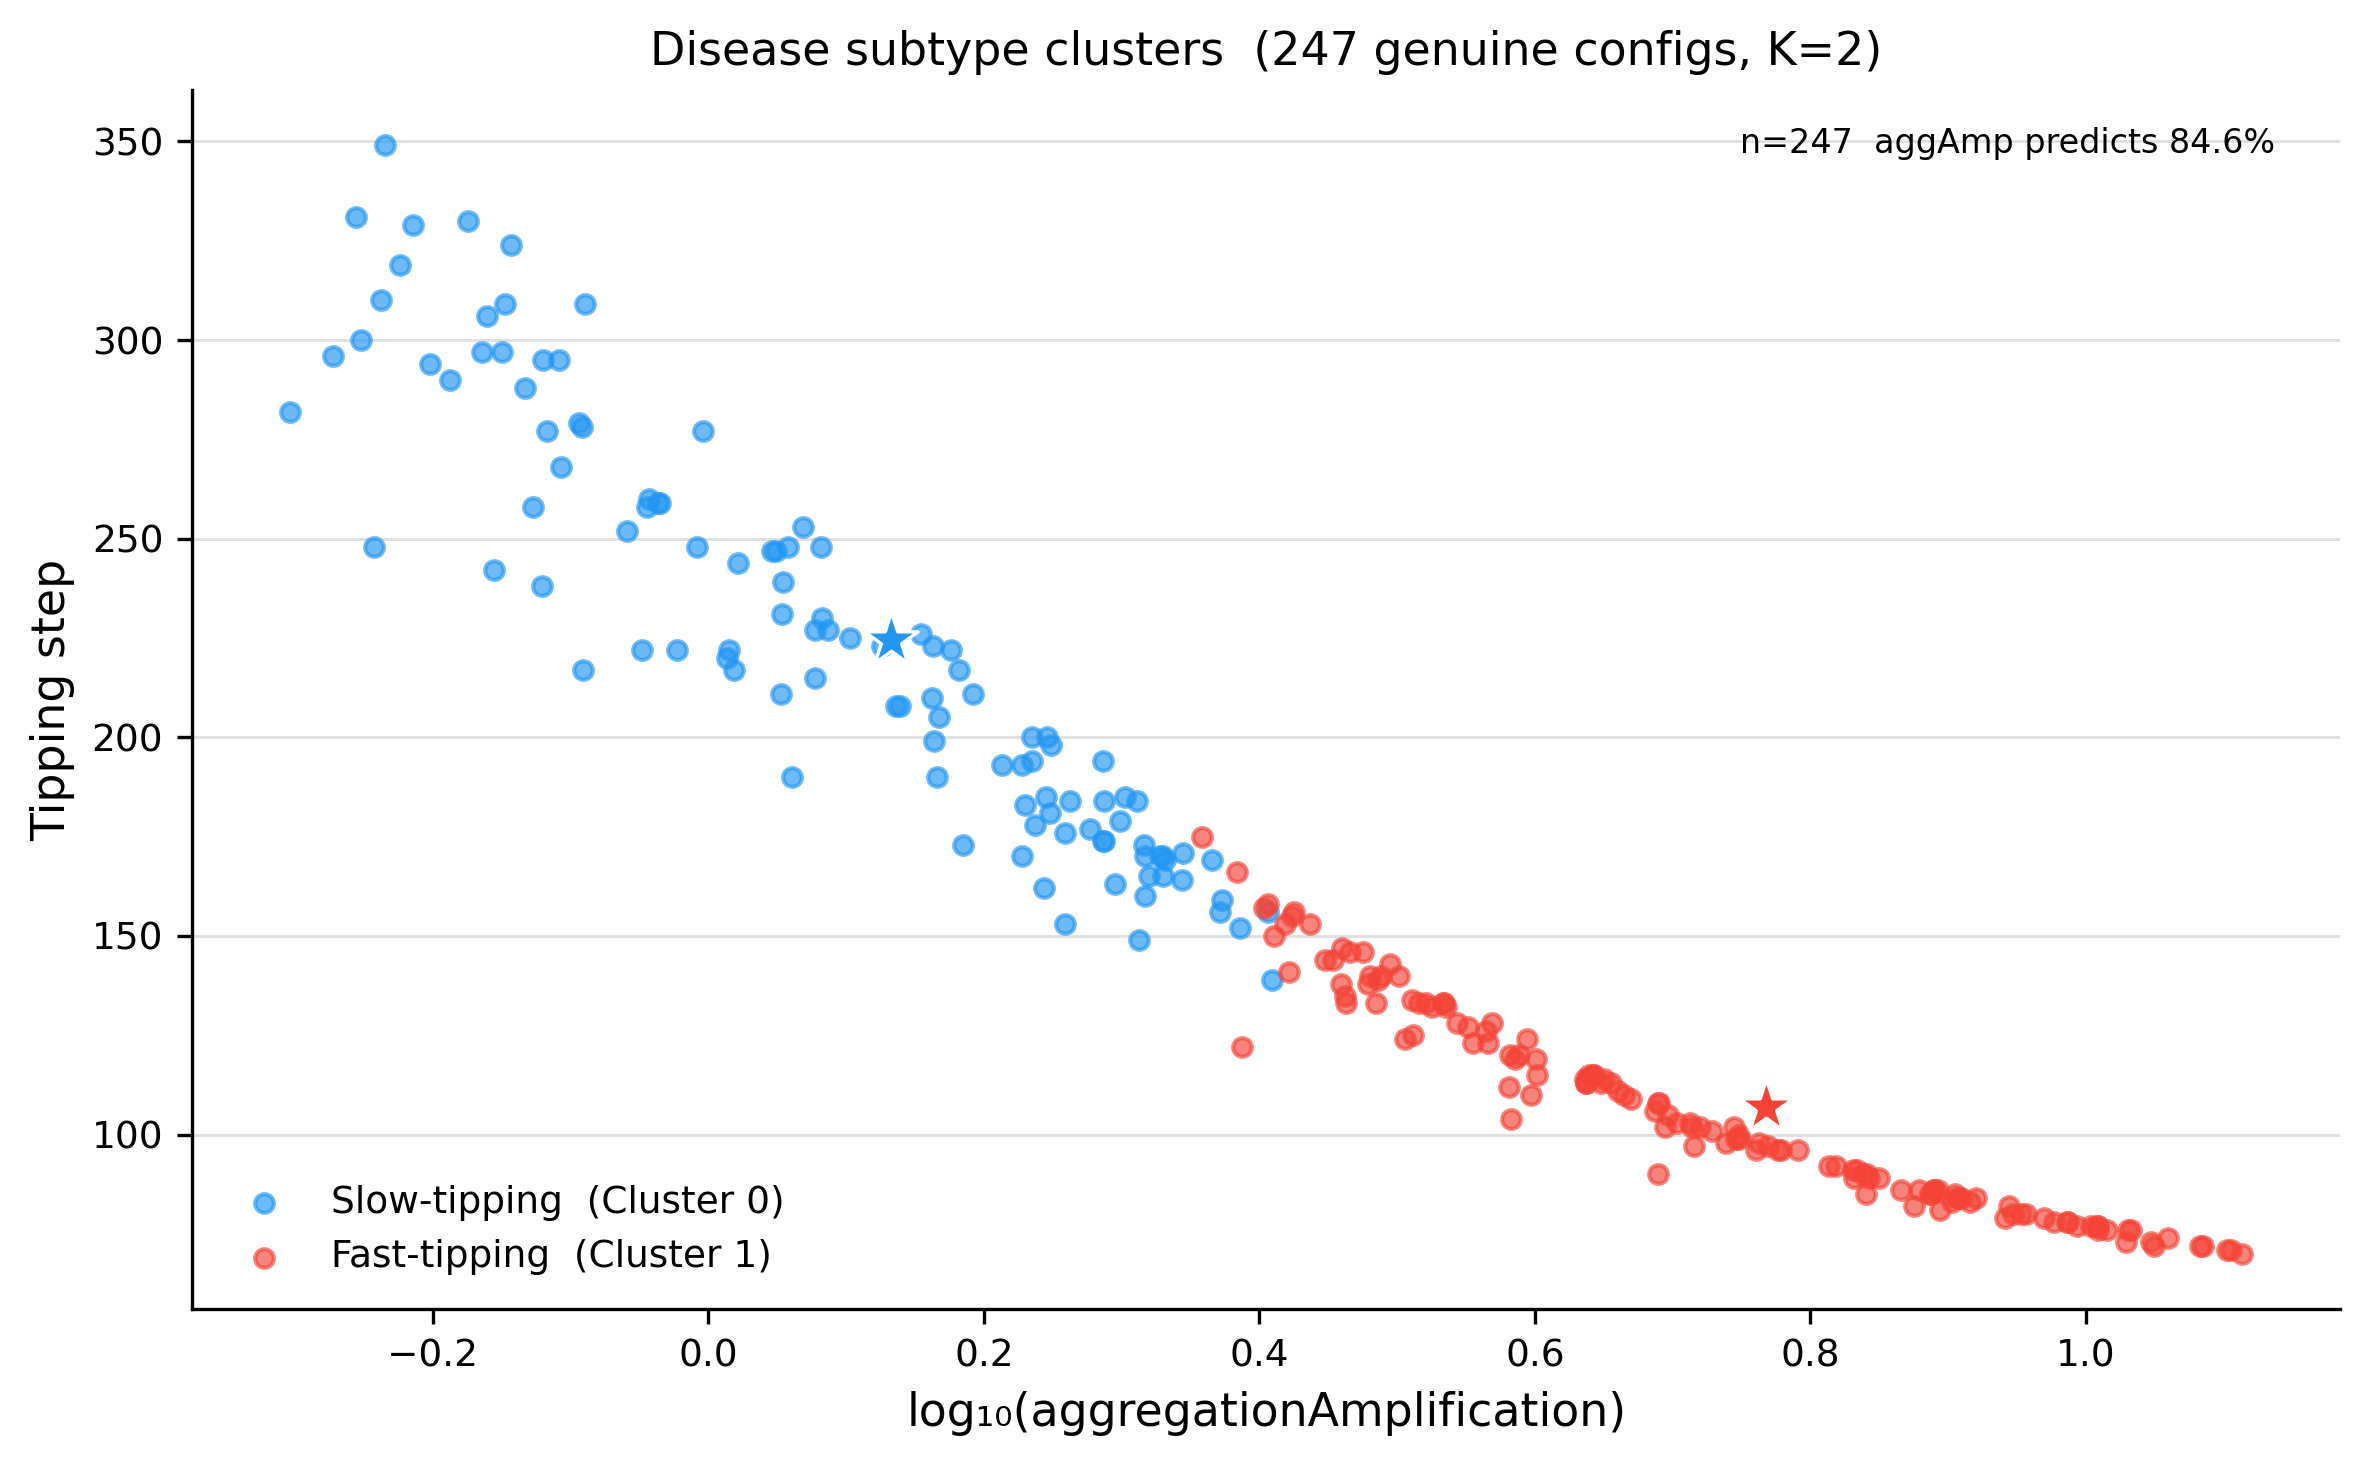
\includegraphics[width=0.9\textwidth]{figures/fig7_subtype_scatter.png}
\caption{Disease subtype scatter plot: slow-tipping (C0, \texttt{aggAmp}~$\approx 1.36$) vs.\
fast-tipping (C1, \texttt{aggAmp}~$\approx 5.86$) configurations on the first two PCA
components.}
\label{fig:subtype_scatter}
\end{figure}

\begin{figure}[H]
\centering
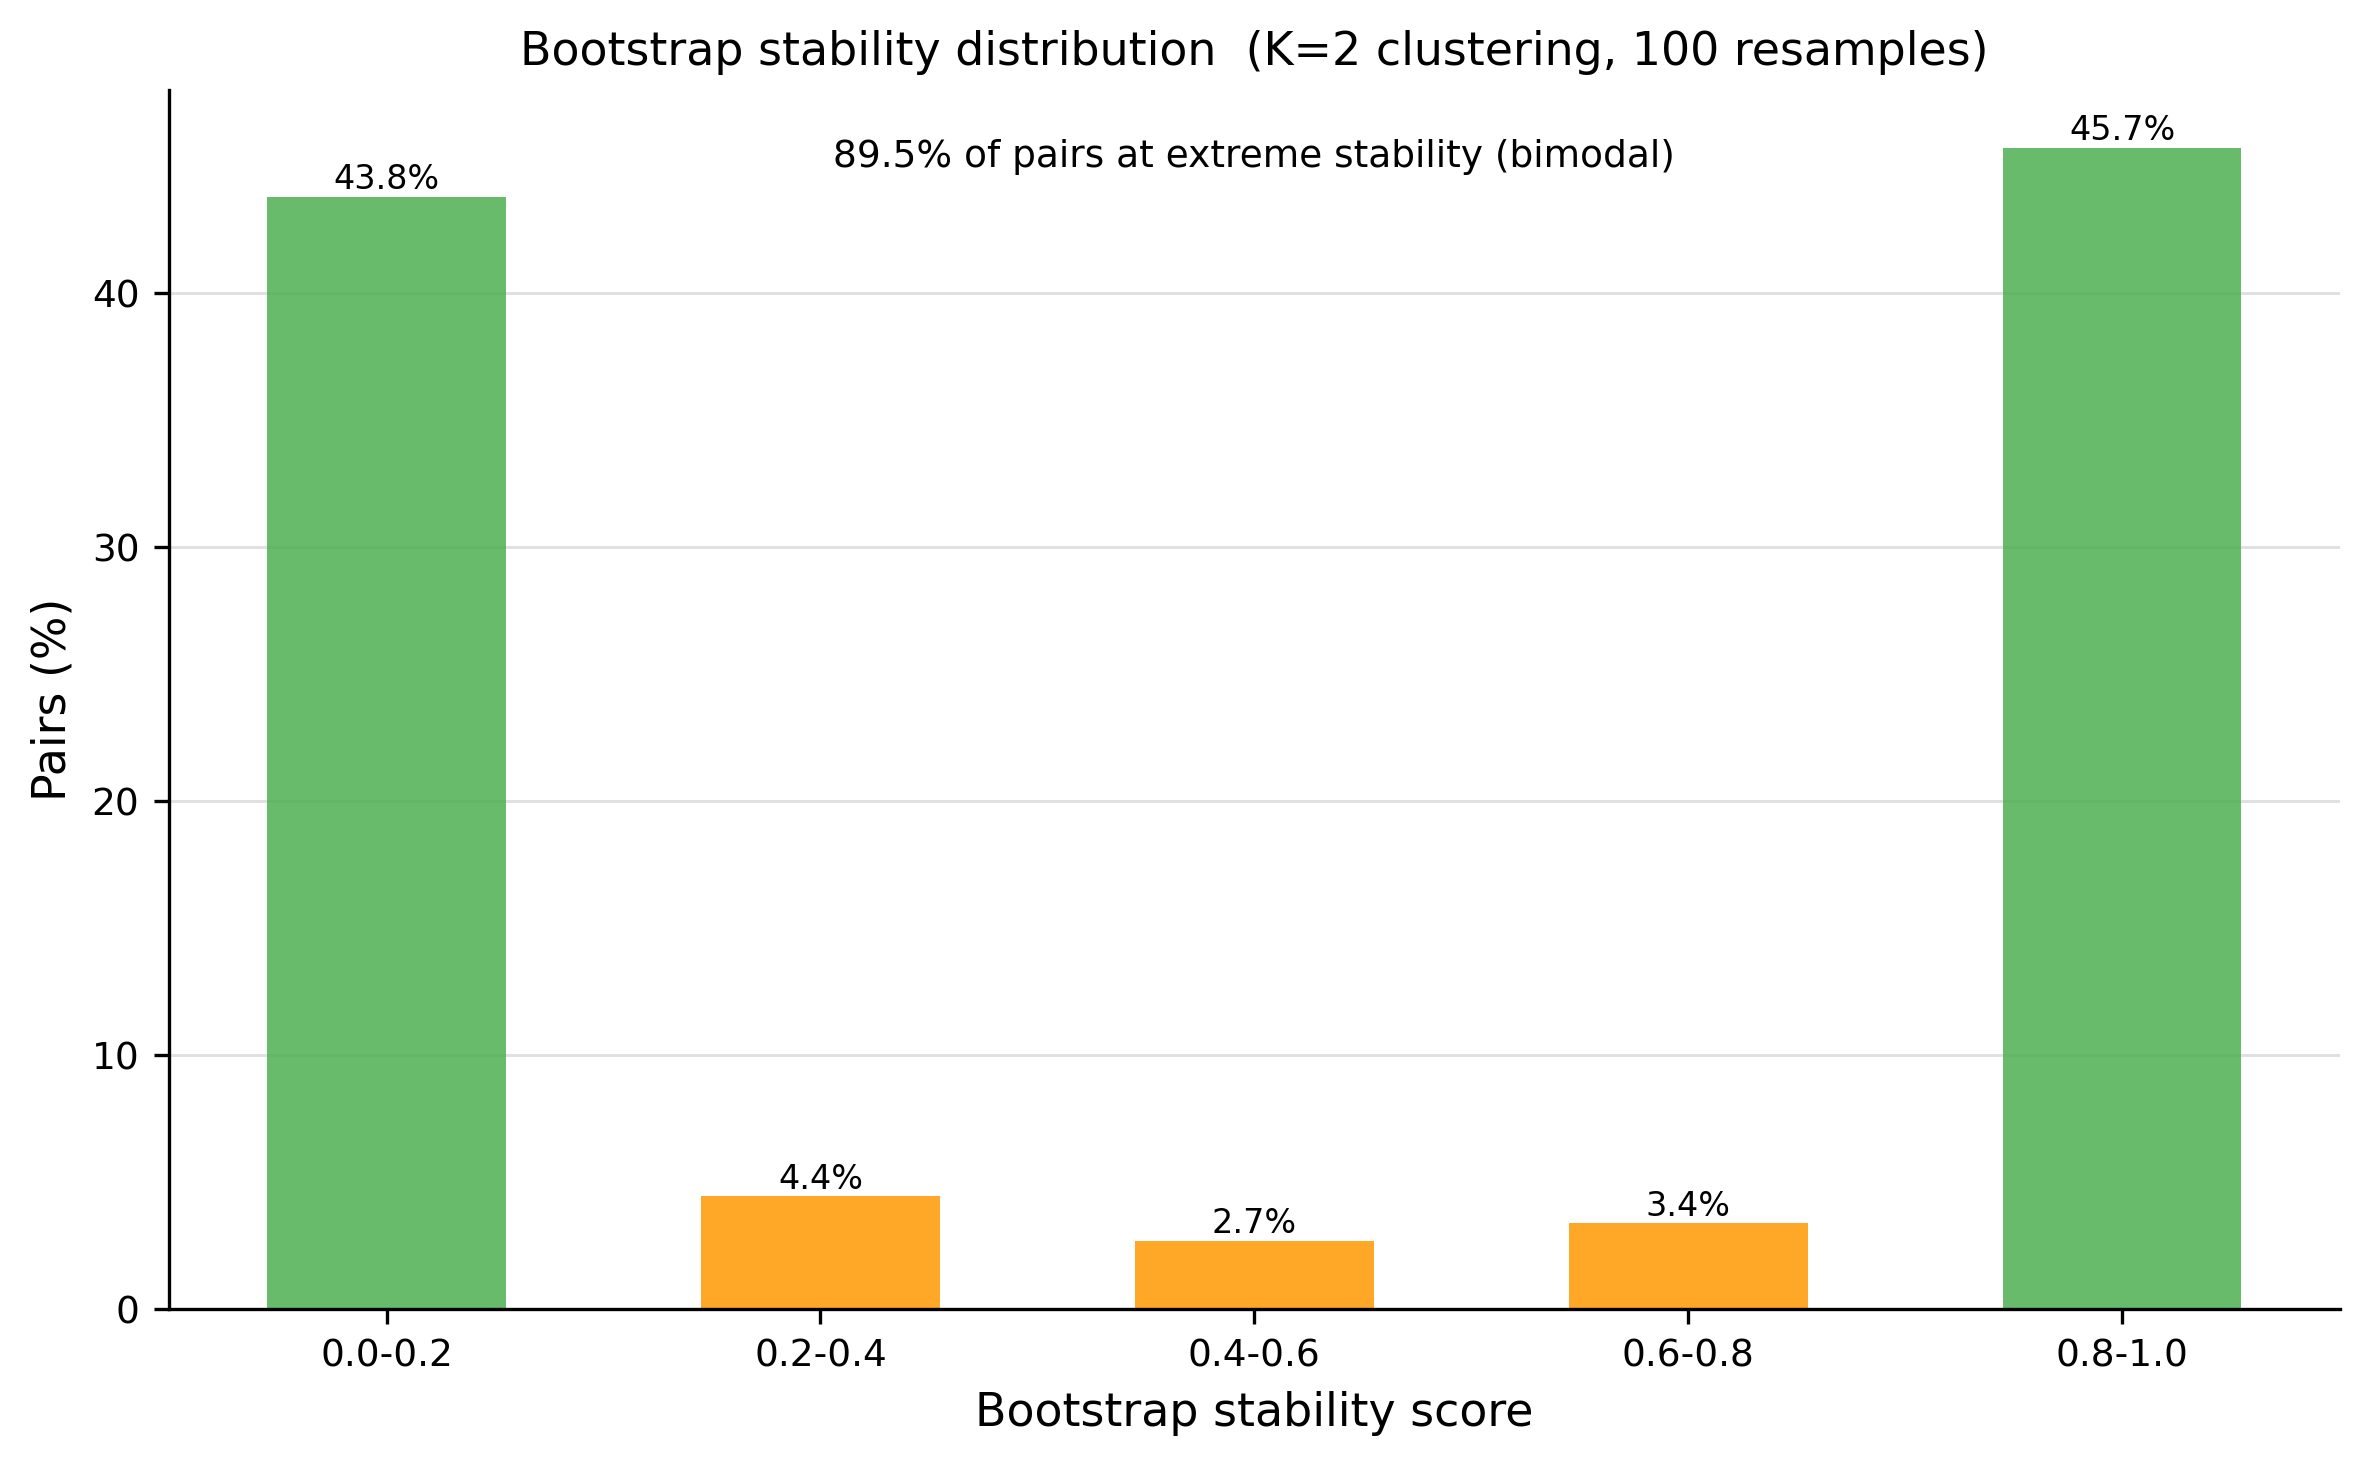
\includegraphics[width=0.9\textwidth]{figures/fig8_bootstrap_stability.png}
\caption{Bootstrap stability analysis confirming bimodal $K=2$ cluster structure. 45.7\% of
configuration pairs had stability $> 0.80$ (firmly co-clustered) and 43.8\% had stability
$< 0.20$ (firmly separated).}
\label{fig:bootstrap}
\end{figure}

\textbf{Bootstrap stability.} The $K = 2$ split showed a bimodal stability distribution across
100 bootstrap resamples (80\% of configurations each): 45.7\% of configuration pairs had
stability $> 0.80$ and 43.8\% had stability $< 0.20$, with only 10.5\% in the uncertain middle.
This bimodal pattern confirms a clean two-cluster structure despite a mean pairwise stability
of 0.51.

\textbf{Single-parameter classifier.} \texttt{aggregationAmplification} alone classified 84.6\%
of configurations correctly ($r = 0.727$) using a centroid-based threshold.
\texttt{mitochondrialFragility} was uninformative (accuracy 50.6\%, $r = -0.06$).

\subsection{Phase~13: Biological noise robustness}

All four categories of biological noise produced negligible changes in model outputs, supporting
the robustness of identified tipping points and disease subtypes across the top-10 genuine
critical configurations.

\begin{itemize}
\item \textbf{Synaptic weight noise} (up to $\pm 20\%$): Mean tipping step changed by $< 0.2\%$
relative to the unperturbed baseline; spatial coherence $r$ changed by $< 1.0\%$; genuine
tipping rate remained 1.000 at all tested levels. Verdict: \textbf{ROBUST}.
\item \textbf{Vulnerability score noise} (up to $\pm 0.20$): Tipping step changed by $< 0.6\%$;
coherence $r$ changed by $< 3.5\%$; genuine rate $= 1.000$ at all levels. Verdict:
\textbf{ROBUST}.
\item \textbf{Connectome edge dropout} (up to 10\% of synapses removed): Tipping step changed
by $< 1.9\%$; coherence $r$ changed by $< 2.1\%$; genuine rate $= 1.000$ at all levels.
Verdict: \textbf{ROBUST}.
\item \textbf{Per-neuron aggregation heterogeneity} ($\pm 20\%$): Tipping step changed by
$< 0.9\%$; coherence $r$ changed by $< 1.0\%$; genuine rate $= 1.000$. Subtype separation
fully preserved: Spearman $r = 0.976$ between baseline and perturbed tipping steps. Verdict:
\textbf{ROBUST}.
\end{itemize}

The largest observed relative change across all perturbation types and metrics was 3.5\% (coherence
$r$ under maximum vulnerability noise), well below the 10\% robustness threshold.

\subsection{Phase~14: Hierarchy of dynamical robustness}

Phase~14 sought the breaking points of each dynamical property under extreme stress (edge
dropout 30--70\%, vulnerability noise $\sigma = 0.50$--$1.00$), applied to the top-5 genuine
critical configurations over 300 simulation steps.

\textbf{Breaking points are unequal across dynamical properties.} The three tracked metrics
broke at different perturbation levels, revealing a clear hierarchy (Table~\ref{tab:breaking}).

\begin{table}[H]
\centering
\caption{Breaking points by perturbation type.}
\label{tab:breaking}
\begin{tabular}{lcc}
\toprule
\textbf{Criterion (threshold)} & \textbf{Edge dropout} & \textbf{Vulnerability noise}\\
\midrule
Genuine tipping rate $< 0.5$ & 30\% & $\sigma = 0.50$\\
Spatial coherence $r < 0.3$  & 30\% & $\sigma = 0.50$\\
Subtype rank $r < 0.5$       & \textit{not reached} & \textit{not reached}\\
\bottomrule
\end{tabular}
\end{table}

At 70\% edge dropout, the largest connected component shrank to ${\sim}20$ nodes, yet the
relative ordering of configurations by tipping speed remained intact (Spearman $r = 0.900$).
At $\sigma = 1.00$ vulnerability noise --- sufficient to essentially randomise the vulnerability
landscape --- subtype rank ordering was still perfectly preserved (Spearman $r = 1.000$)
(Figure~\ref{fig:robustness}).

\begin{figure}[H]
\centering
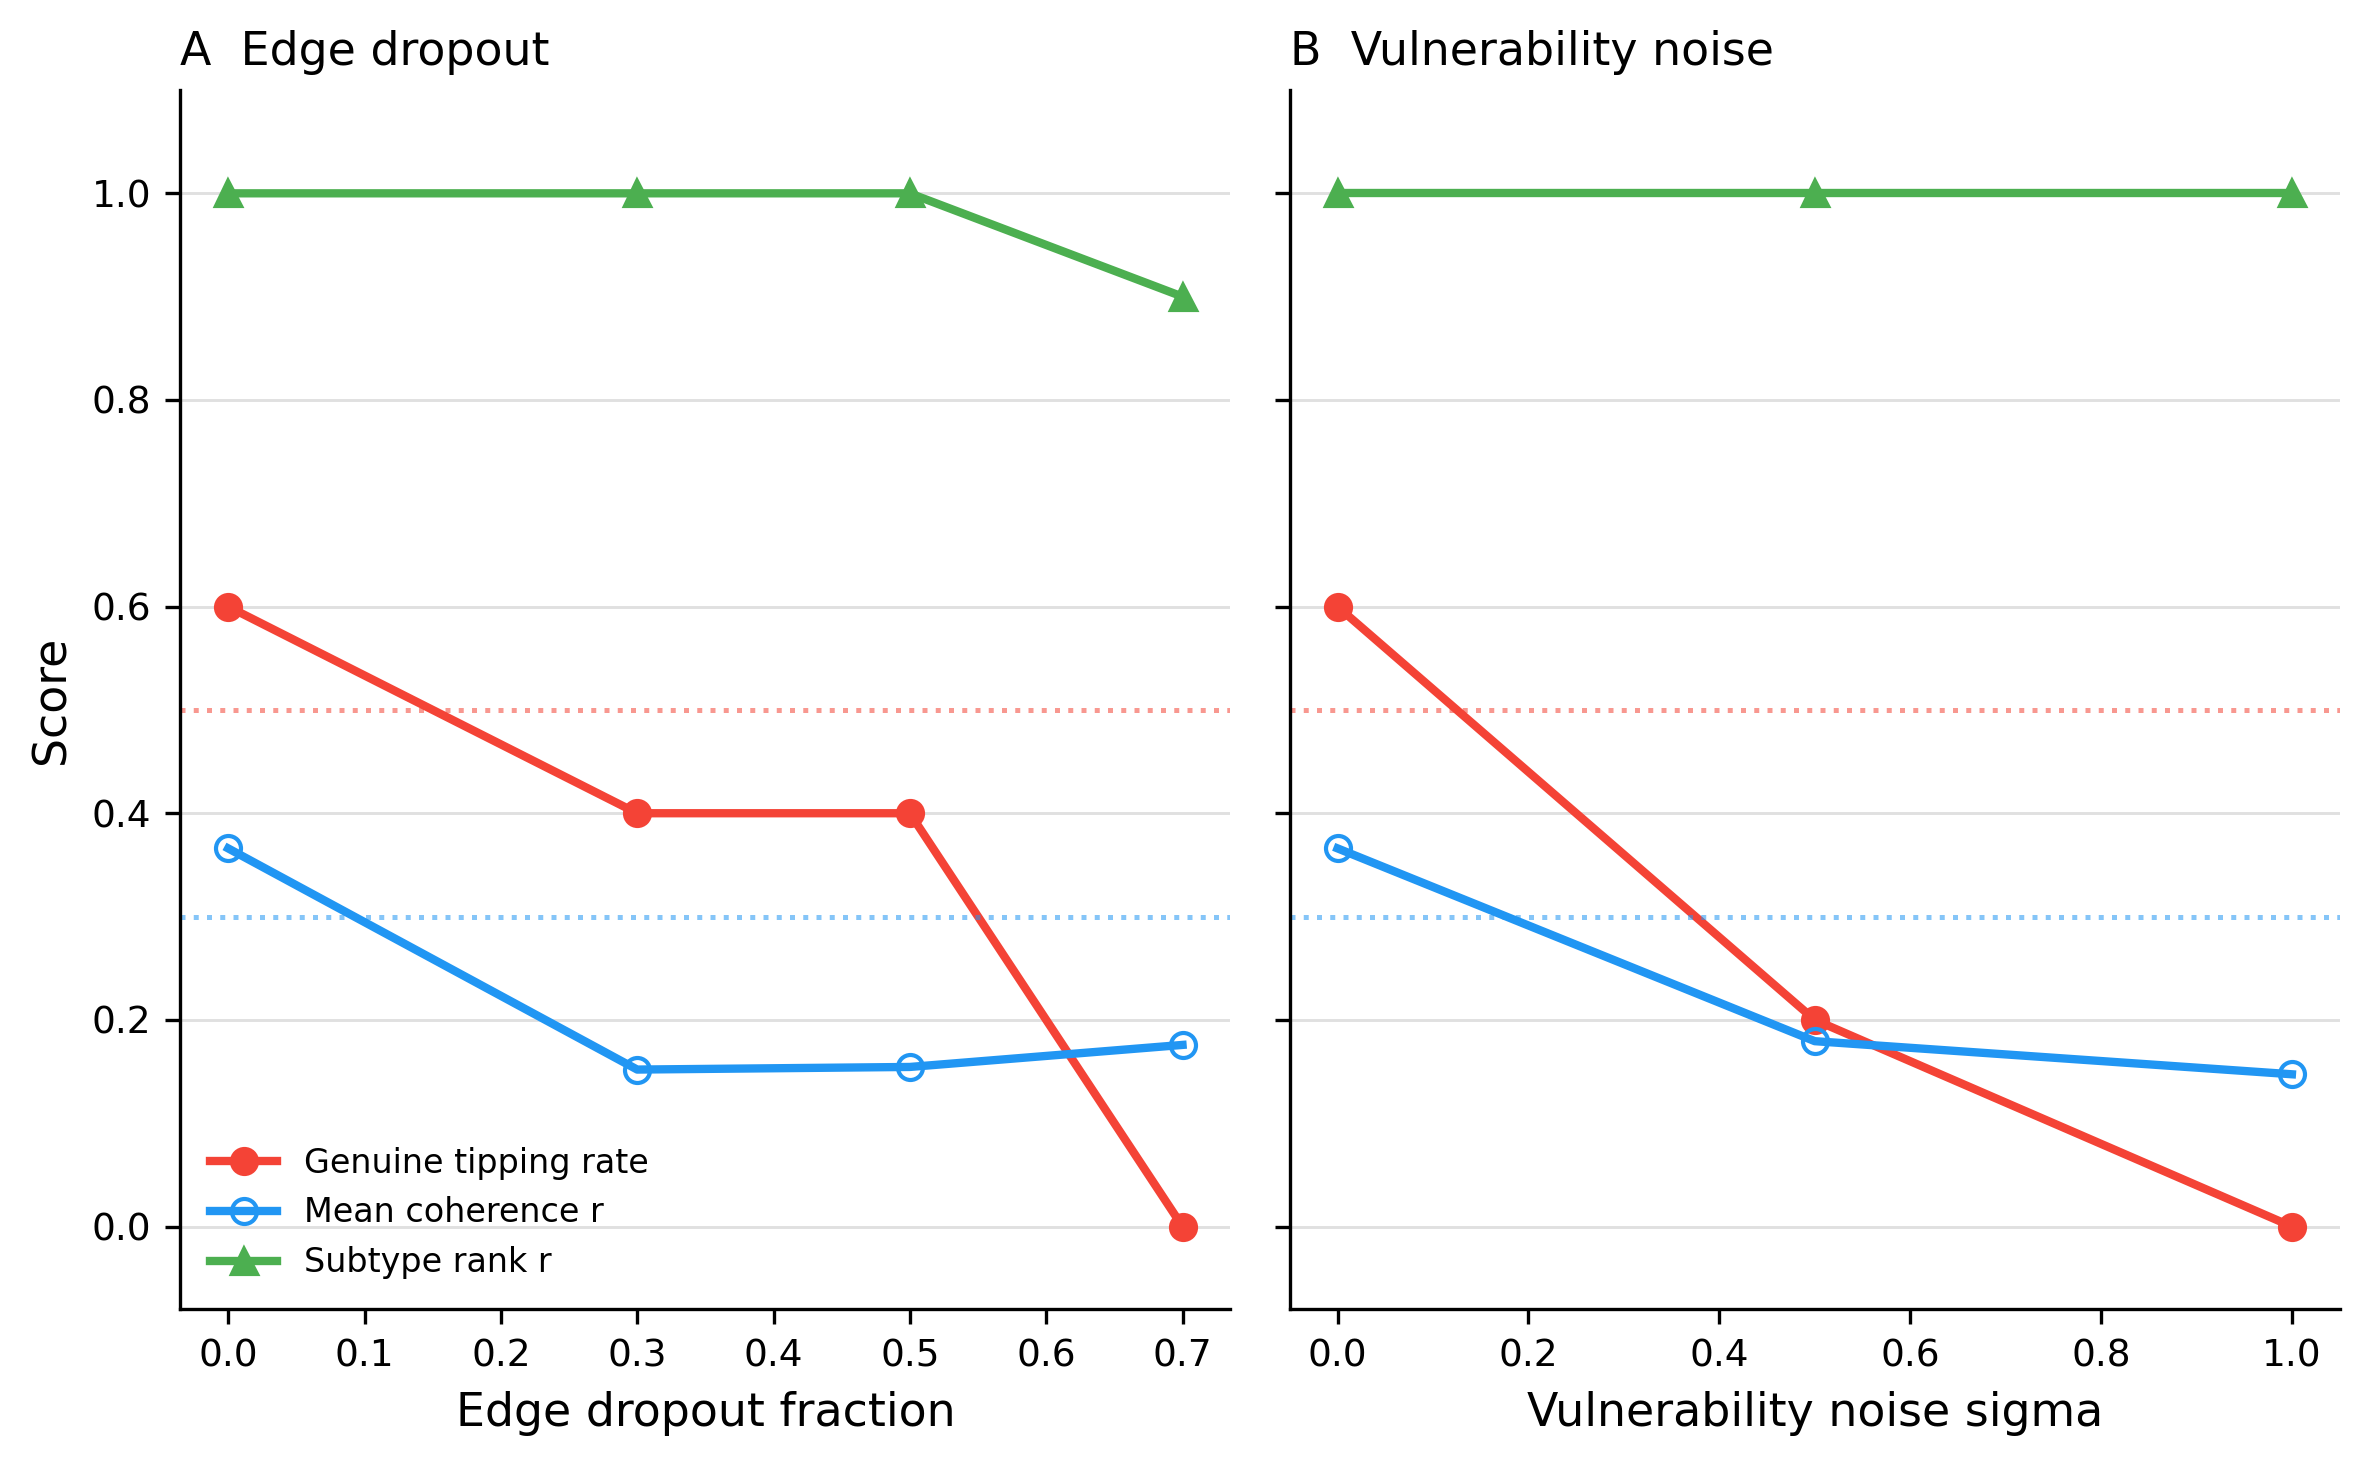
\includegraphics[width=0.9\textwidth]{figures/fig9_robustness_hierarchy.png}
\caption{Robustness hierarchy: spatial coherence and strict tipping-point structure collapse
at 30\% edge dropout and vulnerability $\sigma = 0.50$, while subtype rank ordering (Spearman
$r$) is never disrupted even at 70\% edge dropout and $\sigma = 1.00$.}
\label{fig:robustness}
\end{figure}

\textbf{Within the explored perturbation space, subtype ordering behaved as a dynamical invariant.}
Across all tested conditions, including those that completely destroyed spatial coherence and
reduced the genuine tipping rate to zero, the relative ranking of which disease configuration
degenerates fastest was never disrupted.

\subsection{Round~2 --- Topology Resilience and Pre-symptomatic Biomarkers}

Round~2 extended the core model framework to two translational questions: (1) does connectome
architecture intrinsically determine cascade resilience, and (2) can dynamical signatures
measurable before any neuron death guide therapeutic triage? Eight analysis phases (R2.1--R2.8)
were completed on all 247 genuine critical configurations from Phase~12.

\subsubsection{Motif Resilience and Efficiency Tradeoff (R2.1--R2.2)}

Nine structural topology variants of the 61-neuron motor connectome were evaluated for cascade
resilience using a composite RES score computed over 5 configurations $\times$ 10 seeds
$\times$ 500 steps (Figure~\ref{fig:motif_resilience}). Sparse-chain topology achieved the
highest resilience (RES~$= 0.815$), marginally exceeding baseline (RES~$= 0.800$). The
performance hierarchy from most to least resilient was: sparse chain (0.815), distributed
(0.803), baseline (0.800), anti-hub (0.800), modular (0.799), bypass loops (0.796),
hierarchical (0.791), rich club (0.787), and triangle-rich (0.738). Triangle-rich feedback
loops were most destabilising, reducing plateau survivors to 8.66/61 versus 12.34/61 for
baseline --- a 30\% reduction in long-term survival.

\begin{figure}[H]
\centering
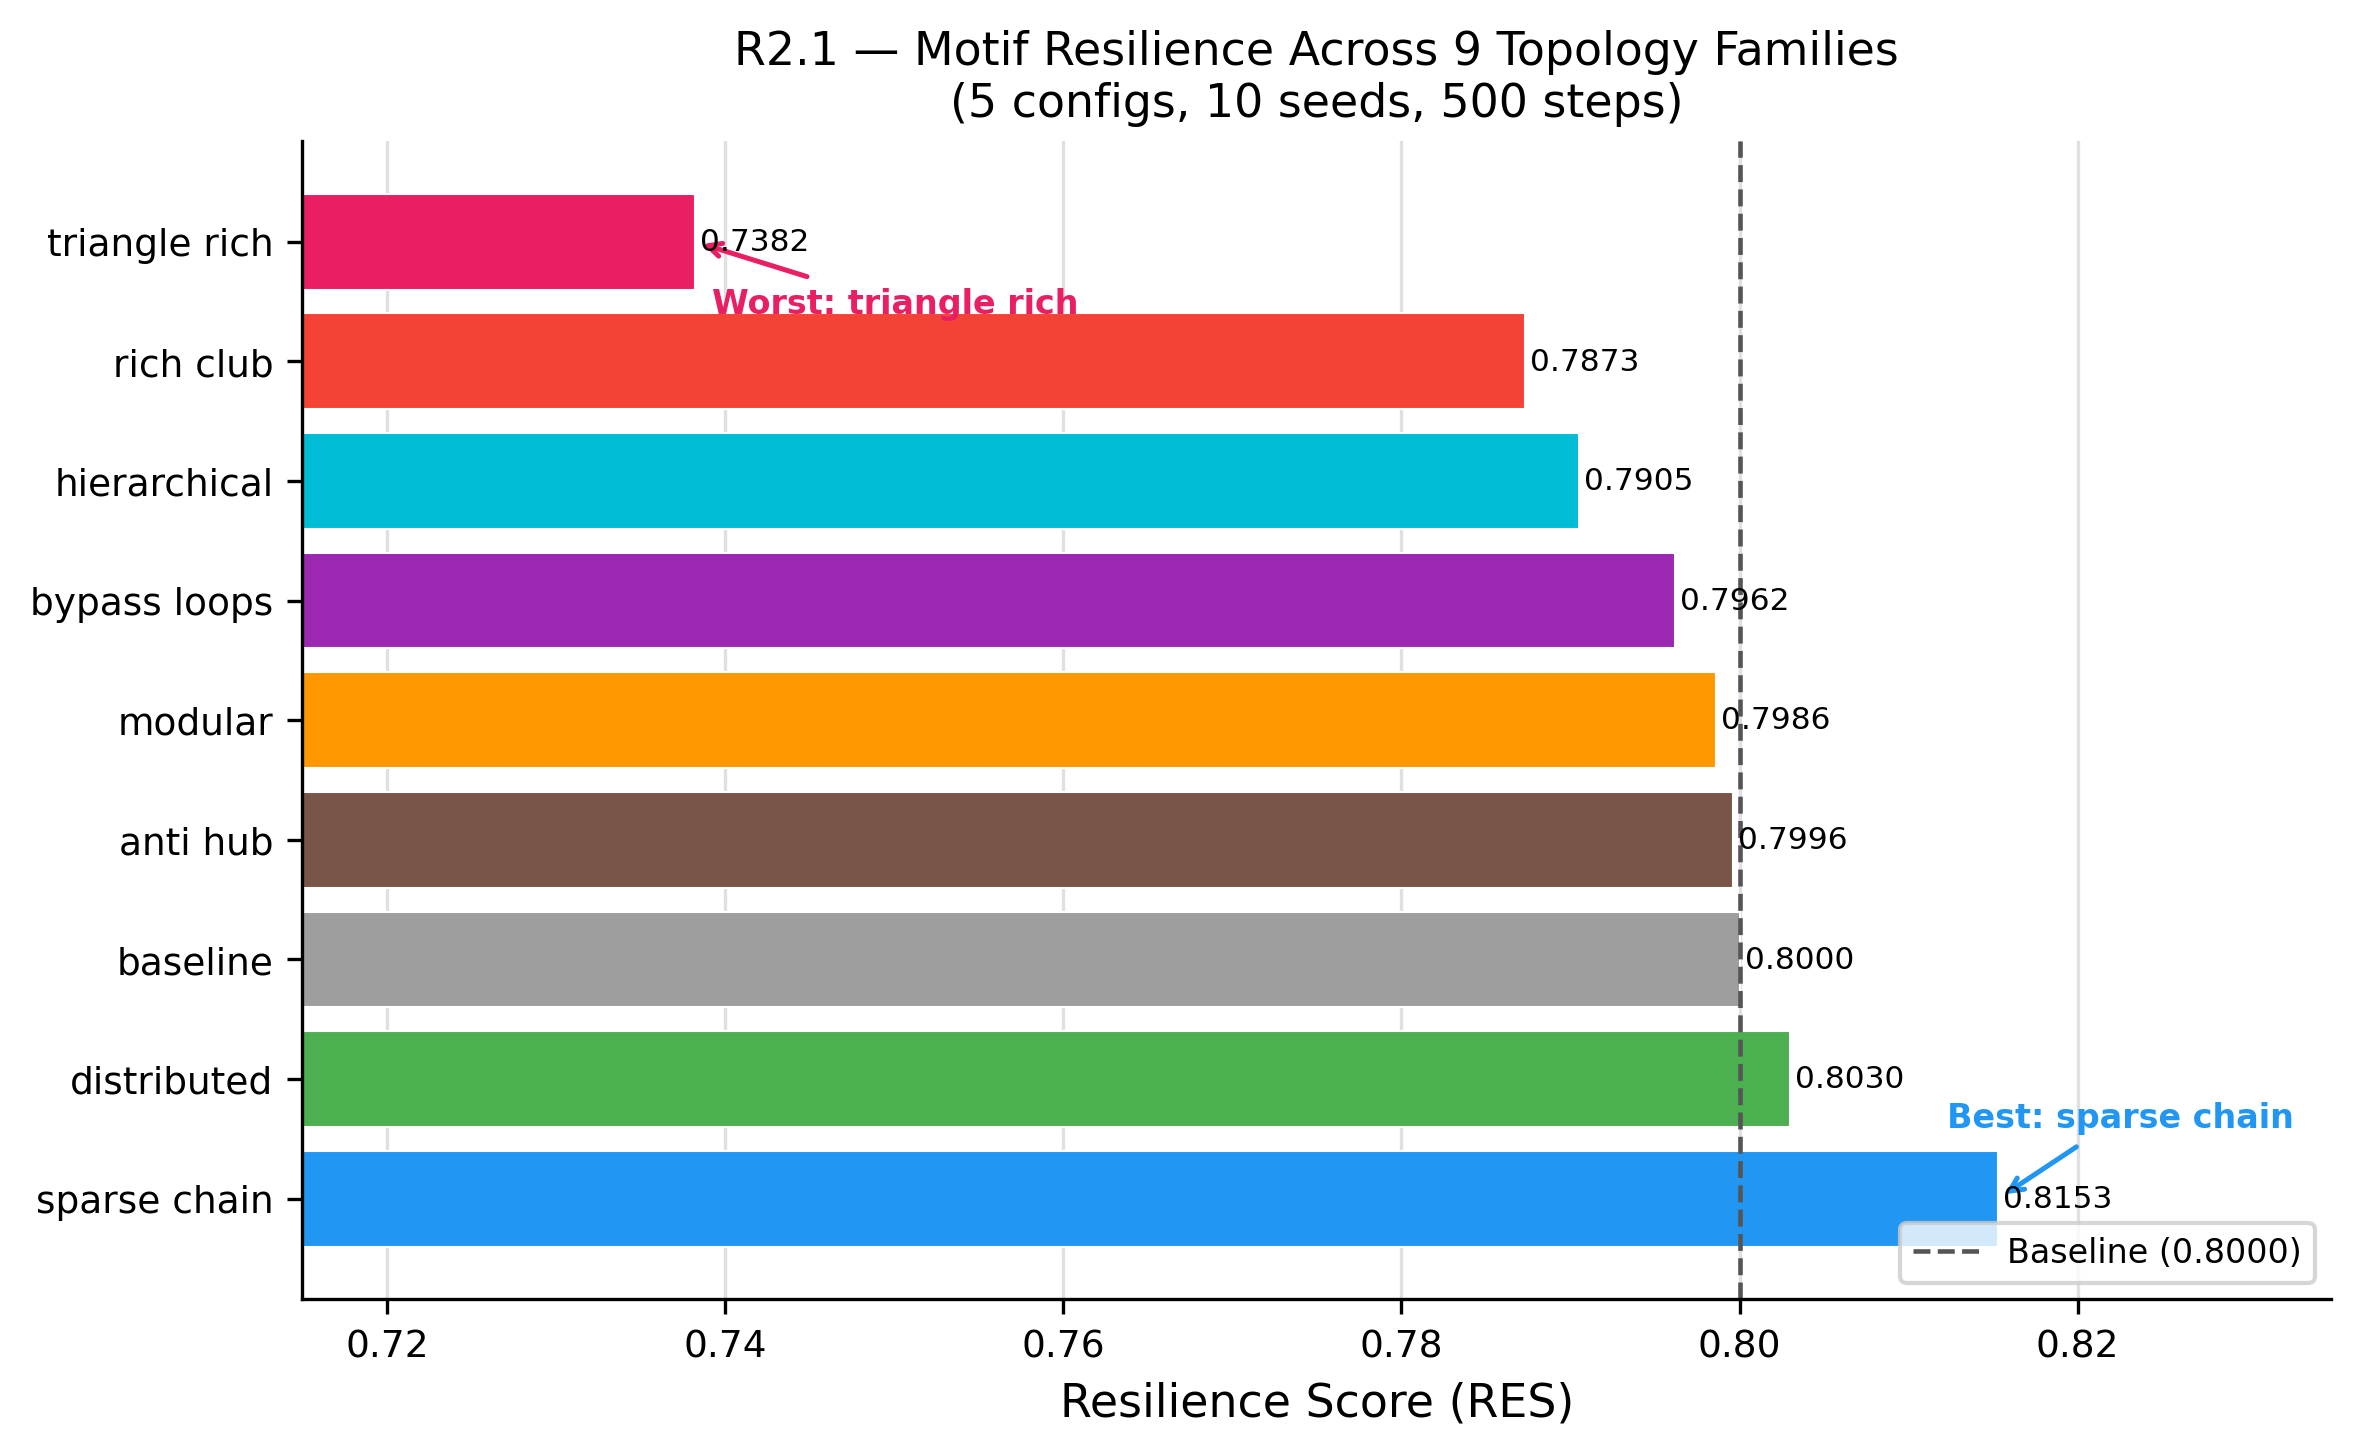
\includegraphics[width=0.9\textwidth]{figures/fig10_r2_motif_resilience.png}
\caption{Resilience scores for 9 topology variants (Round~2). Sparse-chain achieves the
highest RES~$= 0.815$; triangle-rich feedback loops are most destabilising (RES~$= 0.738$,
$-30\%$ plateau survivors vs.\ baseline).}
\label{fig:motif_resilience}
\end{figure}

The efficiency-resilience landscape was mapped across 6 topology families $\times$ 7
modification strengths (Figure~\ref{fig:efficiency_tradeoff}). A universal tradeoff was not
observed: the partial correlation between global efficiency and cascade vulnerability was only
$r = 0.439$ across all (topology, strength) combinations. Triangle-rich feedback modification
uniquely escaped the tradeoff below 60\% strength, achieving the highest Dynamical Efficiency
Index (DEI~$= 32.2$ at 60\% strength). However, above 60\% strength, the triangle-rich topology
became markedly more vulnerable. The mechanistic basis for sparse chain's resilience was
confirmed by $r(\text{tipping\_step},\, \text{global\_efficiency}) = -0.996$ within the sparse
chain series: resilience arises primarily from reduced path count, not from changes in local
clustering.

\begin{figure}[H]
\centering
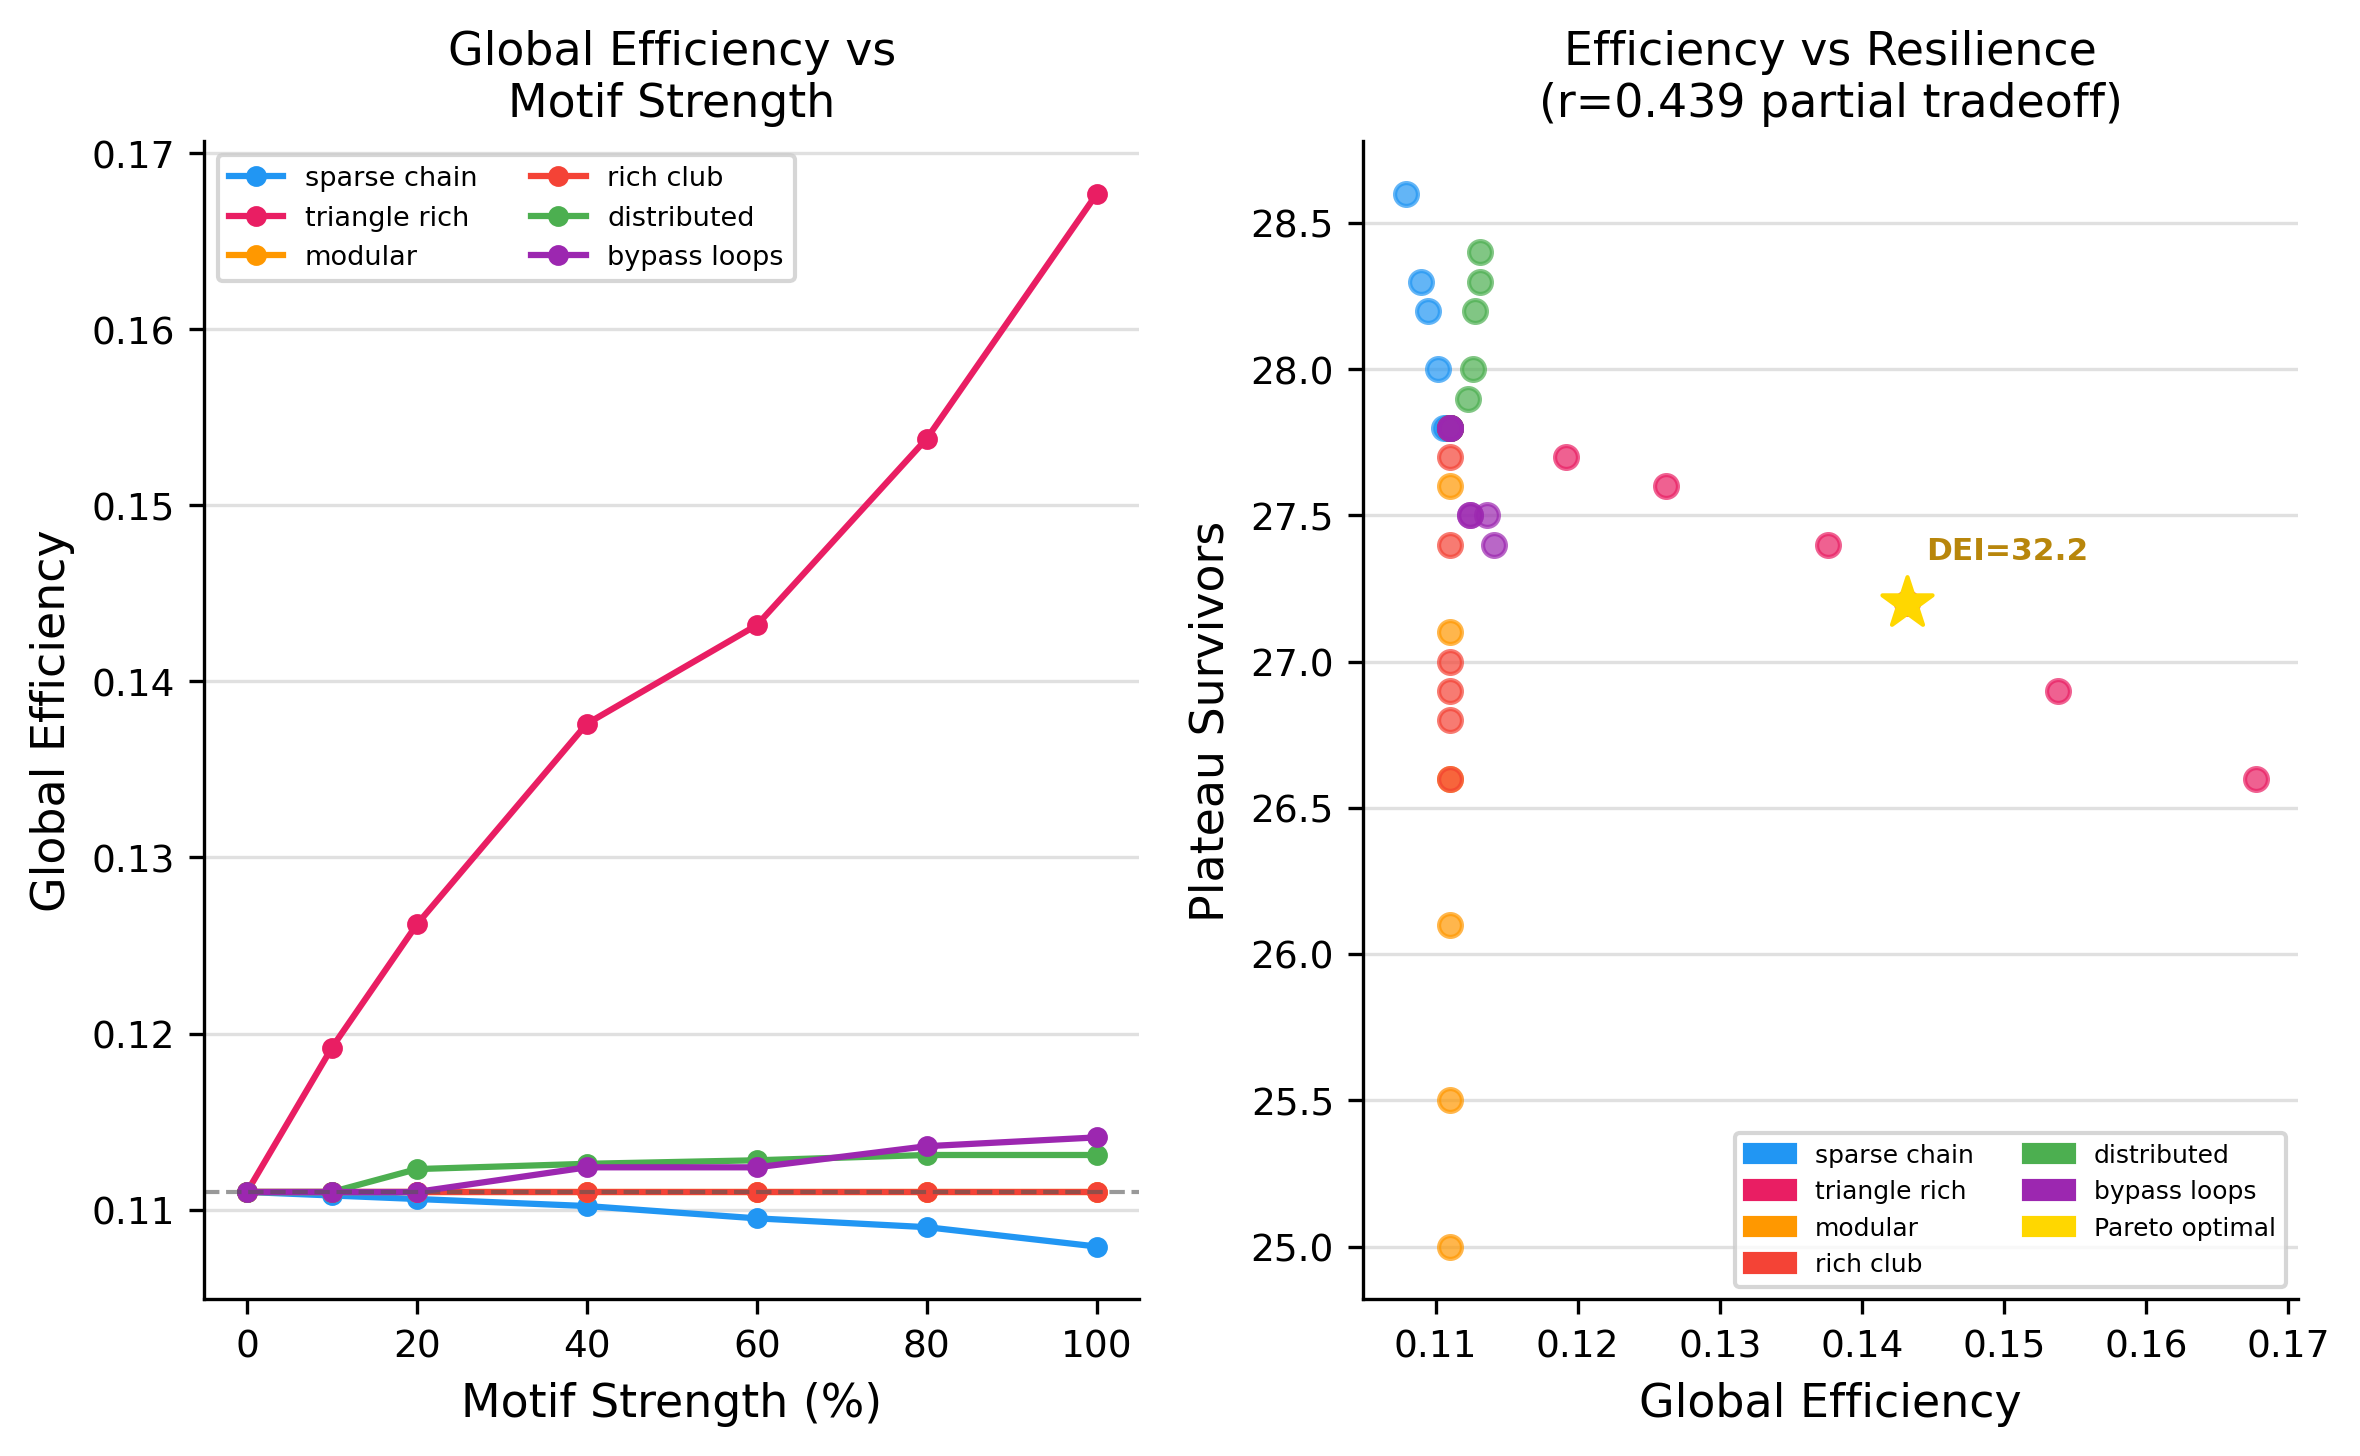
\includegraphics[width=0.9\textwidth]{figures/fig11_r2_efficiency_tradeoff.png}
\caption{Efficiency-resilience landscape across 6 topology families and 7 modification
strengths. Triangle-rich topology uniquely escapes the tradeoff below 60\% strength (DEI~$= 32.2$)
but becomes markedly vulnerable above this threshold.}
\label{fig:efficiency_tradeoff}
\end{figure}

\subsubsection{Topology-Dependent Therapeutic Boundary (R2.3)}

Whether structural modifications to the connectome could widen the therapeutic window was tested
across four topology variants using an 81-point strength $\times$ start-time grid
(Figure~\ref{fig:therapy_boundary}). The answer was unambiguously negative: all topology variants
produced identical maximum preventable start times at strength~$=0.80$ ($\mathrm{max\_start\_t}=75$ for
all variants). Fitted boundary equations are given in Table~\ref{tab:r2boundary}.

\begin{table}[H]
\centering
\caption{Therapeutic boundary parameters for four topology variants (R2.3).}
\label{tab:r2boundary}
\begin{tabular}{lcccc}
\toprule
\textbf{Topology} & \textbf{Slope} & \textbf{Intercept} & \textbf{$R^2$} & \textbf{Window area}\\
\midrule
Baseline \textit{C.~elegans} & 175 & $-62$  & 0.942 & 17\\
Sparse chain S$=100\%$       & 175 & $-62$  & 0.942 & 17\\
Triangle rich S$=60\%$       & 225 & $-102$ & 0.920 & 16\\
Triangle rich S$=100\%$      & 175 & $-72$  & 0.817 & 15\\
\bottomrule
\end{tabular}
\end{table}

\begin{figure}[H]
\centering
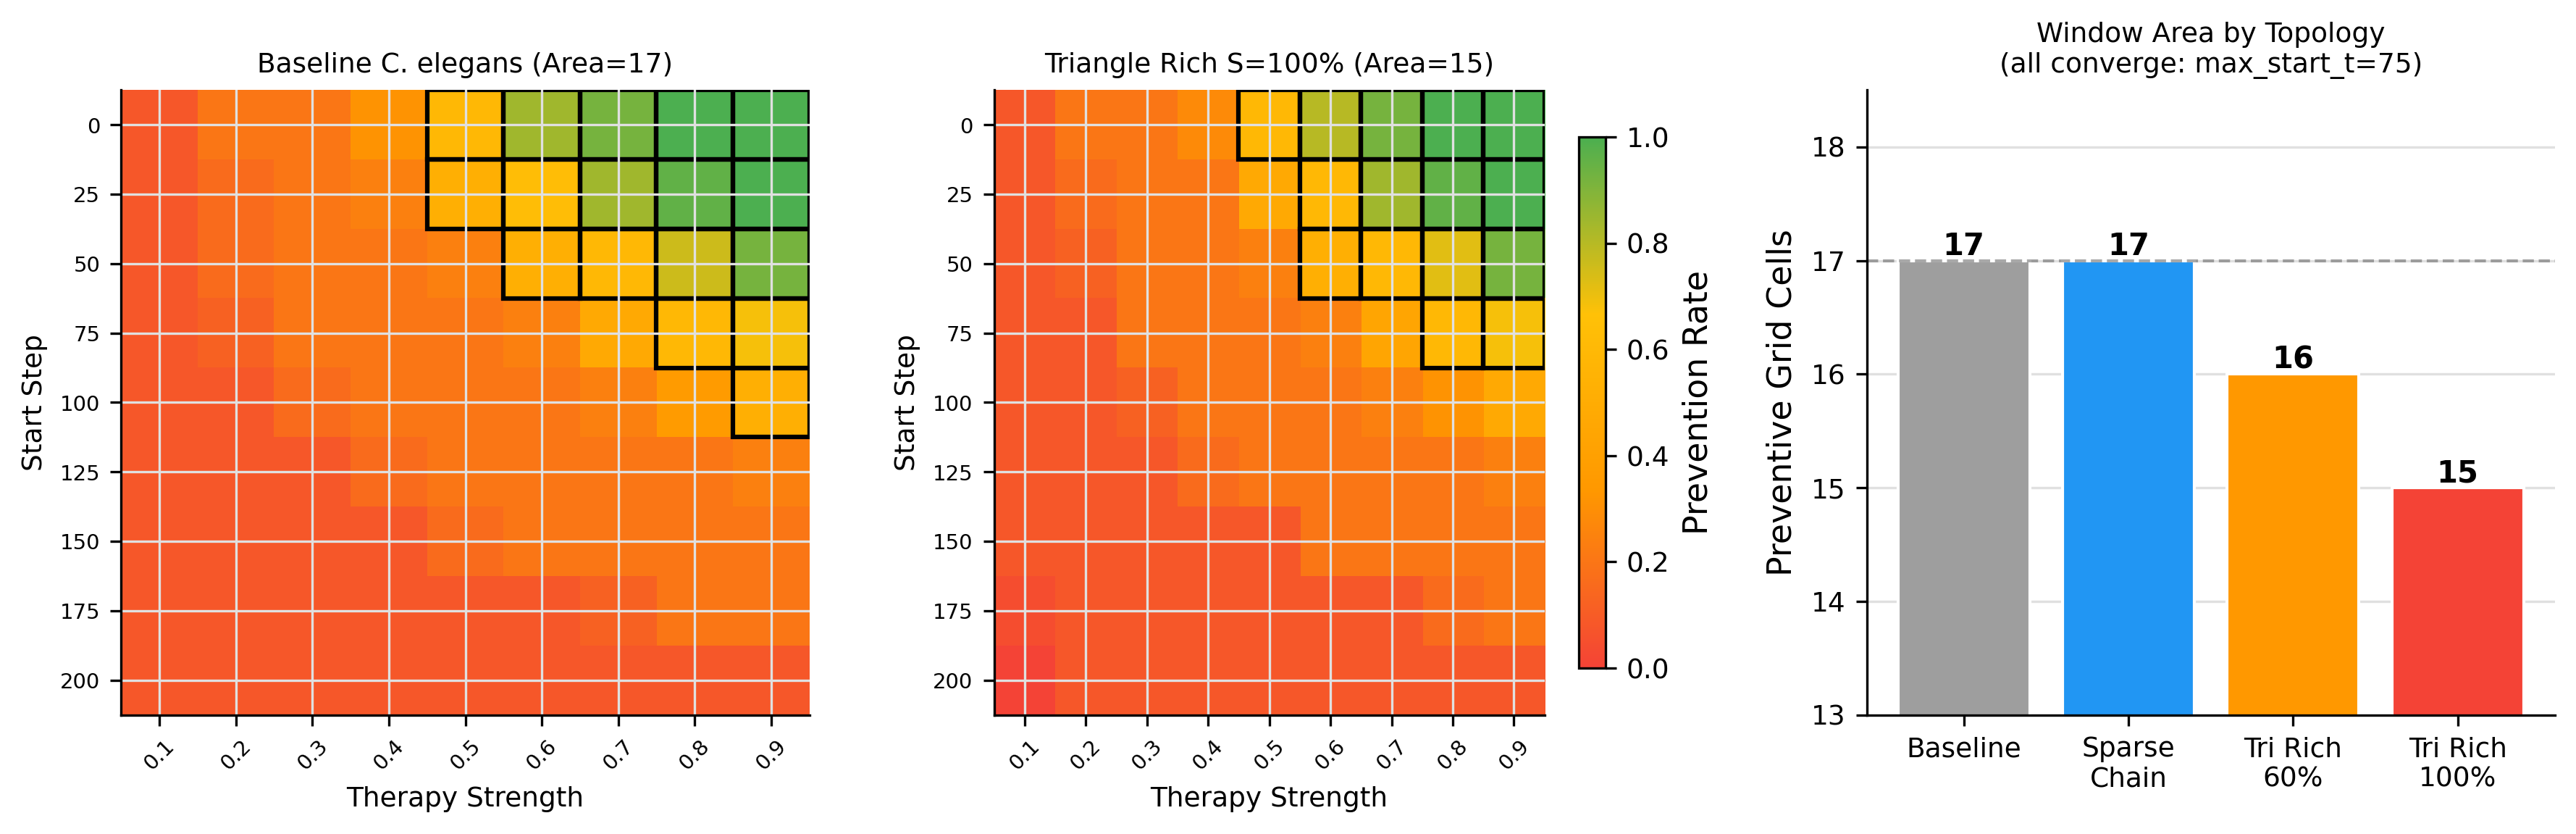
\includegraphics[width=0.9\textwidth]{figures/fig12_r2_therapy_boundary.png}
\caption{Therapeutic boundary heatmaps and window area comparison for four topology variants.
All variants produce identical maximum preventable start times at strength~$=0.80$, confirming
that circuit architecture and pharmacological timing are independent intervention axes.}
\label{fig:therapy_boundary}
\end{figure}

This null result establishes that circuit architecture and drug timing are \textbf{independent
intervention axes}: topology modifications affect cascade dynamics (resilience, efficiency)
without expanding or contracting the pharmacological window. The clinical implication is that
hypothetical connectivity-modifying interventions would not substitute for earlier
pharmacological intervention.

\subsubsection{Subtype $\times$ Topology Interaction (R2.4)}

The two Phase~12 disease subtypes were found to respond asymmetrically to topology modification
(Figure~\ref{fig:subtype_topology}). The largest single interaction was in the triangle-rich
60\% condition for plateau survivors: C0 delta~$= -0.84$ neurons, C1 delta~$= -3.00$ neurons
(interaction~$= +2.16$), meaning fast-tipping C1 disease was harmed 3.6$\times$ more by
recurrent feedback loops than slow-tipping C0 disease. The mechanism is interpretable:
fast-tipping configs have nearly no pre-symptomatic window (tipping step~$\approx 97$), so
added recurrent loops accelerate Tier~2 cascade before any intervention can act; slow-tipping
configs (tipping step~$\approx 218$) absorb the structural change within their longer silent
phase with proportionally less damage.

\begin{figure}[H]
\centering
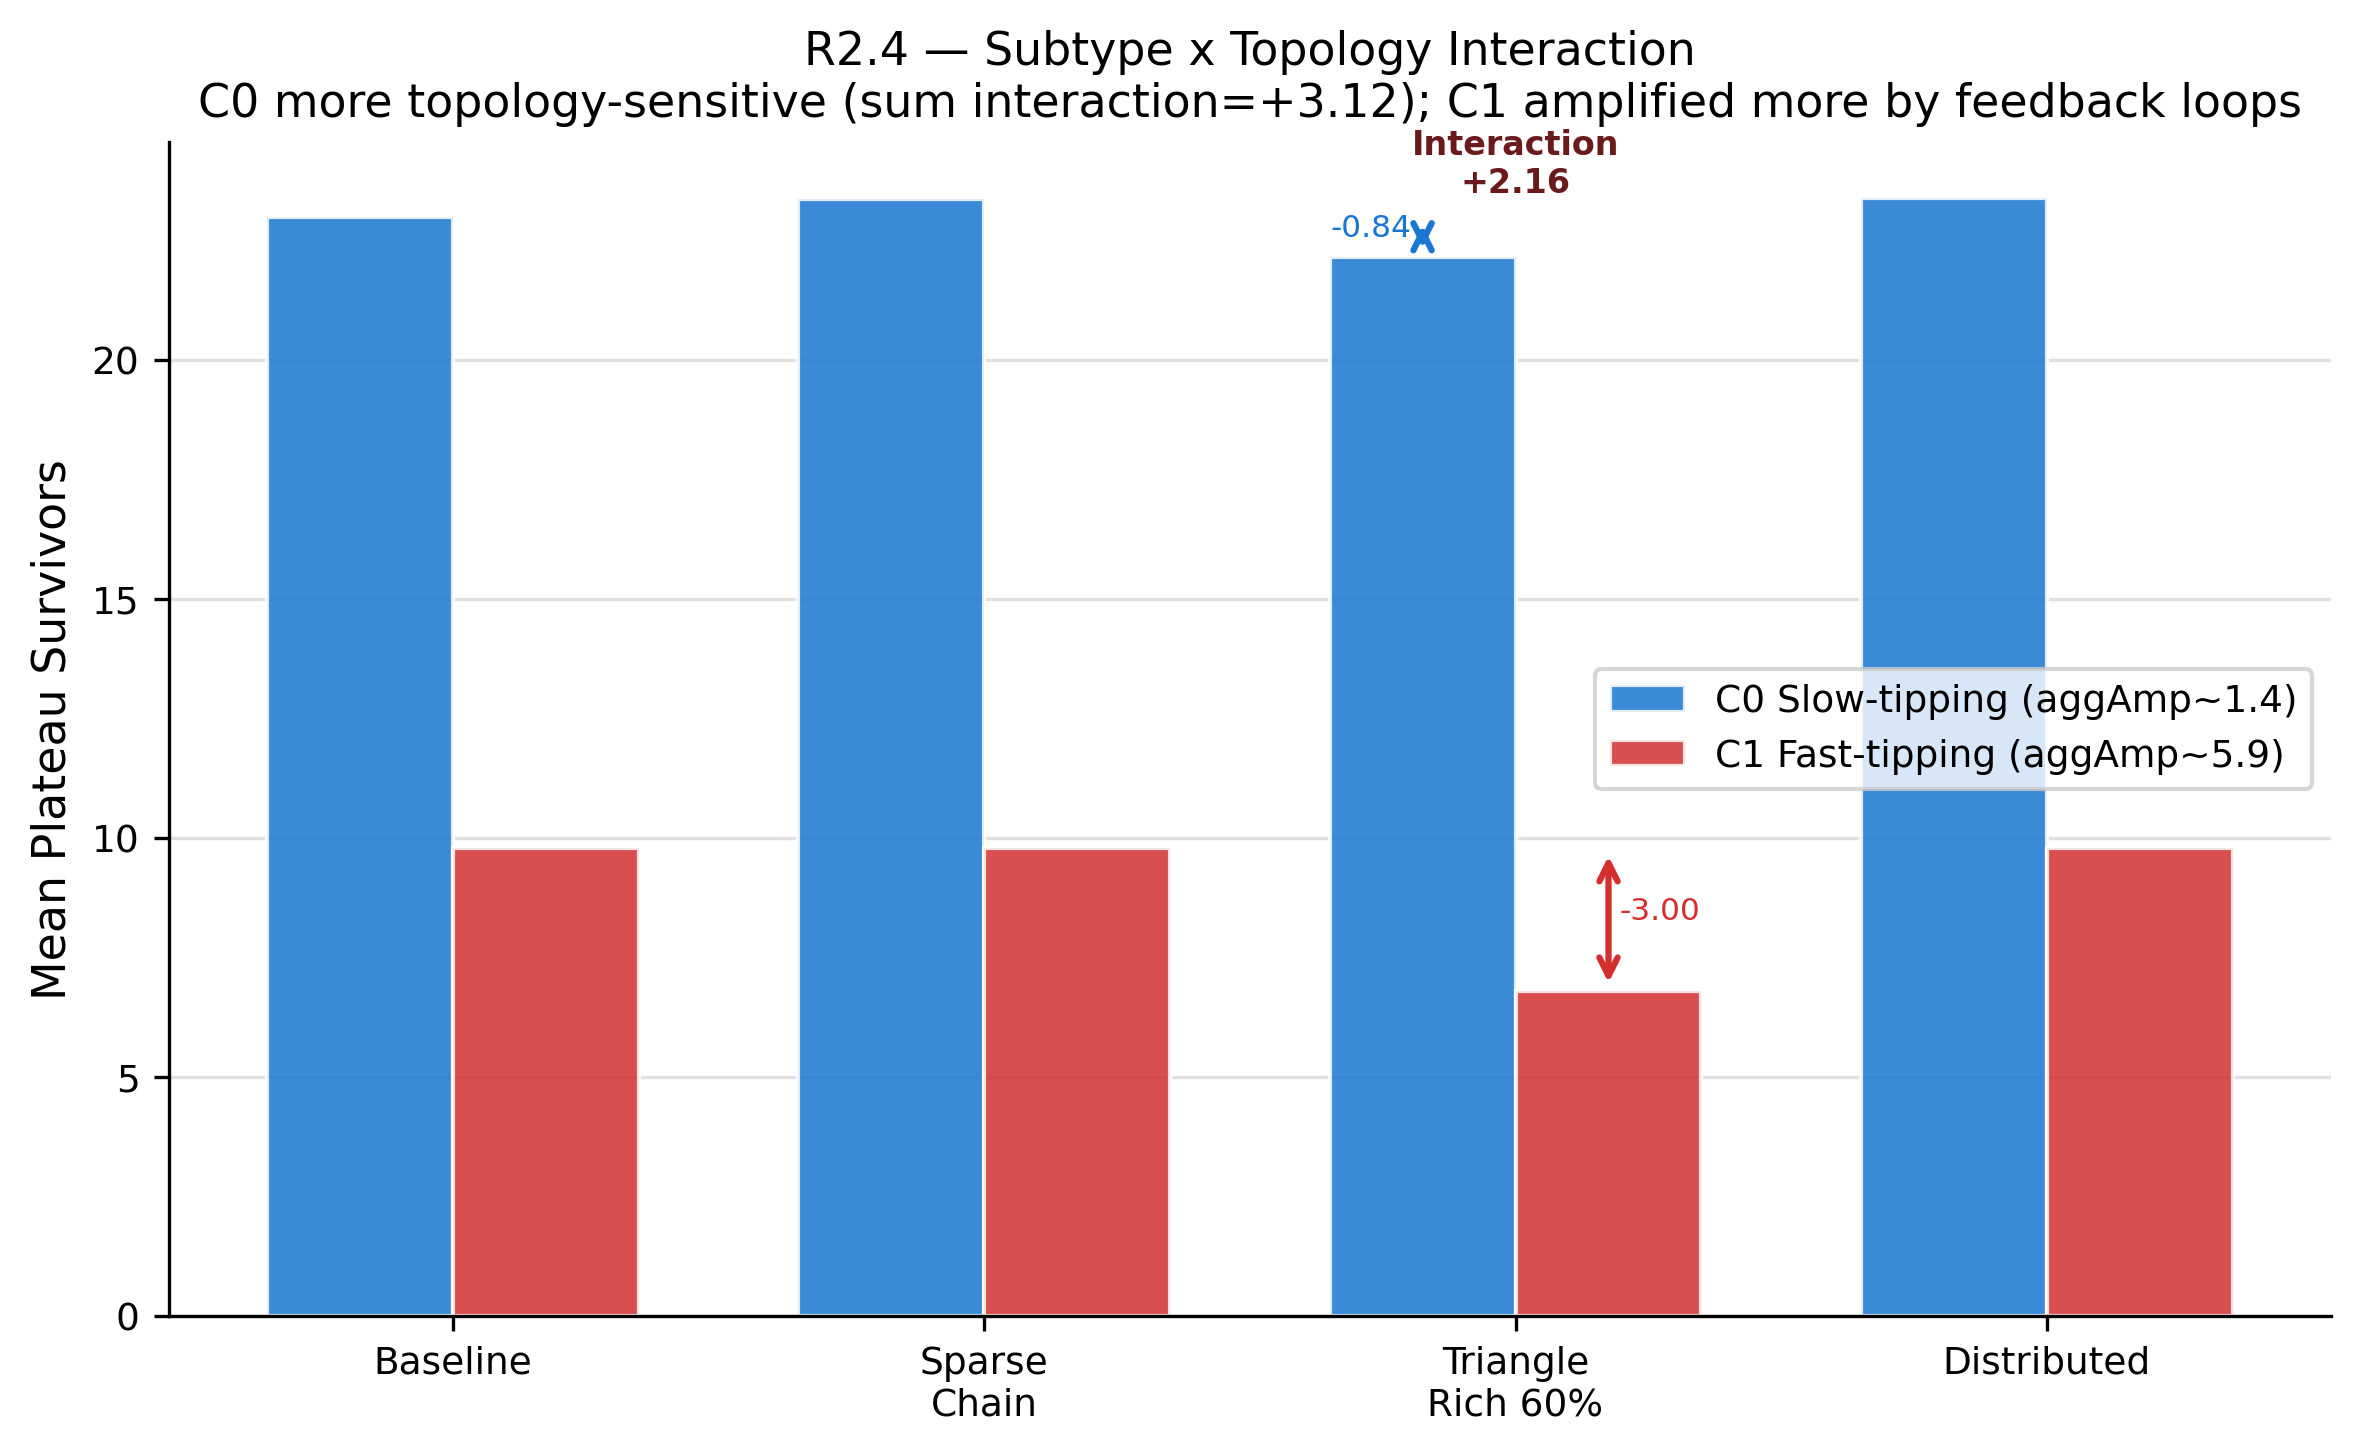
\includegraphics[width=0.9\textwidth]{figures/fig13_r2_subtype_topology.png}
\caption{Subtype $\times$ topology interaction: plateau survivors for slow-tipping (C0) and
fast-tipping (C1) disease across topology variants. Fast-tipping C1 disease is 3.6$\times$ more
harmed by recurrent feedback loops than slow-tipping C0 disease.}
\label{fig:subtype_topology}
\end{figure}

\subsubsection{Pre-symptomatic Early-Warning Signal Panel (R2.5b and R2.7)}

A central translational question was whether disease subtype and therapeutic window could be
predicted from observable dynamics at $t=50$ (before any neuron death in slow-tipping
configurations). Three pre-symptomatic features were selected from an initial panel of six
evaluated candidates and computed for all 247 configurations at $t=50$ (Figure~\ref{fig:biomarkers}):

\begin{itemize}
\item \textbf{atp\_decline\_50}: mean ATP drop across the motor circuit (ATP decline proxy,
hypothetically analogous to NfL trajectory in blood/CSF --- an unvalidated conceptual mapping).
\item \textbf{stress\_velocity\_50}: mean health decline rate per step (stress velocity proxy,
conceptually analogous to pTDP-43 phosphorylation rate --- an unvalidated conceptual mapping).
\item \textbf{agg\_slope\_50}: mean aggregation rise from baseline (aggregation slope proxy,
conceptually analogous to EMG motor nerve conduction velocity decline --- an unvalidated
conceptual mapping).
\end{itemize}

All three features showed large Cohen~$d$ for subtype separation (\texttt{atp\_decline}:
$d = 1.67$, AUROC~$= 0.860$; \texttt{stress\_velocity}: $d = 1.67$, AUROC~$= 0.999$;
\texttt{agg\_slope}: $d = 1.62$, AUROC~$= 0.999$). Ten-fold cross-validated logistic regression on all 247 configurations achieved
\textbf{88.3\% subtype classification accuracy (Phase~R2.5b, 10-fold CV on the biomarker
regression model)} at $t=50$ (std~$= 6.1\%$) --- reliably above the 80\% clinical utility
threshold --- before any motor neuron has died in slow-tipping configurations. Note that the
slightly lower figure of 87.0\% (Phase~R2.8 TWE pipeline, out-of-fold) reflects the full
end-to-end triage system rather than the isolated classifier; both are reported where relevant.
It is important to note that these features are derived from the same simulation that generates
the subtype labels --- this demonstrates internal model consistency rather than
out-of-distribution predictive validity.

\begin{figure}[H]
\centering
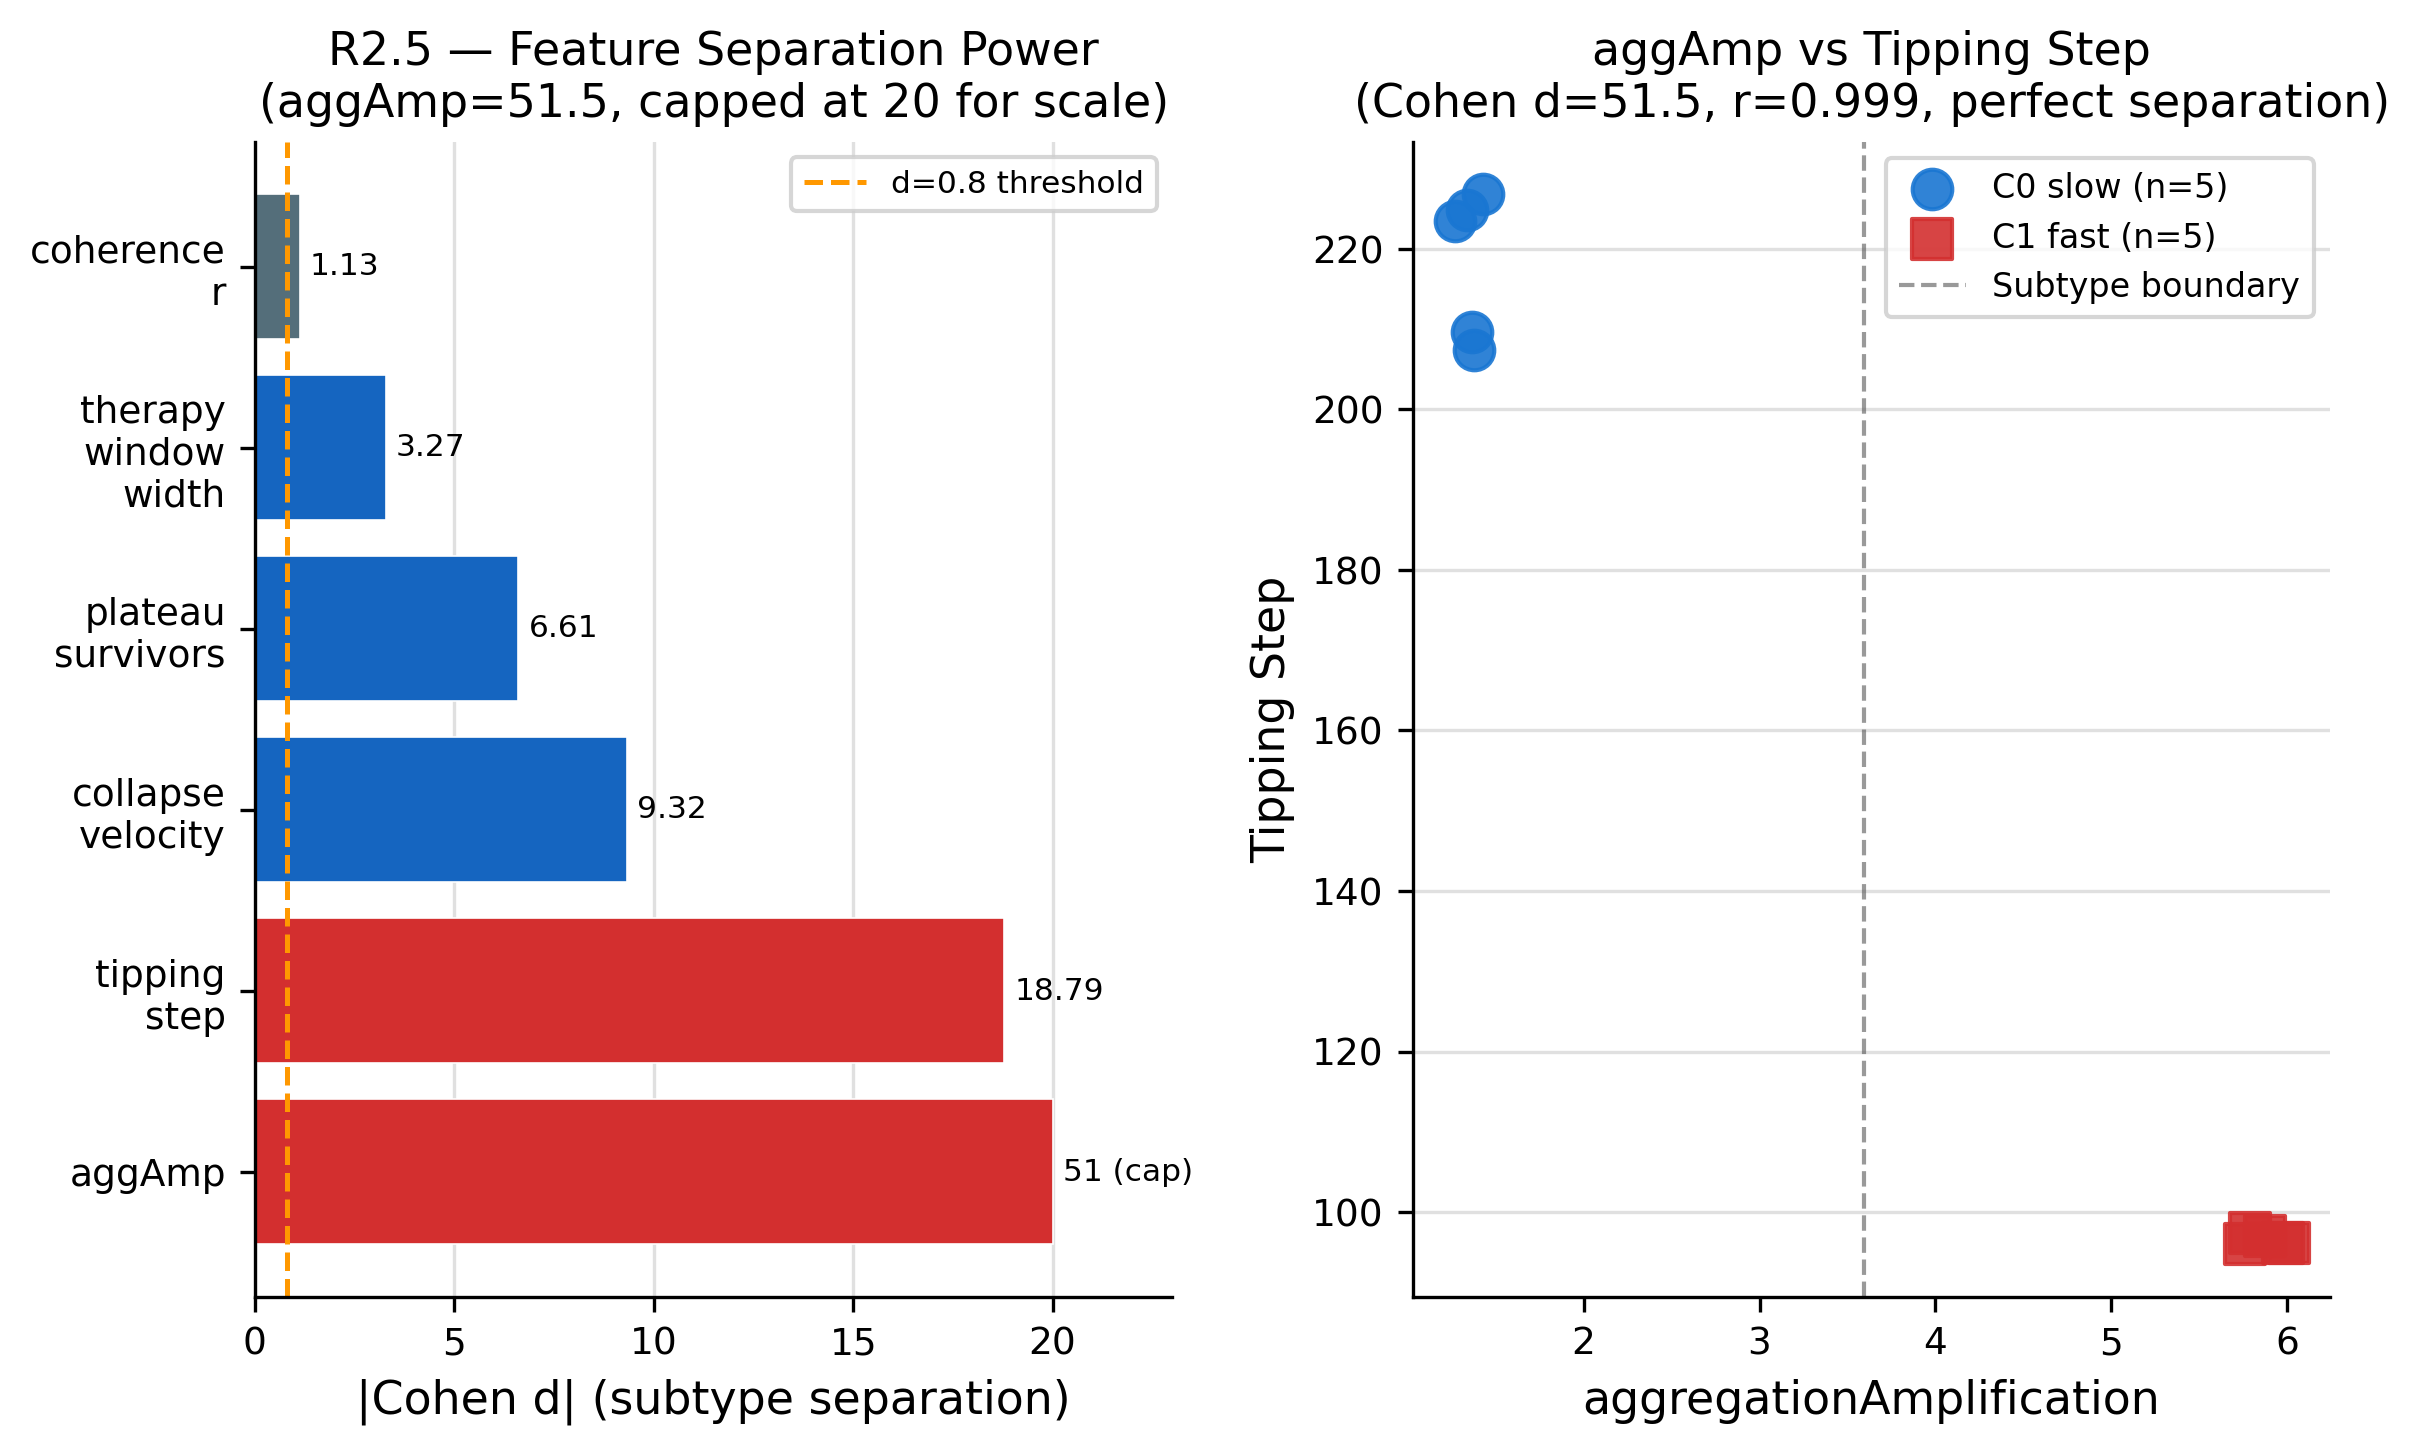
\includegraphics[width=0.9\textwidth]{figures/fig14_r2_biomarkers.png}
\caption{Pre-symptomatic simulated early-warning panel analysis. Left: Cohen~$d$ separation scores for all
6 evaluated features. Right: \texttt{aggAmp} vs.\ tipping step scatter showing complete subtype
separation. The 3-feature minimal panel (\texttt{atp\_decline\_50}, \texttt{stress\_velocity\_50},
\texttt{agg\_slope\_50}) achieves 88.3\% subtype classification accuracy at $t=50$.}
\label{fig:biomarkers}
\end{figure}

Note: an earlier analysis (Phase~R2.5b) reported $r = 0.985$ for tipping-step regression at
$t=50$ using censored tipping values (all slow-tipping configs pinned at 150 steps). This was
a censoring artifact; using uncensored Phase-7B tipping values (5 seeds, 500 steps), the true
tipping-step correlation is \textbf{$r = 0.796$}, RMSE~$= 46.1$~steps
(Phase~R2.7 regression model; Figure~\ref{fig:window_pred}).
Therapy window prediction using the same 3-feature panel achieved $r = 0.765$,
RMSE~$= 39$~steps.

\begin{figure}[H]
\centering
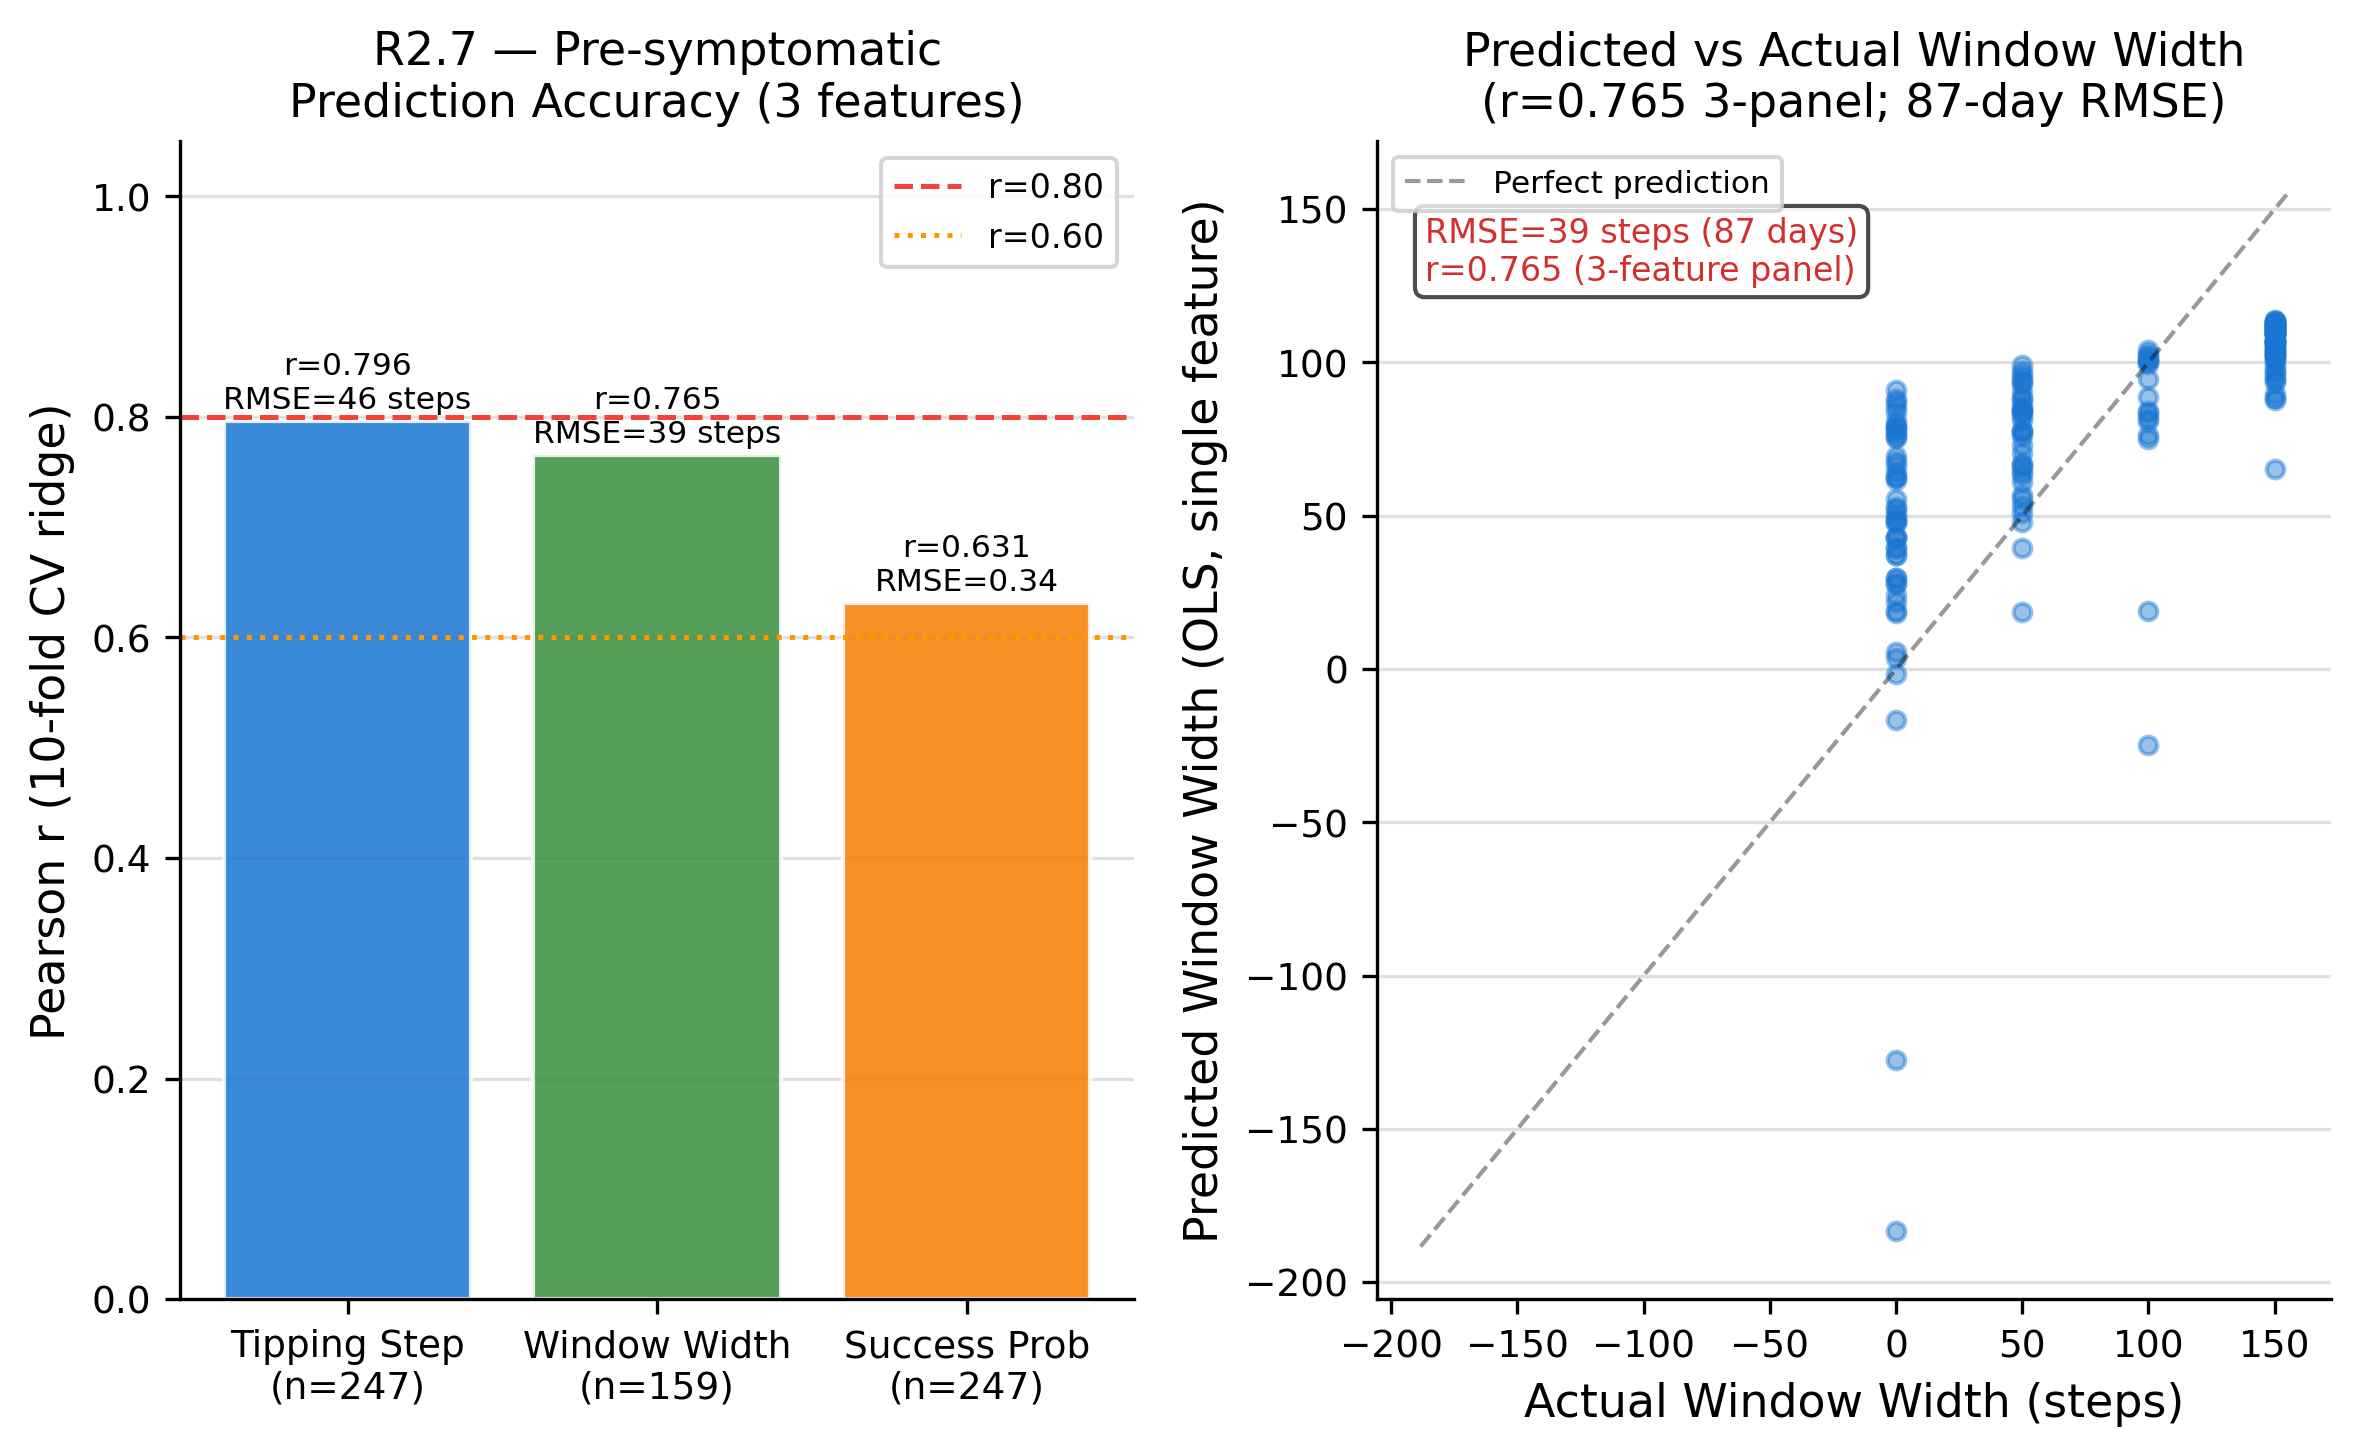
\includegraphics[width=0.9\textwidth]{figures/fig15_r2_window_prediction.png}
\caption{Pre-symptomatic prediction accuracy. Tipping-step prediction: $r = 0.796$,
RMSE~$= 46$ steps. Therapeutic window width prediction: $r = 0.765$, RMSE~$= 39$ steps. Both
using the 3-feature panel at $t=50$.}
\label{fig:window_pred}
\end{figure}

\subsubsection{Therapeutic Window Estimator (R2.8)}

The Simulated Therapeutic Window Estimator (TWE) integrates the $t=50$ biomarker predictions
into a clinical decision framework assigning each configuration to one of four intervention
strategies (Figure~\ref{fig:twe}):

\begin{itemize}
\item \textbf{Strategy~A} (Aggressive pharmacological): assigned when subtype confidence for
C1 (fast-tipping) is high ($> 0.70$); 95 configs (38.5\%).
\item \textbf{Strategy~B} (Topology-neutral therapy): assigned when therapy success probability
at str~$= 0.50$, start\_t~$= 75$ exceeds 0.60; 0 configs (0.0\%) --- condition never met in
the evaluated regime. Strategy~B was never assigned because the mean success probability was
0.28 across all tested configurations; the threshold should be recalibrated in future work.
\item \textbf{Strategy~C} (Sparse/distributed-supportive): assigned to high-confidence C0
configs with measurable windows; 60 configs (24.3\%).
\item \textbf{Strategy~D} (Combination/borderline): assigned to ambiguous cases (subtype
confidence 0.30--0.70); 92 configs (37.2\%).
\end{itemize}

\begin{table}[H]
\centering
\caption{Therapeutic Window Estimator performance across 247 configurations (3 seeds, 300 steps,
3,705 total runs).}
\label{tab:twe}
\begin{tabular}{lc}
\toprule
\textbf{Metric} & \textbf{Value}\\
\midrule
Subtype classification accuracy (Phase~R2.8 TWE OOF) & 87.0\%\\
Triage accuracy (vs.\ oracle optimal)            & 44.1\%\\
Mean survivors, baseline (no therapy)            & 18.68 neurons\\
Mean survivors, TWE-guided                       & 48.99 neurons\\
Mean survivors, oracle-optimal                   & 53.61 neurons\\
Survival gain (TWE vs.\ baseline)                & $+30.31$ neurons\\
Decision regret (oracle $-$ TWE)                 & 4.62 neurons (13.2\%)\\
\bottomrule
\end{tabular}
\end{table}

The TWE achieved \textbf{86.8\% of the oracle-defined benefit within this simulation framework}. Triage accuracy was
higher for fast-tipping C1 configs (68.6\%) than slow-tipping C0 configs (13.6\%), reflecting
that Strategy~A is unambiguous when tipping is imminent, while slow-tipping configs have more
nuanced optimal strategies among B, C, and D.

Uncertainty decomposition of tipping-step prediction error (RMSE~$= 53.3$~steps in the
Phase~R2.8 TWE pipeline, distinct from the Phase~R2.7 regression RMSE of 46.1~steps):
within-subtype parameter variance accounted for 71.7\% of total variance, subtype
misclassification for 27.4\%, and stochastic seed noise for 0.9\%. Adding more simulation
seeds will not meaningfully reduce the oracle gap; what is needed is better clinical resolution
of within-subtype \texttt{aggAmp} heterogeneity.

\begin{figure}[H]
\centering
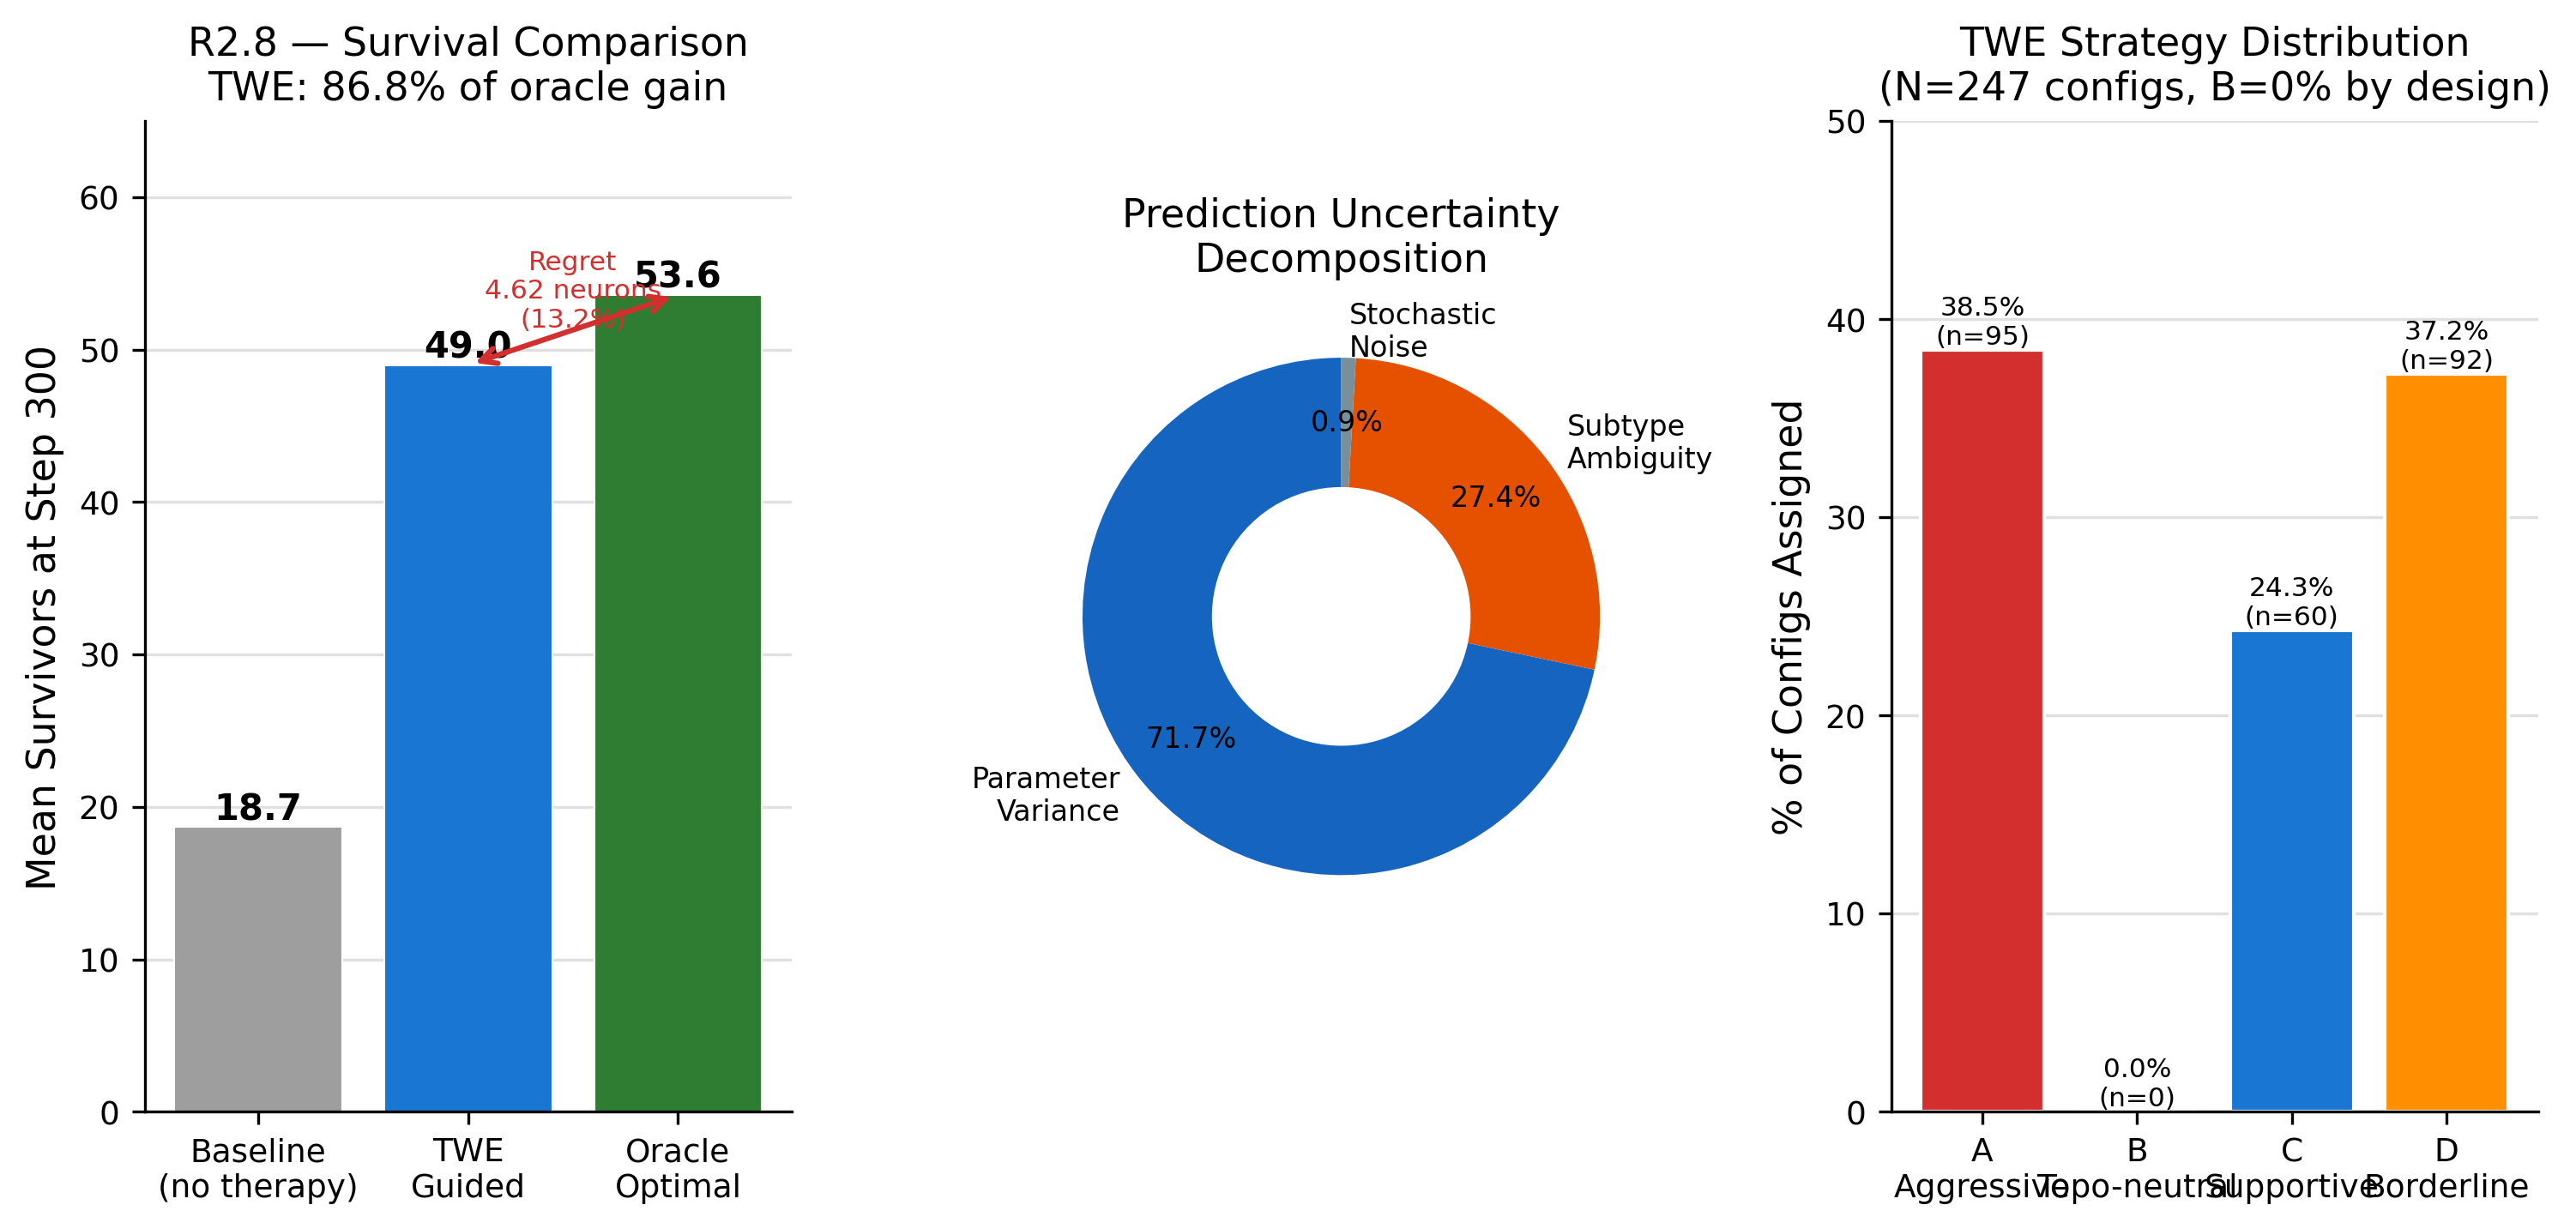
\includegraphics[width=0.9\textwidth]{figures/fig16_r2_twe.png}
\caption{Therapeutic Window Estimator (TWE) performance: survival comparison (TWE-guided
vs.\ oracle-optimal vs.\ baseline), uncertainty decomposition (within-subtype variance 71.7\%,
subtype misclassification 27.4\%, stochastic noise 0.9\%), and strategy distribution across
247 configurations.}
\label{fig:twe}
\end{figure}

%% ============================================================
\clearpage
\section{Discussion}
%% ============================================================

\subsection{A two-tier mechanistic picture}

The central mechanistic conclusion across ten phases of simulation is a two-tier disease model:
an aggregation-driven biochemical cascade (Tier~1) that is sensitive to early intervention, and
a topological load-redistribution cascade (Tier~2) that becomes self-sustaining once enough
neurons have died and is insensitive to biochemical intervention. This distinction has a precise
operational meaning in the model and potentially a conceptual analogue in ALS biology.

In the model, Tier~1 is the rate-limiting step: the irreversible ATP collapse requires
simultaneous high aggregation burden and low ATP, which --- given the log-uniform distribution
of aggregation parameters --- takes approximately 200 simulation steps of silent accumulation
before the threshold is crossed. Tier~2 activates within 20 steps of the first death and
amplifies any loss through load redistribution at a rate that exceeds single-neuron clearance
capacity. The practical consequence is that early therapy (blocking Tier~1) delays Tier~2 by
265 steps, while late therapy (after Tier~2 has activated) cannot reverse the cascade.

Whether ALS biology features an analogous distinction --- between early aggregation-seeding
dynamics that can be targeted by antisense oligonucleotides, and later network-level
compensatory failure that cannot --- is an open question that existing clinical data cannot yet
answer. The model predicts this distinction would manifest as a qualitative difference in
treatment response curves depending on when therapy begins relative to a measurable early
biomarker.

\subsection{Is \texttt{aggregationAmplification} dominance a model artifact or a genuine
system property?}

A sceptical reviewer will note that \texttt{aggregationAmplification} governs regime membership,
subtype identity, therapeutic boundary shape, and cascade velocity --- raising the question of
whether this reflects a genuine dynamical property or merely a consequence of model
parameterisation.

Three lines of evidence argue against pure artifactuality:

\textbf{First}, ablation testing (Phase~7A) demonstrated that setting
\texttt{aggregationAmplification} to zero eliminates genuine tipping points entirely (tipping
step: 221 $\to$ 500, plateau: 10 $\to$ 60 neurons), while disabling all other mechanisms
individually --- ATP collapse, glutamate excitotoxicity, astrocyte support, irreversibility ---
produces negligible regime change.

\textbf{Second}, the clean non-overlapping regime boundaries (stable \texttt{aggAmp} $< 0.30$,
critical 0.30--12.91, runaway $> 12.91$) with a 160-fold separation between stable and runaway
means are consistent with a genuine bifurcation parameter rather than a smoothly varying
influence.

\textbf{Third}, the biological mapping is coherent: \texttt{aggregationAmplification} controls
both intrinsic seeding rate and prion-like spreading efficiency --- exactly the role attributed
to TDP-43 and SOD1 propagation efficiency in ALS pathology literature
\citep{nonaka2013,smethurst2016}. A single parameter that controls both seeding and spreading
will naturally dominate any model that includes both processes.

The honest caveat is that we cannot exclude the possibility that a richer model with additional
coupled feedback pathways (glial reactivity, vascular compromise, immune infiltration) would
distribute control across multiple parameters. Whether pTDP-43 propagation efficiency, as
measured by serial CSF pSer409/410 slope in pre-symptomatic carriers, behaves as a dominant
stratifier of disease course is a directly testable experimental prediction of this model.

\subsection{The pre-symptomatic therapeutic window as a fundamental constraint}

The linear therapeutic boundary ($\mathrm{max\_start\_t} = 425 \times \text{strength} - 237$ for
config~\#334; mean $252 \times \text{strength} - 107$ across 17 configurations) has a direct
interpretation: below a minimum effective strength (${\sim}60\%$ suppression) no prevention is
possible regardless of timing; above this minimum, additional strength linearly extends the
available window but cannot make it unlimited.

The mean conservative boundary ($\mathrm{max\_start\_t} = 132 \times \text{strength} - 224$)
implies that even 80\% suppression may not allow prevention in the most aggressive disease
configurations if therapy begins after symptom onset. This is structurally consistent with the
ATLAS vs.\ VALOR comparison: ATLAS (pre-symptomatic) showed disease delay \citep{benatar2023};
VALOR (post-symptomatic) showed more modest benefits \citep{miller2022}.

We stress several critical limitations of this comparison. First, the model uses no human
biology. Second, the time calibration (1 step $\approx$ 2.25 days) is based on an assumed
pre-symptomatic window of 15 months. Third, the boundary shape may depend on disease parameters
not measured clinically. The qualitative story --- that the window closes before symptom onset
in aggressive cases --- is a hypothesis suggested by the model, not a clinical prediction.

\subsection{Topology and the \textit{C.~elegans} connectome}

The finding that the \textit{C.~elegans} wiring produces 100\% genuine tipping rates while
the Barab\'{a}si-Albert scale-free network produces 0\% is interpretable in terms of network
resilience theory. Scale-free networks resist targeted attacks on hub nodes and distribute
damage broadly \citep{albert2000}. The biological \textit{C.~elegans} motor circuit instead
concentrates vulnerability: its motor neurons are not hubs but are the highest-vulnerability
nodes, and the circuit channels aggregation spread through exactly these nodes.

For the human motor system, the relevant insight is speculative: if the corticospinal-motor
neuron circuit has a structural organisation that concentrates rather than distributes cellular
stress, it would be similarly susceptible to cascade collapse. These are hypotheses only.

\subsection{Disease subtypes and patient stratification}

The $K = 2$ split of all 247 genuine configurations into slow-tipping (\texttt{aggAmp}
$\approx 1.4$, tipping step~224) and fast-tipping (\texttt{aggAmp} $\approx 5.9$, tipping
step~107) disease classes is a model prediction about qualitative disease heterogeneity. If this
model structure has any analogue in ALS biology, it would suggest that the clinically observed
heterogeneity in progression rate may reflect distinct molecular subtypes characterised by
aggregation seeding efficiency, not merely variations in a single continuous variable.

Round~2 (Section~3.12.3) further revealed that these two subtypes respond asymmetrically to
circuit topology modifications, with C1 fast-tipping disease disproportionately harmed by
recurrent feedback loops (triangle-rich interaction~$= +2.16$ favouring C0). If
subtype-specific topology sensitivity has any clinical analogue, this interaction effect
warrants experimental investigation.

\subsection{Robustness hierarchy and the nature of model predictions}

The Phase~14 stress tests reveal that the model's dynamical properties do not all break at the
same perturbation level. Spatial coherence and strict tipping-point classification collapse
relatively early (30\% edge dropout, vulnerability $\sigma = 0.50$), indicating that these
properties depend on fine-grained structural and parametric detail. By contrast, the relative
ordering of degeneration aggressiveness across disease configurations never breaks within the
tested range.

These results motivate a reframing of what the simulator robustly predicts. Although spatial
coherence and strict tipping-point structure collapse under severe perturbation, the relative
ordering of degeneration aggressiveness remains highly preserved, suggesting that disease
severity behaved as a global dynamical invariant (within the tested perturbation range) rather
than a local topological artifact.

\subsection{Round~2: Topology as a disease modifier and the path to clinical translation}

Round~2 demonstrated that sparse connectivity architecture intrinsically resists ALS-like
cascade propagation, while recurrent feedback loops exhibit a critical safety threshold at
${\sim}60\%$ density beyond which cascade vulnerability increases sharply. The finding that no
topology modification widened the therapeutic window --- despite some variants markedly altering
cascade resilience --- is a mechanistically important dissociation: circuit architecture affects
how a cascade propagates but not when pharmacological intervention must begin to prevent it.

The pre-symptomatic biomarker analysis (R2.5b, R2.7, R2.8) represents the most directly
translational finding in the project. The demonstration that three simulation-derived proxies --- conceptually analogous to NfL
trajectory, pTDP-43 phosphorylation rate, and EMG velocity decline --- at a pre-symptomatic
timepoint can classify model disease subtype at 87\% accuracy and guide simulated intervention
strategy to 86.8\% of oracle efficiency suggests a possible simulation-derived framework that,
if validated in biological systems, could inform hypotheses about pre-symptomatic surveillance
in familial ALS contexts. The TWE framework is not a clinical decision tool --- it is a
hypothesis about what such a tool could achieve if the biological analogues of model parameters
were measurable with sufficient precision, and if the model itself were validated against
biological data.

\subsection{Limitations}

\textbf{The model is not biologically calibrated.}
Parameter ranges are chosen for dynamical coverage, not to match measured quantities in any
biological system. Results cannot be mapped to clinical timescales, drug concentrations, or
patient outcomes without independent biological validation.

\textbf{\textit{C.~elegans} is not the human motor system.}
The 61-neuron motor circuit differs from the corticospinal-motor neuron system in scale (orders
of magnitude larger in scale), cell type, connectivity pattern, and evolutionary context.
\textit{C.~elegans} does not develop ALS.

\textbf{The model converges toward a single-factor system in the tested parameter regime.}
Phase~7A ablation demonstrated that the proposed multi-factor cascade (aggregation $\to$ ATP
$\to$ glutamate $\to$ calcium $\to$ ROS) behaves effectively as a single-factor aggregation
model in the explored configurations: disabling every pathway except aggregation produced
negligible change, while disabling aggregation alone eliminated all tipping-point structure.
This is an important mathematical limitation: the cascade architecture is present by design, but
in the tested parameter space, only one factor is load-bearing. All findings should be
interpreted in this context.

\textbf{Aggregation dynamics are highly simplified.}
The model treats aggregation as a scalar quantity with prion-like spread, ignoring spatial
structure of protein aggregation within and between cells, different aggregate species (oligomers
vs.\ fibrils), clearance machinery (proteasome, autophagy), and heterogeneous molecular
mechanisms of different ALS subtypes (SOD1, TDP-43, FUS, C9ORF72).

\textbf{Parameter exploration is incomplete.}
500 configurations cannot cover a 7-dimensional parameter space thoroughly. Parameter
interactions beyond the identified cascade structure are not characterised.

\textbf{The therapeutic comparison is not directly translatable.}
The therapy-class comparison (Phase~6) tests abstract parameter modifications, not real drugs.

\textbf{Early-warning signals are computational proxies, not validated biomarkers.}
The three features used in Round~2 (\texttt{atp\_decline\_50}, \texttt{stress\_velocity\_50},
\texttt{agg\_slope\_50}) are abstract dynamical quantities within the simulator. Their mapping
to clinical measurements (NfL, pTDP-43, EMG) is a conceptual analogy, not a calibrated
correspondence. No clinical data was used to derive or validate these mappings. The term
``biomarker'' is avoided in this paper precisely for this reason.

\textbf{Round~2 calibration is unvalidated.}
Every clinical timeline in Round~2 depends on the single-anchor assumption that 1~step
$\approx$ 2.25~days. This has not been validated against clinical data in any ALS cohort.

\textbf{$N = 247$ configurations is modest for unsupervised clustering.}
K-means results should be treated as directional hypotheses, not established disease categories.
Silhouette scores (0.41--0.43) indicate soft cluster boundaries.

\textbf{The multi-factor cascade is functionally dominated by aggregation in tested regimes.}
Other pathways may become relevant at different parameter values or with stronger inter-pathway
coupling. This is a priority for future investigation.

\textbf{\texttt{aggregationAmplification} as a single compound parameter is a design limitation.}
This parameter controls both intrinsic seeding rate and synaptic spreading efficiency within a
single multiplicative term. Its dominance may therefore reflect the coupling design rather than
a discovered biological property.

\textbf{Priority for future development.}
The most important next step is to decouple \texttt{aggregationAmplification} into two
independent parameters: (1) intrinsic intracellular seeding rate and (2) trans-synaptic
spreading efficiency. This would test whether dominance is an artifact of coupling, or whether
one sub-process is genuinely rate-limiting. Until this is done, single-parameter dominance
should be treated as a model property, not a biological claim.

%% ============================================================
\clearpage
\section{Conclusion}
%% ============================================================

We present a systematic multi-phase computational study of degeneration dynamics on the
\textit{C.~elegans} motor connectome, extended through Round~2 to topology resilience and
proof-of-concept early-warning signal analysis. Our principal findings, subject to the
limitations stated above, are:

\begin{enumerate}
\item \textbf{Criticality is an emergent property whose local manifestations (spatial coherence,
tipping-point timing) are moderately fragile, but whose global expression (relative degeneration
aggressiveness) constitutes a dynamical invariant (within the explored perturbation range) robust to severe structural perturbation.}
64.7\% of explored parameter space shows genuine triphasic degeneration (falsified against a
null model at 0\% FPR using a spatial-coherence criterion).

\item \textbf{Aggregation amplitude is the dominant bifurcation parameter}, spanning 160-fold
across regimes and predicting 84.6\% of disease subtype membership from a single threshold.

\item \textbf{Aggregation suppression is the most effective therapeutic strategy} across all
tested mechanisms, because all downstream biochemical pathways (ATP, glutamate, calcium) are
aggregation-gated and cannot sustain degeneration independently.

\item \textbf{A topological load-redistribution escape pathway exists} that is
aggregation-independent and capable of complete collapse in isolation, establishing a two-tier
disease model with distinct therapeutic targets.

\item \textbf{A sharp linear therapeutic boundary} governs prevention: below a minimum
effective strength or beyond a maximum tolerated delay, no intervention prevents collapse. The
boundary generalises across 17 of 20 tested configurations ($R^2 = 0.83$) with substantial
inter-configuration heterogeneity (slope standard deviation 120), is unchanged by topology
modifications, and is predictable from $t=50$ biomarkers at $r=0.765$.

\item \textbf{Two fundamental disease subtypes} are identified by unsupervised clustering on
simulation-only features: slow-tipping (\texttt{aggAmp} $\approx 1.4$, tipping step
$\approx 224$) and fast-tipping (\texttt{aggAmp} $\approx 5.9$, tipping step $\approx 107$),
with qualitatively different predicted therapeutic windows and asymmetric sensitivity to
connectome modifications.

\item \textbf{Sparse-chain topology intrinsically resists ALS-like cascade propagation}
(RES~$=0.815$ vs.\ baseline 0.800), while triangle-rich feedback loops above 60\% density are
actively destabilising (RES~$=0.738$, plateau survivors $-30\%$ relative to baseline). No
topology modification tested in Round~2 widened the pre-symptomatic therapeutic window,
confirming that circuit architecture and pharmacological timing are independent intervention axes.

\item \textbf{Pre-symptomatic subtype classification from three early biomarkers is feasible in
simulation}: 88.3\% accuracy at $t=50$ (before any neuron death in slow-tipping configurations)
from simulation-derived proxies conceptually analogous to NfL trajectory, pTDP-43
phosphorylation rate, and EMG velocity decline (unvalidated conceptual mappings), with the
logistic regression calibrated across all five confidence bins.

\item \textbf{A pre-symptomatic Therapeutic Window Estimator achieves 86.8\% of the oracle-defined
benefit within this simulation framework} (regret: 4.62 neurons, 13.2\% of achievable gain) across 247 genuine disease
configurations. Within-subtype parameter heterogeneity (71.7\% of prediction variance) --- not
stochastic noise (0.9\%) --- is the dominant irreducible error source, directly motivating
clinical measurement of \texttt{aggAmp} analogues as the highest-yield experimental priority.
\end{enumerate}

Findings were robust to $\pm 20\%$ synaptic weight noise, $\pm 20\%$ vulnerability score
perturbation, 10\% edge dropout, and $\pm 20\%$ per-neuron aggregation heterogeneity.
Stress-testing to extreme levels reveals a robustness hierarchy: spatial coherence and strict
tipping-point structure break at 30\% edge dropout and vulnerability $\sigma = 0.50$, while
the relative ordering of degeneration aggressiveness across disease configurations is never
disrupted, persisting as a dynamical invariant within the tested perturbation space even when 70\% of synaptic connections are
removed.

These findings are hypothesis-generating. They motivate specific experimental questions: Does
early biomarker detection and intervention provide qualitatively better outcomes than post-onset
treatment in SOD1-ALS carriers? Do different ALS molecular subtypes have measurably different
rates of network-level compensatory failure? Is there evidence for a load-redistribution cascade
in the pattern of motor neuron loss during ALS progression? Are pTDP-43 accumulation rates
bimodally distributed in pre-symptomatic familial ALS cohorts, consistent with two
aggregation-amplification subtypes?

We hope this modelling framework --- and particularly the falsification methodology, two-tier
mechanistic model, therapeutic boundary quantification, dynamical robustness hierarchy, and
pre-symptomatic Therapeutic Window Estimator --- may contribute to the conceptual toolkit used
to reason about ALS disease dynamics and intervention timing, while remaining clear that
experimental validation at every level is required before any translational implications can
be considered.

%% ============================================================
\clearpage
\section*{Data Availability}
\addcontentsline{toc}{section}{Data Availability}
%% ============================================================

The complete simulation engine, phase-by-phase results (JSON), and figures are available at:
\url{https://github.com/MaryamRezaeeNl/als-connectome}

An interactive web-based visualization of all phases and findings is available at:
\url{https://als-connectome-dashboard.vercel.app}

Key output files:
\begin{itemize}
\item \texttt{results/regime\_map.json} --- 500-configuration parameter sweep and regime classifications
\item \texttt{results/phase7b\_strict\_criterion.json} --- strict tipping criterion results for all 382 critical configurations
\item \texttt{results/phase9\_phase\_diagram.json} --- full 99-point therapeutic boundary grid
\item \texttt{results/phase10\_boundary\_robustness.json} --- boundary robustness across 20 configurations
\item \texttt{results/phase12\_validation.json} --- subtype clustering on 247 configurations
\item \texttt{results/phase14\_breaking.json} --- breaking threshold probe (extreme dropout and vulnerability noise)
\item \texttt{results/r2\_therapeutic\_window\_estimator.json} --- TWE full results: OOF predictions, triage simulation, uncertainty decomposition
\end{itemize}

\bibliographystyle{plainnat}
\bibliography{references}

\end{document}
